\documentclass[12pt]{article}
\usepackage{amsmath,amsfonts,nicefrac}
\usepackage{graphicx}
\usepackage{enumerate}
\usepackage{natbib}
\usepackage{url} % not crucial - just used below for the URL 
\usepackage{ifthen}
\usepackage{subcaption}

%\pdfminorversion=4
% NOTE: To produce blinded version, replace "0" with "1" below.
\newcommand{\blind}{1}
% DON'T change margins - should be 1 inch all around.
%\addtolength{\oddsidemargin}{-.5in}%
%\addtolength{\evensidemargin}{-.5in}%
%\addtolength{\textwidth}{1in}%
%\addtolength{\textheight}{-.3in}%
%\addtolength{\topmargin}{-.8in}%

\usepackage[margin=0.5in]{geometry}
\usepackage[table]{xcolor}% http://ctan.org/pkg/xcolor

\newcommand{\cl}[2]{\cellcolor{#1!#2}}
\newcommand{\inc}[2]{ \ifthenelse{\equal{#1}{1}}{\input{./sections/#2}}{ } }



\begin{document}

\def\spacingset#1{\renewcommand{\baselinestretch}%
{#1}\small\normalsize} \spacingset{1}


%%%%%%%%%%%%%%%%%%%%%%%%%%%%%%%%%%%%%%%%%%%%%%%%%%%%%%%%%%%%%%%%%%%%%%%%%%%%%%

\if1\blind
{
  \title{\bf A Structured Framework for Bayesian \\Sequential Monitoring in Clinical Trials}
  \author{Evan Kwiatkowski\textsuperscript{$\dagger$}, 
	        Eugenio Andraca-Carrera\textsuperscript{$\ddagger$},\\
					Mat Soukup\textsuperscript{$\ddagger$},
					\medskip Matthew A. Psioda\textsuperscript{$\dagger$}\thanks{The authors gratefully acknowledge \textit{please remember to list all relevant funding sources in the unblinded version}}\\
	  %
	  $\dagger$ Department of Biostatistics,
		University of North Carolina, \\
		McGavran-Greenberg Hall, CB\#7420, \\
		%
		\medskip Chapel Hill, North Carolina, U.S.A.\\
    $\ddagger$ Division of Biometrics VII, Office of Biostatistics \\
		           Center for Drug Evaluation and Research, \\
							 US Food and Drug Administration, \\
							 Silver Spring, Maryland, USA \\									
		}
  \maketitle
} \fi

\if0\blind
{
  \bigskip
  \bigskip
  \bigskip
  \begin{center}
    {\LARGE\bf Title}
\end{center}
  \medskip
} \fi

\bigskip
\begin{abstract}
Conclusions from Bayesian sequential monitoring are coherent when specification of prior distributions are intuitively related to the research objectives. A compelling level of evidence is required to terminate enrollment for either efficacy or futility. This paper defines monitoring priors using generalized normal distributions parameterized via three specified quantities (mode and two tail probabilities), which reflect prior belief defined using a consistent definition of compelling level of evidence. These concepts are demonstrated through simulations based on a single-arm proof-of-activity trial in pediatric ulcerative colitis and a parallel two-group design in pediatric lupis.
\end{abstract}

\noindent%
{\it Keywords:}  Generalized normal distribution, monitoring priors, real world evidence
\vfill

\newpage
\spacingset{1.5} % DON'T change the spacing!

\section{Introduction}

A goal of the 21st Century Cures Act \citep{USCongress2016} is to expedite the approval process for new drugs and devices through the incorporation of real-world evidence into clinical trial data summaries. Similarly, an objective of the Prescription Drug User Fee Act VI  is to enhance the capacity to review ``complex adaptive, Bayesian, and other novel clinical trial designs." \citep{FDA2017} Bayesian designs are natural for incorportating external evidence through prior distributions. This is useful in areas where clinical trials would take a lot of time due to slow enrollment or long follow-up periods, and where relevant external data exists. For example, a treatment for a rare pediatric disease might have difficulties with enrollment, and there may be relevant data from adult trials which could augument the trial findings and lead to a conclusion of efficacy sooner. Group sequential designs also have the possible benefits of leading to conclusions earlier, saving time and resources, as well as reducing the exposure of patients to inferior treatments. Bayesian sequential designs which incorporate external evidence therefore have a much increased capacity to expedite the approval process for effective treatments, but they most be carefully planned. The effects of interim analyses and the informativeness of the priors must be well understood. This paper presents a structured or default way to determine prior distributions based on the trial design. Our major contribution is to present methods for the default or automatic selection of prior distributions in a way that is applicable to a wide array of clinical trial designs.

The likelihood principle asserts that any data with the same likelihood function should lead to the same conclusion \citep{Berger1988}. In the context of sequential analysis of clinical trials, the stopping rule that led to the termination of data collection is irrelevant to the conclusion \citep{Barnard1947,Anscombe1963,Cornfield1966a,Cornfield1966b}. It is most succinctly as ``It is entirely appropriate to collect data until a point has been proven or disproven, or until the data collector runs out of time, money, or patience."\citep{Edwards1963}. Bayesian conclusions are not affected by frequent or even continual monitoring of the data, and such interim analyses should be encouraged to terminate data collection if appropriate \citep{Berry1989,Berry1993,Spiegelhalter1994}.

Interpretation of conclusions from the Bayesian perspective is natural when specification of prior distributions are intuitively related to the research objectives (e.g. skeptical and enthusiastic priors)  \citep{Freedman1989,Freedman1992,Spiegelhalter1993,Fayers1997} which is necessary for regulatory agencies \citep{Parmar1993}. Bayesian monitoring is further formalized by specifying the loss function via decision theory \citep{Carlin1998}.

The most common Bayesian metrics for assessing evidence at interim analyses are posterior probabilities and predictive probabilities, and the choice of metric depends on research objective. Posterior probabilities assess the level of evidence in favor of the null or alternative hypothesis, and predictive probabilities determine the capacity for the trial to show convincing evidence in favor of the alternative hypothesis if more outcomes are ascertained. This paper uses posterior probabilities to highlight how the level of evidence at interim analyses is linked to monitoring prior specification.

Frequentist group sequential designs use spending functions associated with Type I and Type II error \citep{Pocock1977,OBrien1979}. While it is possible to calibrate a Bayesian design to have exact pre-specified frequentist properties \citep{Kopp-Schneider2019}, this re-introduces inflexibility (e.g. interim analyses must be pre-specified) that is unnecessary using a fully Bayesian method. Therefore, the objective is to present operating characteristics generally that are ``well-calibrated" \citep{Grieve2016} but not motivated by strict adherence to pre-specified thresholds.

This paper is organized as follows: Section \ref{sec:methods} contains a brief review of Bayesian hypothesis testing using posterior probabilities, and describes the method for defining monitoring and inference priors. Examples are in Section \ref{sec:examples}, with Section \ref{sec:example1} containing a one-arm study and Section \ref{sec:example2} a two-arm study.

\section{Methods}\label{sec:methods}
%\subsection{Monitoring versus Estimation Priors}
%\begin{itemize}
% \item Define generally in terms of $\boldsymbol\theta = \left( \gamma, \boldsymbol\psi  \right)$ where $\gamma$ is a parameter of interest
%       and $\boldsymbol\psi$ is a nuisance parameter (possible vector valued).
% \item Define \textit{Monitoring} Priors and \textit{Inference} Priors.
% \item Make connection between Inference priors and two-part mixture prior and BMA.
% \item Define \textit{Skeptical} and \textit{Enthusiastic} monitoring priors and how each would be used.
% \item I would have a generic graphic to illustrate the types of priors and the mixture.
% %\item Motivate in the context of a simple example (i.e., single parameter binary example).
%\end{itemize}

\subsection{Preliminaries}\label{sec:preliminaries}
\subsubsection{Bayesian Hypothesis Testing}
Consider a clinical trial application where the primary objective is to test a hypothesis about an unknown quantity of interest which we denote by $\theta$ with possible values
for $\theta$ falling in the parameter space $\Theta$.
%
For example, in a single-arm trial with binary response endpoint, $\theta \in (0,1)$ may be the response probability associated with patients receiving the investigational treatment.
%
For a two-arm trial with binary response primary endpoint, $\theta \in (-1,1)$ may be the difference in response probabilities between patients receiving the investigational treatment 
and those receiving the control treatment (e.g., placebo).

Throughout the paper we will let $\mathbf{D}$ represent the data collected in a trial at some point in time. 
%
For example, for the two-arm trial example above and assuming no covariates other than the treatment indicator, $\mathbf{D}=\left\{y_i,z_i:i=1,...,n\right\}$ where $y_i$ is an 
indicator of response for patient $i$ and $z_i$ is an indicator for whether patient $i$ was assigned the investigational treatment.
%
We use the generic representation $p(\mathbf{D}|\theta,\psi)$ to reflect the density or mass function for the collective data $\mathbf{D}$ as a function of $\theta$ and potential nuisance parameters
$\psi$ which could be multidimensional.
%
For example, for the two-arm trial example above $\psi$ would correspond to the response probability for patients receiving the control treatment.


Consider the hypotheses $H_0:\theta\in\Theta_{0}$ versus $H_1:\theta\in\Theta_{1}$ where $\Theta_{0}\bigcup \Theta_{1} = \Theta$ and $\Theta_{0} \bigcap \Theta_{1} = \emptyset$.
%
Formal Bayesian hypothesis testing requires the specification of prior probabilities on the hypotheses (e.g., $p(H_i)$ for $i=0,1$)
and prior distributions for $\left(\theta,\psi\right)$ specified over the parameter space defined with respect to each of the 
hypotheses (e.g. $\pi\left(\theta,\psi \big| H_i\right)$ for $i=0,1$). 
%
For ease of exposition, for the remainder of Section~\ref{sec:preliminaries}, we will focus on the case where $\theta$ is the 
only unknown parameter and ignore $\psi$.

The posterior probability of hypothesis $H_i$ is given by 
\begin{eqnarray*}
p(H_i|\mathbf{D})&=\frac{p(\mathbf{D}|H_i)\cdot p(H_i)}{p(\mathbf{D}|H_0)\cdot p(H_0)+p(\mathbf{D}|H_1)\cdot p(H_1)},
\end{eqnarray*}
where $p(\mathbf{D}|H_i) = \int_{\Theta_i} p(\mathbf{D}|\theta)\pi(\theta|H_i)d\theta$ is the marginal likelihood associated with hypothesis $H_i$.
%
In practice, most Bayesian methods for clinical trials perform hypothesis testing based on the posterior probability of the \textit{event defining $H_i$}.
%
For this approach, one simply needs to specify a prior $\pi\left(\theta\right)$ representing belief about $\theta$ overall and compute the posterior distribution.
%
The posterior probability that $\theta\in\Theta_i$ is given by
\begin{equation}
P(\theta\in\Theta_i|\mathbf{D})
=\frac{\int_{\Theta_i} p(\mathbf{D}|\theta)\pi (\theta)d\theta}{\int_{\Theta}p(\mathbf{D}|\theta)\pi(\theta) d\theta}
=\frac{\int_{\Theta_i} p(\mathbf{D}|\theta)\pi (\theta|\theta\in\Theta_i)d\theta\cdot P(\theta\in\Theta_i)}
      { \sum_{j=0,1} \int_{\Theta_j}p(\mathbf{D}|\theta)\pi (\theta|\theta\in\Theta_j)d\theta\cdot P(\theta\in\Theta_j) } \label{eq:equation1},
\end{equation}
where $P(\theta\in\Theta_i)=\int_{\Theta_i}\pi(\theta)d\theta$. 
%
From \eqref{eq:equation1} we can readily see that the $P(\theta\in\Theta_i|\mathbf{D})$ is equal to $p(H_i|\mathbf{D})$ if one takes
$p(H_i) =P(\theta\in\Theta_i)$ and $\pi\left(\theta \big| H_i\right) = \pi\left(\theta\big|\theta \in \Theta_i\right)$ for $i=0,1$.
%
If in fact $\pi\left(\theta\right)$ does represent belief about $\theta$, these choices are perhaps the most intuitive and thus 
we should have no reservation referring to $P(\theta\in\Theta_i|\mathbf{D})$ as the probability that hypothesis $H_i$ is true.
%
For these reasons, in what follows we will refer to the quantity $P(\theta\in\Theta_1|\mathbf{D})$ 
as the posterior probability of $H_i$ for ease of exposition.

\subsubsection{Formalizing the Concept of Substantial Evidence}
For testing one-sided hypotheses such as $H_0: \theta \le 0$ versus $H_0: \theta > 0$ using posterior probabilities, the null hypothesis 
is rejected when $P(\theta > 0 |\mathbf{D})>0.975$.
%
Leveraging this common practice, we define the posterior probability threshold $1-\epsilon=0.975$ to be the threshold for what constitutes 
\textit{substantial evidence} in favor of a claim (e.g., that $\theta > 0$) and, correspondingly, we refer to $\epsilon$ as the threshold 
for insignificant $\textit{residual uncertainty}$.
%
Our purpose in this paper is not to debate the appropriateness of using $0.975$ as a threshold for defining substantial evidence but rather to 
develop a strategy for prior elicitation that leverages an accepted threshold to make prior elicitation more structured for sequentially monitored 
trials in hopes that this added structure facilitates the use of sequential monitoring more broadly.

Formally, we say that an individual whose belief is summarized by the distribution $\pi\left(\theta\right)$ is \textit{all but convinced} that $H_i$ is true if 
\begin{align}\label{eq:compellingevidence}
		P_\pi(\theta\in\Theta_i)= 1-\epsilon,
\end{align} 
where the subscript $\pi$ in \eqref{eq:compellingevidence} is simply to indicate that the probability is calculated based on $\pi\left(\theta\right)$ which could be either a prior
or posterior distribution.

\subsubsection{Skeptical and Enthusiastic Monitoring Priors}\label{sec:MP}
Having formalized concepts for \textit{substantial evidence} and  being \textit{all but convinced} of a claim, 
we can now develop a structured framework for constructing skeptical and enthusiastic monitoring priors which will be used to 
determine early stopping rules for efficacy and futility, respectively.
%
The use of monitoring based on changing the opinion of skeptical and enthusiastic observers has been described as overcoming a 
handicap \citep{Freedman1989} and providing a brake \citep{Fayers1997} on the premature termination of trials, and as 
constructing ``an adversary who will need to be disillusioned by the data to stop further experimentation" \citep{Spiegelhalter1994}. 
%
Skeptical and enthusiastic monitoring priors represent to extreme but plausible beliefs about the quantity of interest $\theta$ relative to the hypotheses to be tested.
%
The purpose of monitoring priors to is help answer the question ``Is the evidence compelling enough to stop enrollment for the trial or possibly end it altogether?''
%
Monitoring priors are during for interim analyses of the data. 
%from subjects who completed follow-up while additional outcomes are pending. 
A promising interim analysis that provides substantial evidence of efficacy may justify ending enrollment, while presumably enrolled subjects would continue 
to receive the treatment for the pre-planned period of exposure. 
%
A discouraging interim analysis that provides substantial evidence of futility may justify ending enrollment, and may call for enrolled patients 
who are ongoing in the trial to be transitioned off the investigational treatment (i.e., termination of investigation of the treatment). 
%
For the Bayesian, the question becomes ``From what prior perspective must the evidence be substantial to justify one of the two actions described above?''.
%
A key contribution of this work is to give rationale definitions for an a priori skeptical and enthusiastic perspectives that can be used for early stopping decisions 
in favor of efficacy and futility, respectively.


For ease of exposition, consider the hypotheses $H_0: \theta \le 0$ versus $H_0: \theta > 0$ where $\theta$ represents a treatment effect of interest and let $\theta_1>\theta_0$ 
represent a plausible, clinically meaningful effect.
%
We define an enthusiastic prior $\pi_{E}(\theta)$ as a prior that suggests $\theta_1$ is the most likely value of $\theta$ 
and that reflects the belief of an observer who is \textit{all but convinced} that $H_1$ is true a priori. 
%
Formally, this is defined as the prior satisfying
\begin{align}\label{eq:skptprior}
P_E(\theta >\theta_0)=1-\epsilon,
\end{align}
where the subscript $E$ indicates that the probability is based on $\pi_{E}(\theta)$.
%
Similarly, we define a skeptical prior $\pi_{S}(\theta)$ as a prior that suggests $\theta_0$ is the most likely value of $\theta$ 
and that reflects the belief of an observer who is \textit{all but convinced} that $\theta <\theta_1$ is true a priori. 
%
Formally, this is defined as the prior satisfying
\begin{align}\label{eq:enthprior}
P_S(\theta <\theta_1| \pi_{S})=1-\epsilon.
\end{align}
%
In what follows we refer to \eqref{eq:skptprior} and \eqref{eq:enthprior} as \textit{tail-probability constraints}.

Note that the development of the skeptical prior does not generally reflect skepticism that the alternative hypothesis is true. 
%
Indeed, in most cases the \textit{induced} prior model probabilities based on \eqref{eq:equation1} will be such that $p(H_0) \approx p(H_1)$.
%
This prior simply reflects that $\theta \ge \theta_1$ is exceedingly unlikely and is therefore 
consistent with their being clinical equipoise about the two hypotheses.
%

Unlike the frequentist approach, the degree to which evidence in favor of a hypothesis is substantial is influenced by 
the prior distribution on the quantity of interest.
%
It is natural that one would stop a trial early in favor of efficacy or futility when the evidence in favor of that claim is compelling
to an a priori skeptic or enthusiastic observer, respectively, as defined above.
%
For example, if at any point data sufficiently convince an observer whose prior belief is in accordance with $\pi_{S}(\theta)$ that in fact
the alternative is true, then most any rational observer would also be convinced and therefore ceasing the collection of data
to prove that claim would be reasonable.
%
Similarly, if at any point data sufficiently convince an observer whose prior belief is in accordance with $\pi_{E}(\theta)$ that in fact
the effect of interest is less than what was originally believed, then most any rational observer would also be convinced and therefore ceasing 
the collection of data altogether would be reasonable.

\subsubsection{Maximum Sample Size and Formal Stoppage Criteria}
In this section we formalize a stopping criteria for futility and efficacy and give general 
advice for specifying a maximum sample size for the trial.
%
Through sequentially monitored trials in principle require no fixed sample size, in practice due to resource 
constraints it will almost always be the case that a maximum sample size exists. 
%
Resources permitting, the maximum sample size, denoted by $N$, should be chosen so that there is a 
high probability that the trial generates substantial evidence from the perspective of the skeptic when in 
fact $\theta \approx \theta_1$ in a scenario where the data are only examined once when the full set of 
outcomes are ascertained.
%
The rationale behind this strategy is that one would want to ensure the trial's sample size is sufficient so that
there is high probability the data collected will provide compelling evidence of treatment benefit to observers 
having relatively extreme skepticism regarding the magnitude of treatment benefit a priori.  


For a sequentially monitored trial, observed data are analyzed as often as is feasible in accordance with 
the cost and/or logistical challenges of assembling the necessary data.
%
For example, if an outcome requires adjudication by a committee of clinical experts, it may not be possible to analyze the
data after each patient's outcome data are available due to scheduling or other constraints on the adjudication panel.
%
In other scenarios, a patient's outcome may be based on a laboratory parameter's change after a fixed period of time
and the rate limiting factor for sequential monitoring will be how quickly samples can be shipped, processed, and entered
into a database for analysis.  
%
The strategies presented herein for sequential monitoring are appropriate regardless of how frequently data can be monitored
even if the motivation for sequential monitoring is scenarios where frequent monitoring is feasible.


The skeptic becomes convinced that a treatment is effective if at some point, the observed data suggest there is 
substantial evidence that the alternative hypothesis is true. 
%
Formally, this requires $P_E(\theta>\theta_0| \mathbf{D})>1-\epsilon$, where $\mathbf{D}$ is the observed data at 
that point in time.
%
Note that the evidence must exceed the threshold for what defines it being substantial.
%
When the evidence in favor of the alternative surpasses this threshold, it may no longer be necessary to enroll patients
for the purpose of proving treatment efficacy.


For futility monitoring, at first thought it may seem appealing to stop the trial when the enthusiast becomes convinced that the
null hypothesis is true. 
%
However, for this to be the case the observed data must suggest $\theta \ll \theta_0$ since when $\theta=\theta_0$,
$P_E(\theta\le\theta_0| \mathbf{D}) \rightarrow 0.5$ for large samples sizes.
%
For this reason, we consider a different approach.
%
Recalling that $\theta_1$ represents a plausible, clinically meaningful treatment effect, we define $\theta_{m}= c \cdot \theta_0 + (1-c) \cdot \theta_1$ for 
$c \in [0,1]$ to be a less than desirable treatment effect such, that if it is the case that $P_E\left(\theta<\theta_{m}\Big| \mathbf{D}\right)>1-\epsilon$, 
the trial may be stopped due to have a low probability of having a meaningful treatment effect.
%
For example applications in this paper, we consider $c=0.5$.

\subsection{Monitoring Prior Specification}

The enthusiastic and skeptical priors discussed is Section~\ref{sec:MP} are not uniquely specified based on the requirements discussed in that section. 
%
In this section discussed a family of probability distributions using which we develop more complete 
specifications of the priors above.


The distributions defined in \eqref{eq:enthprior}, \eqref{eq:skptprior} each have a required 
center (modal value) and tail-probability constraint, however, there are still many ways to parametrize such distributions. 
%
The specification of the mean and variance of a normal distribution completely specifies the modal value and tail-probability constraints, and is therefore sufficient for defining enthusiastic and skeptical priors.

\subsubsection{Normal Family of Distributions}
The specification of the mean and variance of a normal distribution completely specifies the modal value and a tail-probability constraint, and is therefore sufficient for defining enthusiastic and skeptical priors.

Consider specifying a skeptical prior as a normal distribution $\mathcal{N}(\mu,\sigma)$ with modal value $\theta_0$ satisfying $P(\theta<\theta_1)=1-\epsilon$ with $\theta_0<\theta_1$. The mean and the mode align so $\mu=\theta_0$, and it is left to specify $\sigma$. Let $\Phi$ denote the cumulative distribution function for a standard normal distribution, and $\Phi^{-1}$ denote the quantile function. The standard deviation $\sigma$ is specified as $\sigma=\frac{\theta_1-\theta_0}{\Phi^{-1}(1-\epsilon)}$. It follows that $(\mu,\sigma)$ can always be specified to have a desired modal value and tail-probability constraint, and therefore can be used to specify skeptical and enthusiastic priors.

Recall that $\theta_m$ represented a less than desireable treatment effect between $\theta_0$ and $\theta_1$ (e.g. $\theta_m=\frac{\theta_0+\theta_1}{2}$). Since the normal distribution is completely specified by $(\mu, \sigma)$, quantities such as $P(\theta<\theta_m)$ are also specified. For example, for the skeptical prior defined above with $P(\theta<\theta_1)=1-\epsilon$ it follows that $P(\theta<\frac{\theta_0+\theta_1}{2})=\Phi(\frac{\Phi^{-1}(1-\epsilon)}{2})$. In particular, if $P(\theta<\theta_1)=0.975$, then $P(\theta<\frac{\theta_0+\theta_1}{2})=0.836$, equivalently, $P(\theta\in(\frac{\theta_0+\theta_1}{2},\theta_1))=0.139$. Let $\gamma=P(\theta\in(\frac{\theta_0+\theta_1}{2},\theta_1))$. 
A second tail-probability constraint for a skeptical prior is
\begin{align}\label{eq:skptpriortail}
P(\theta<\frac{\theta_0+\theta_1}{2})=\epsilon+\gamma
\end{align}
for $\gamma>\epsilon$. 
As discussed above, the quantity $\gamma$ is determined by the choice of $(\mu,\sigma)$ in the normal distribution, but it can be specified by a distribution that has three parameters, as shown in the next section. The flexibility to modify $\gamma$ can change the prior to be flatter or more concentrated around the modal value. If $\gamma>\Phi(\frac{\Phi^{-1}(1-\epsilon)}{2})$ then the distribution will be more concentrated around the modal value, and if $\gamma<\Phi(\frac{\Phi^{-1}(1-\epsilon)}{2})$ then the distribution will be flatter around the modal value.

\subsubsection{The Generalized Normal Family of Distributions}
We will consider the generalized normal distribution \citep{Nadarajah2005} for prior specification. The density for a generalized normal distribution $\mathcal{GN}(\mu,\alpha,\beta)$ is
\begin{align}\label{eq:generalizednormalkernel}
f(\theta)=\frac{\beta}{2\alpha\Gamma(1/\beta)}\exp\left\{-\left(\frac{|\theta-\mu|}{\alpha}\right)^\beta\right\}
\end{align} where $\mu\in\mathbb{R}$ is a location parameter, $\alpha>0$ is a scale parameter, and $\beta>0$ is a shape parameter. Note that $\beta=2$ corresponds to the normal distribution. Let $F_{\mu,\alpha,\beta}$ denote the cumulative distribution function of $\mathcal{GN}(\mu,\alpha,\beta)$. An expression for $F_{\mu,\alpha,\beta}$ is provided in the appendix.
%The quantile function for $p\in (0,1)$ is 
%\begin{align}
%Q(p;\mu,\alpha,\beta)=sign(p-0.5) g\left(2|p-0.5|;\frac{1}{\beta}\left(\frac{1}{\alpha}\right)^{\beta}\right)^{1-\beta}+\mu,
%\end{align}
%where $g\left(2|p-0.5|;\frac{1}{\beta}\left(\frac{1}{\alpha}\right)^{\beta}\right)$ refers to the inverse CDF for a gamma distribution with shape $\frac{1}{\beta}$ and rate $(\frac{1}{\alpha})^\beta$ evaluated at $2|p-0.5|$.

Consider creating a skeptical prior that is centered around $\theta_0$ and satisfies the tail-probability conditions of \eqref{eq:skptprior} and \eqref{eq:skptpriortail}. As with the normal distribution, $\mu=\theta_0$. We minimize the function $(F_{\mu,\alpha,\beta}(\theta_1)-(1-\epsilon))^2+(F_{\mu,\alpha,\beta}(\frac{\theta_0+\theta_1}{2})-(1-(\epsilon+\gamma)))^2$ with respect to $(\alpha,\beta)$ to find the scale and shape parameters.

These distributions can be truncated to represent the domain of $\theta$ (e.g. a response probability in (0,1)) as demonstrated in Section \ref{sec:example1model} and \ref{sec:example2model}.

Examples of skeptical and enthusiastic priors are displayed in Figure \ref{fig:figure5}.
%\begin{align}\label{eq:enthprior_tail1}
%Q(\theta_0:\mu=\theta_1,\alpha,\beta)=\epsilon
%\end{align} and that also satisfies a second tail-probability condition 
%\begin{align}
%Q\left(\frac{\theta_0+\theta_1}{2};\mu=\theta_1,\alpha,\beta\right)=\epsilon+\gamma \label{eq:enthprior_tail2}
%\end{align}
%for $\gamma>\epsilon$. There is a unique combination of $\alpha$ and $\beta$ that satisfy \eqref{eq:enthprior_tail1} and \eqref{eq:enthprior_tail2}.
%
%
%The modification of $\beta$ can be used to concentrate or flatten the distribution around the modal value. If $\beta<2$ then the distribution becomes more peaked relative to a normal distribution, and if $\beta>2$ then the distribution becomes flatter. Examples of skeptical and enthusiastic priors for a single parameter $\theta$ based on the trial from Section \ref{sec:preliminaries} are displayed in Figure \ref{fig:figure1}. The location and shape parameters are pre-specified, and the scale parameter is chosen to satisfy the tail-probability constraints \eqref{eq:enthprior}, \eqref{eq:skptprior}.

%Continuing the trial setup from Section \ref{sec:preliminaries}, it is necessary to truncate the generalized normal distribution to the range $[0,1]$. When truncated to the unit interval, this density becomes
%\begin{align}\label{eq:generalized_normal_univariate}
%\pi(\theta)\propto \exp\left\{-\frac{|\theta-\mu|}{\alpha}^\beta\right\} I(\theta\in[0,1]).
%\end{align} 
%

\begin{figure}\begin{center}
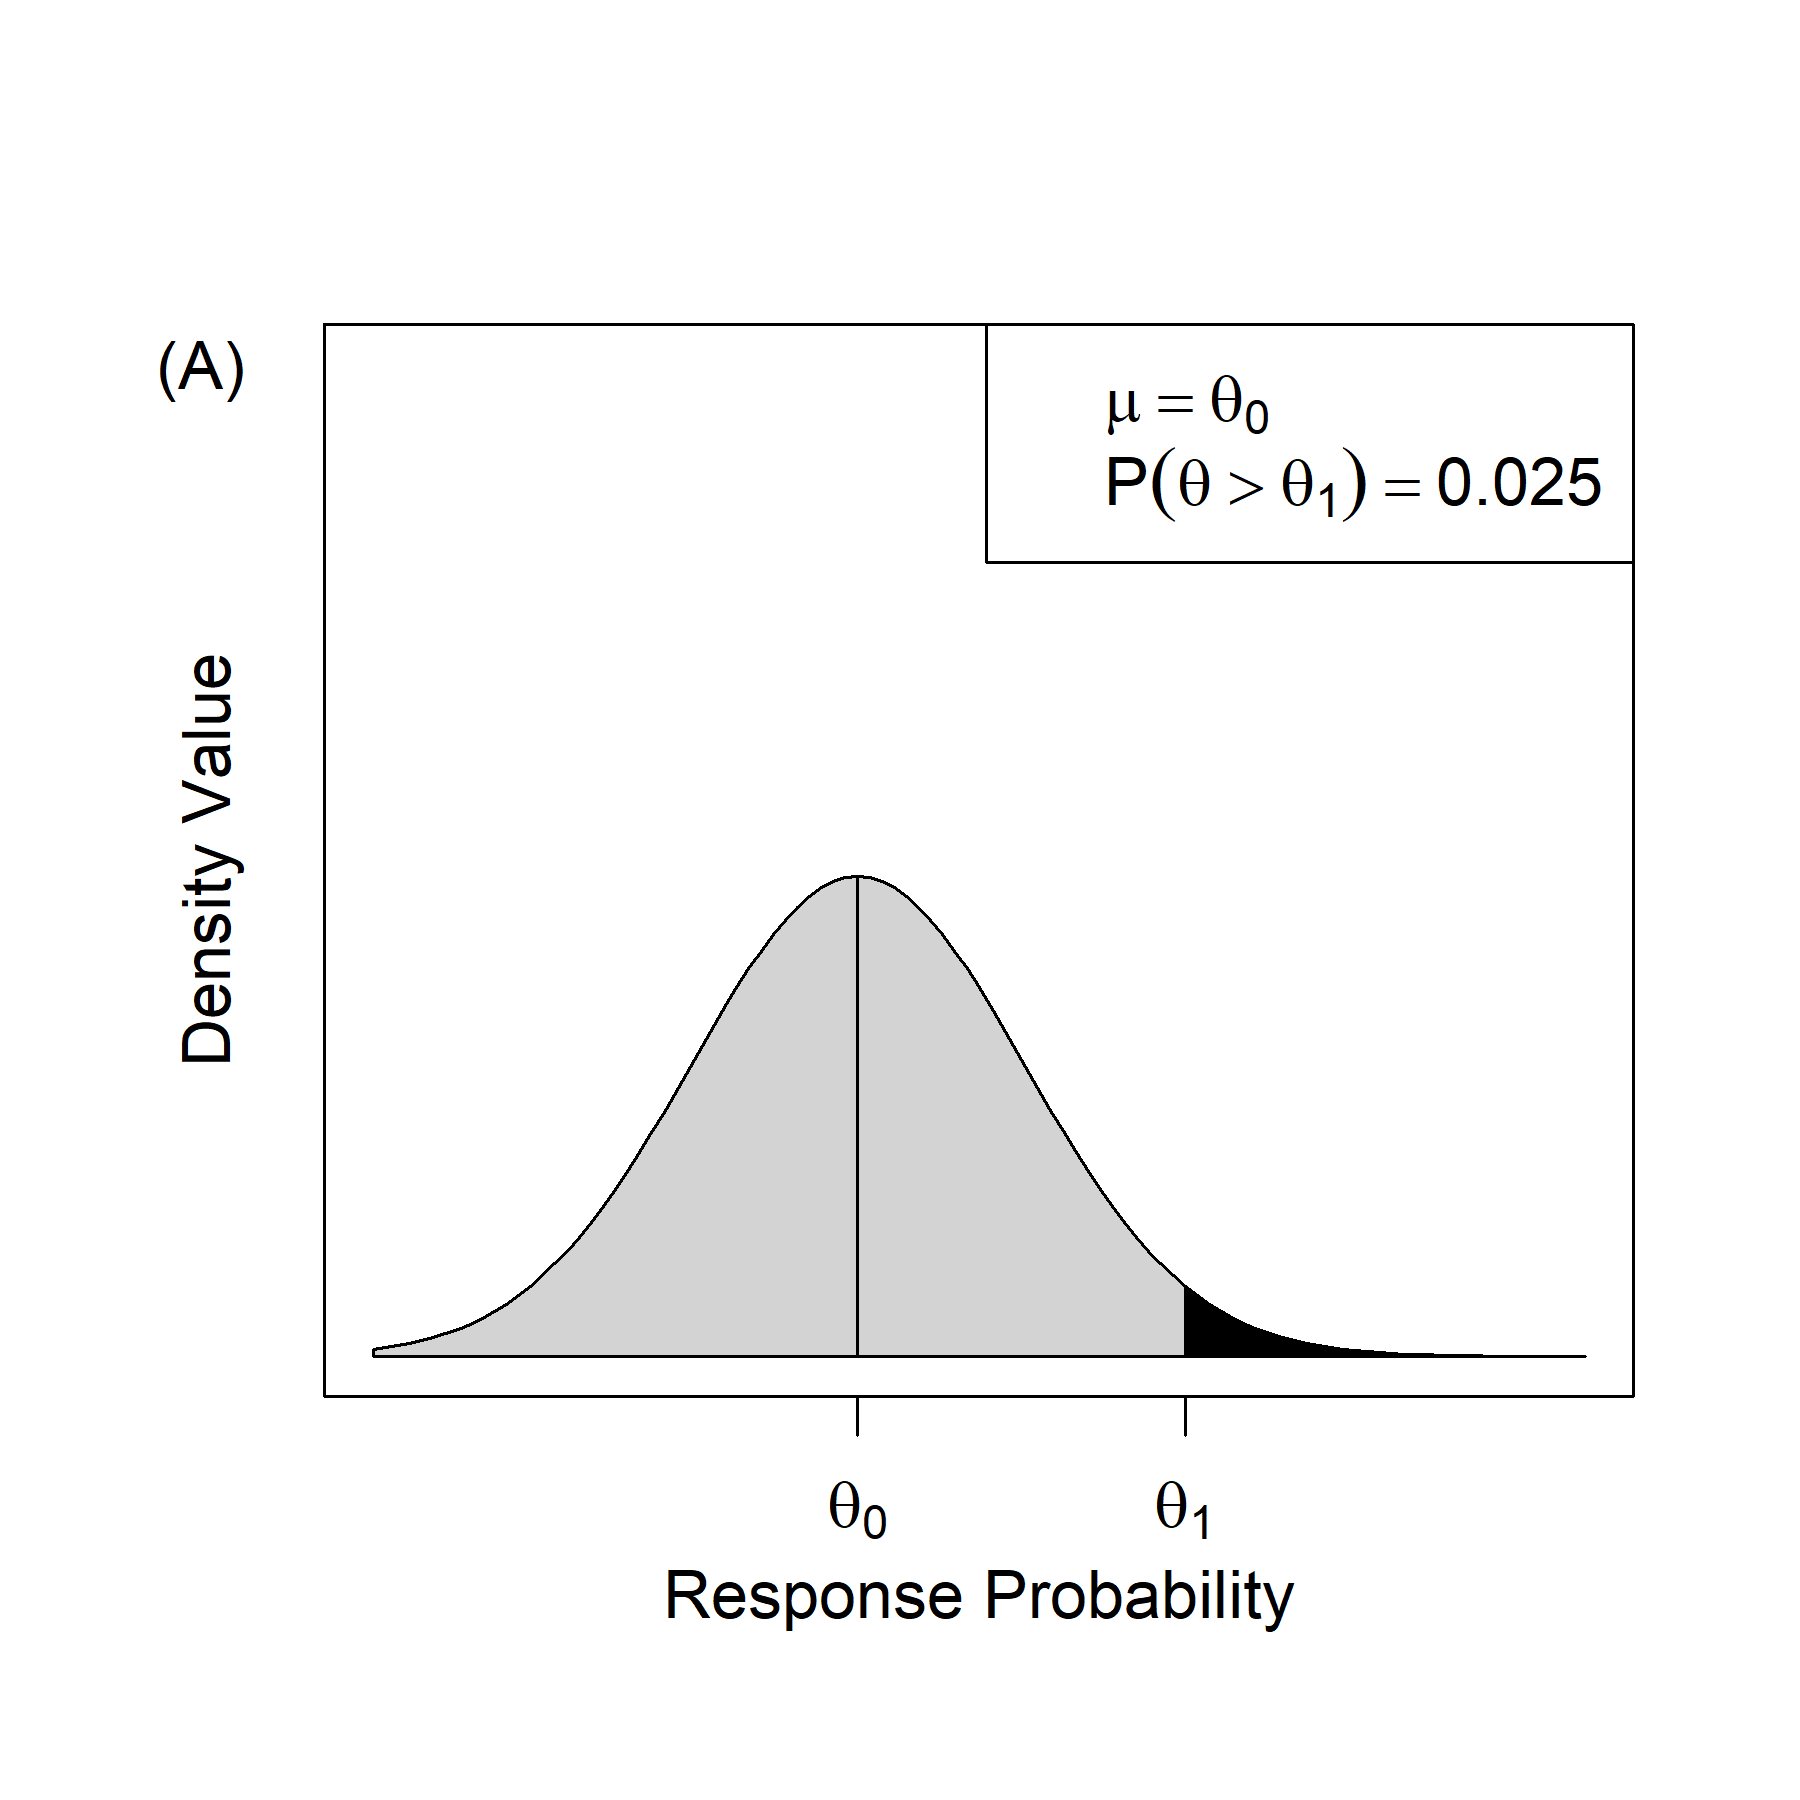
\includegraphics[width=3in]{./FIGURES/figure1a.png}
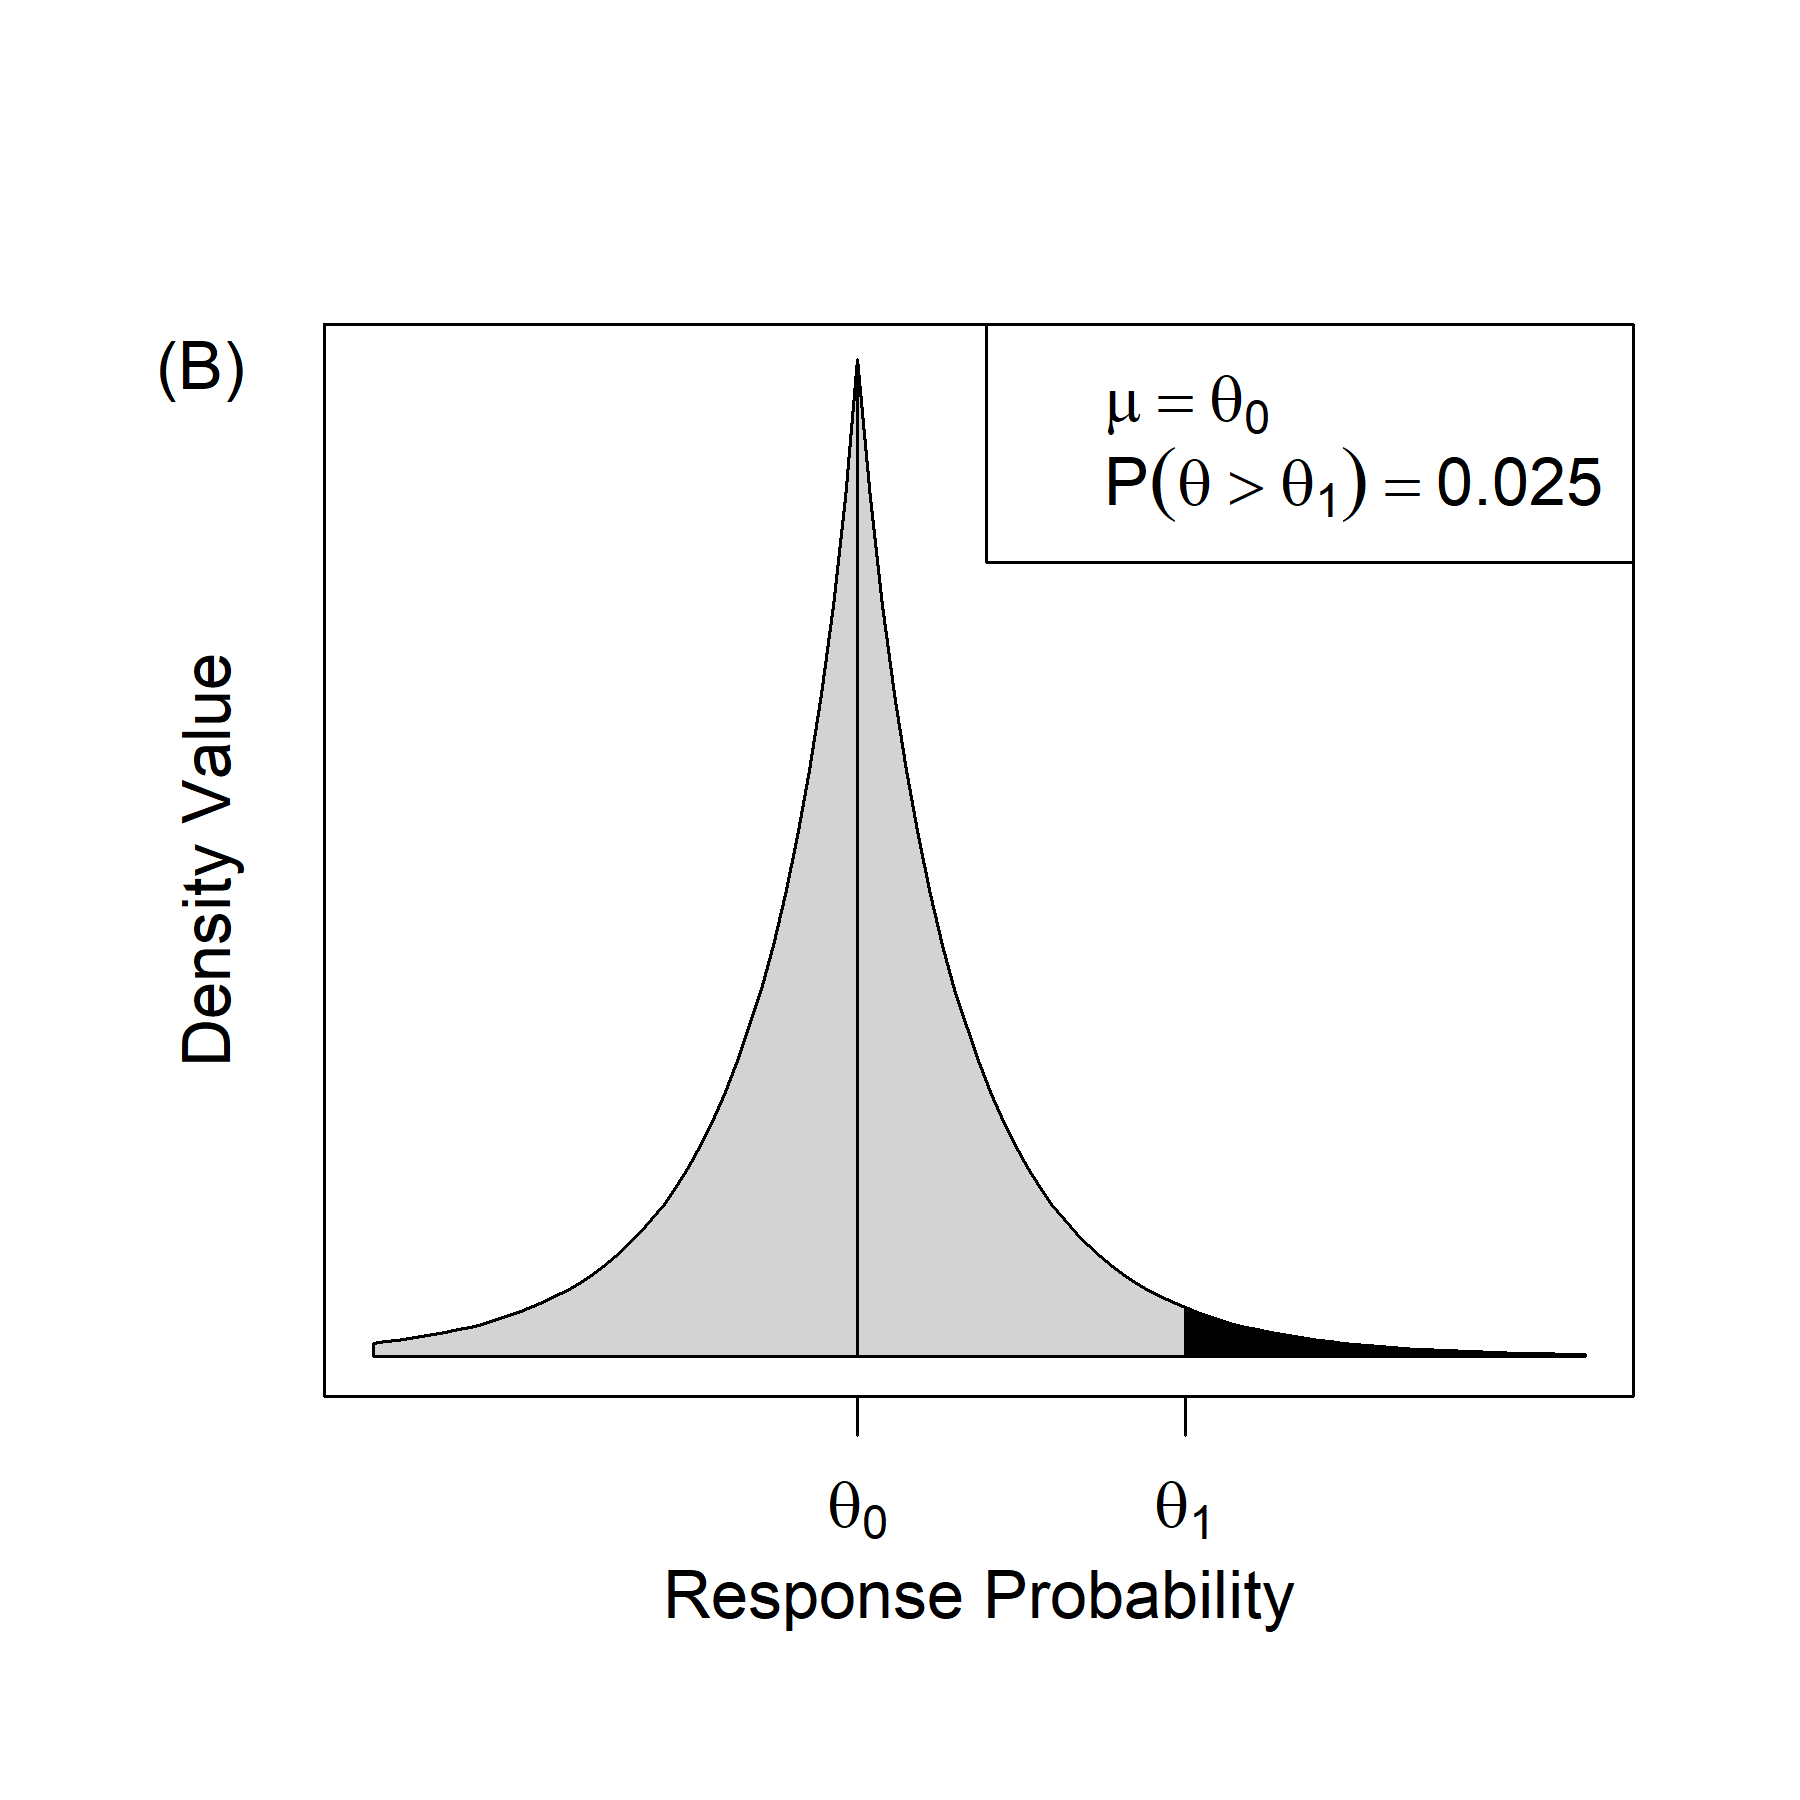
\includegraphics[width=3in]{./FIGURES/figure1b.png}

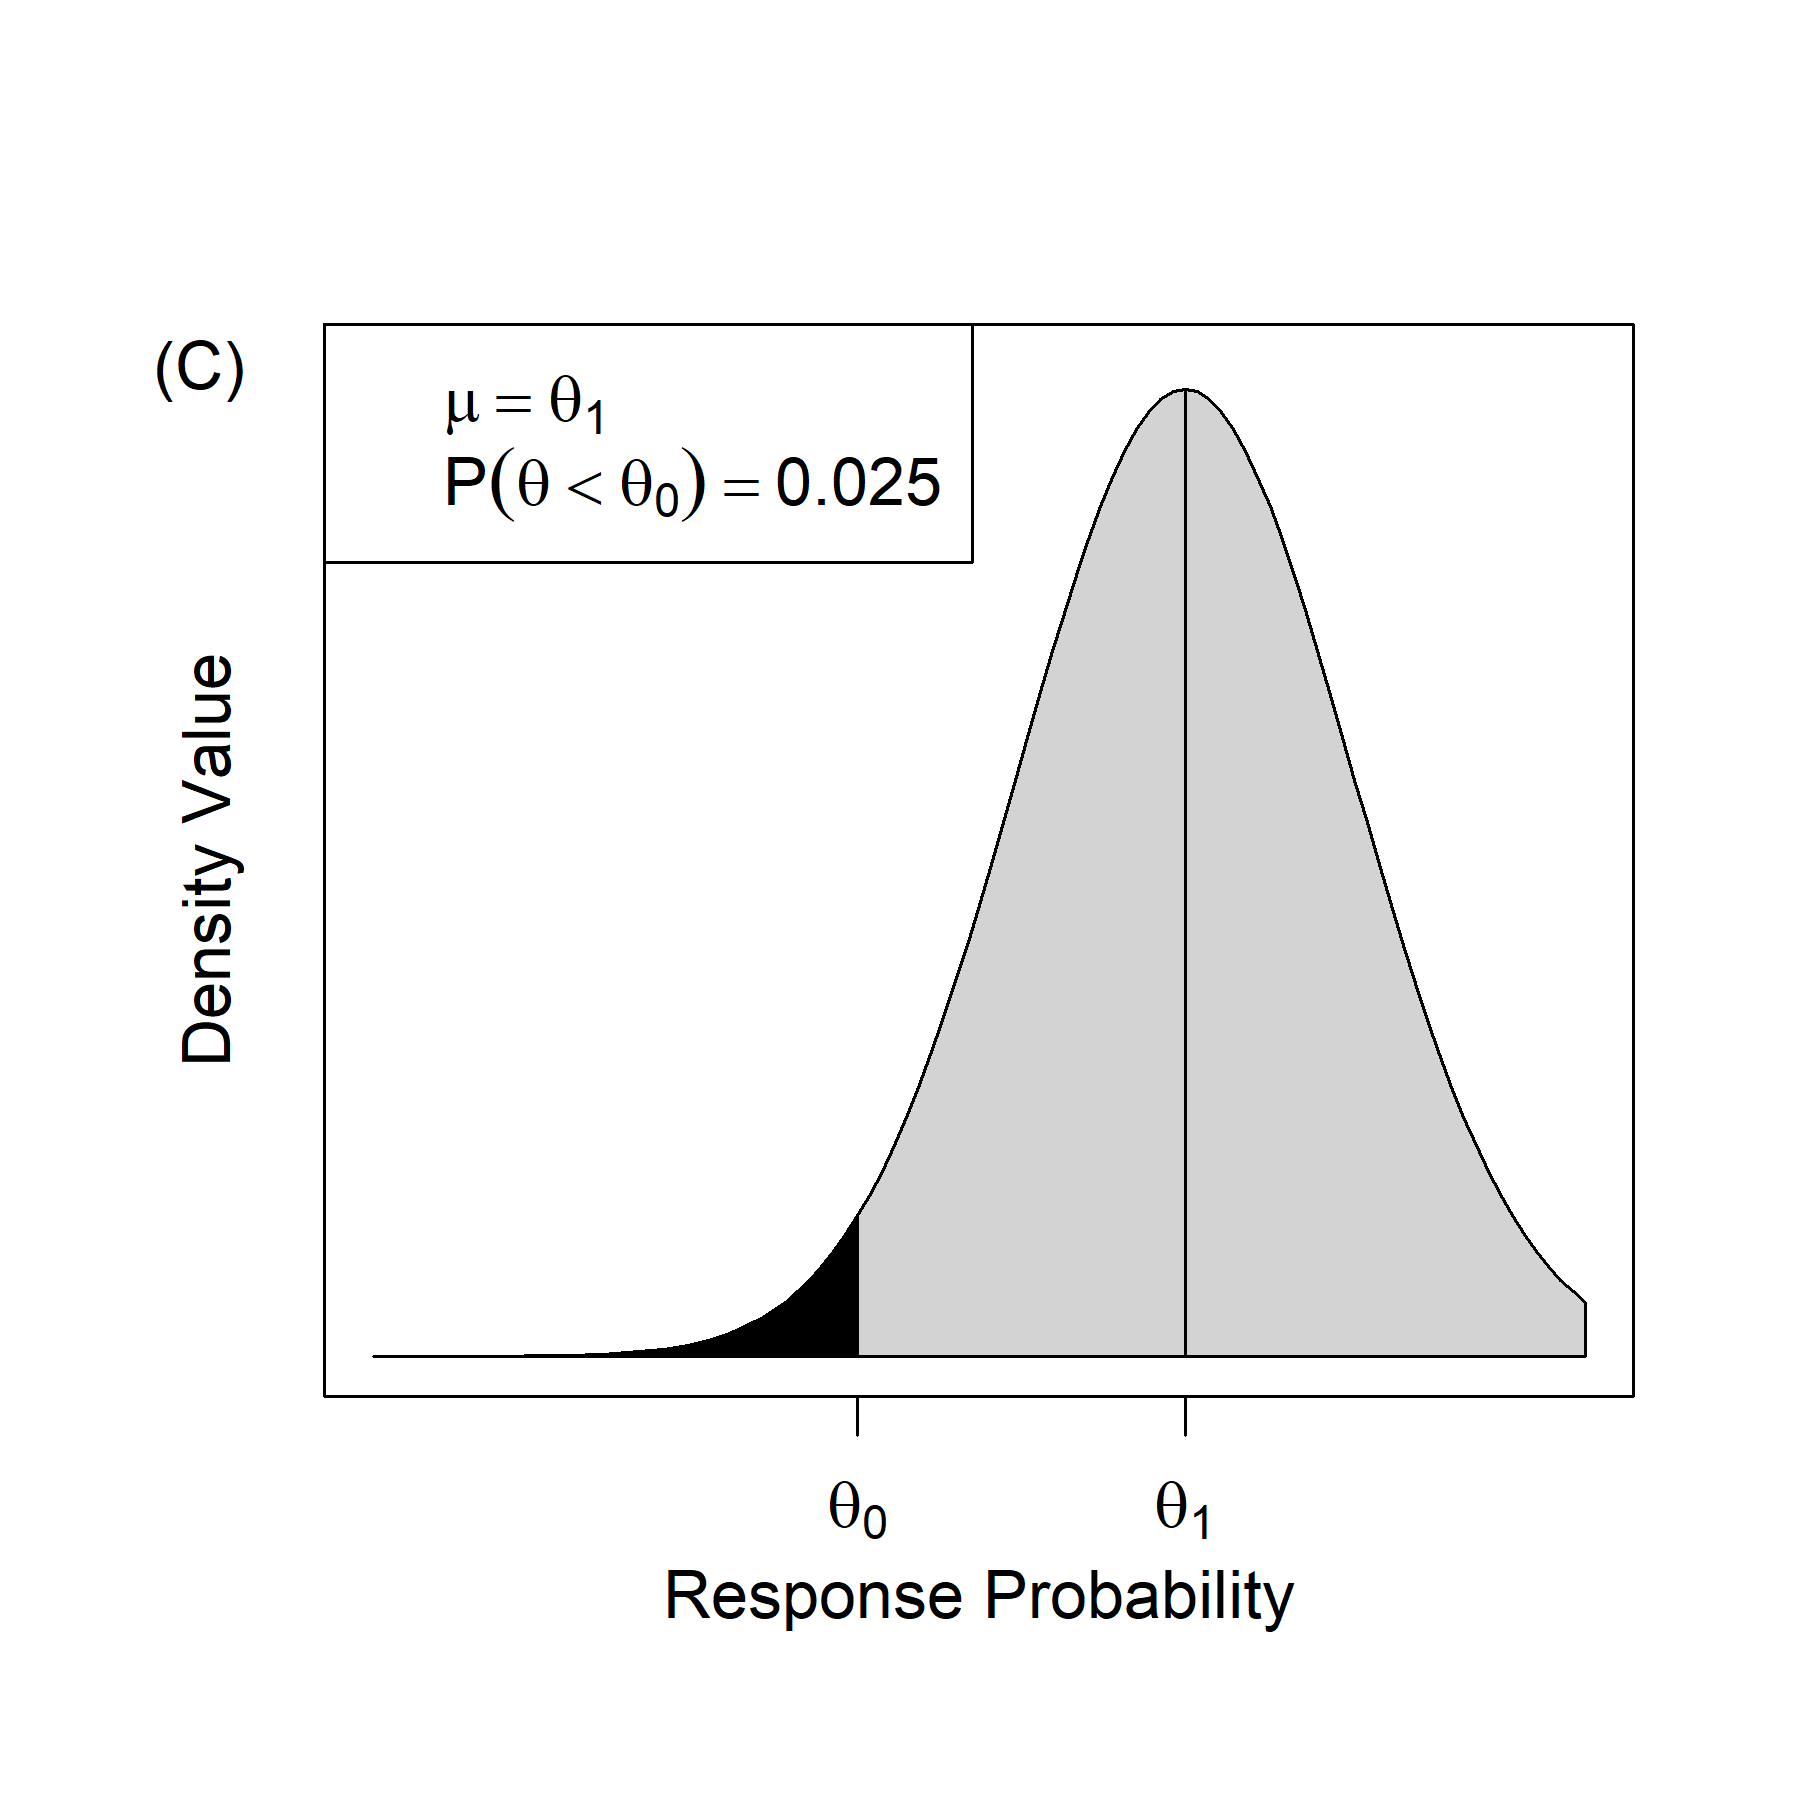
\includegraphics[width=3in]{./FIGURES/figure1c.png}
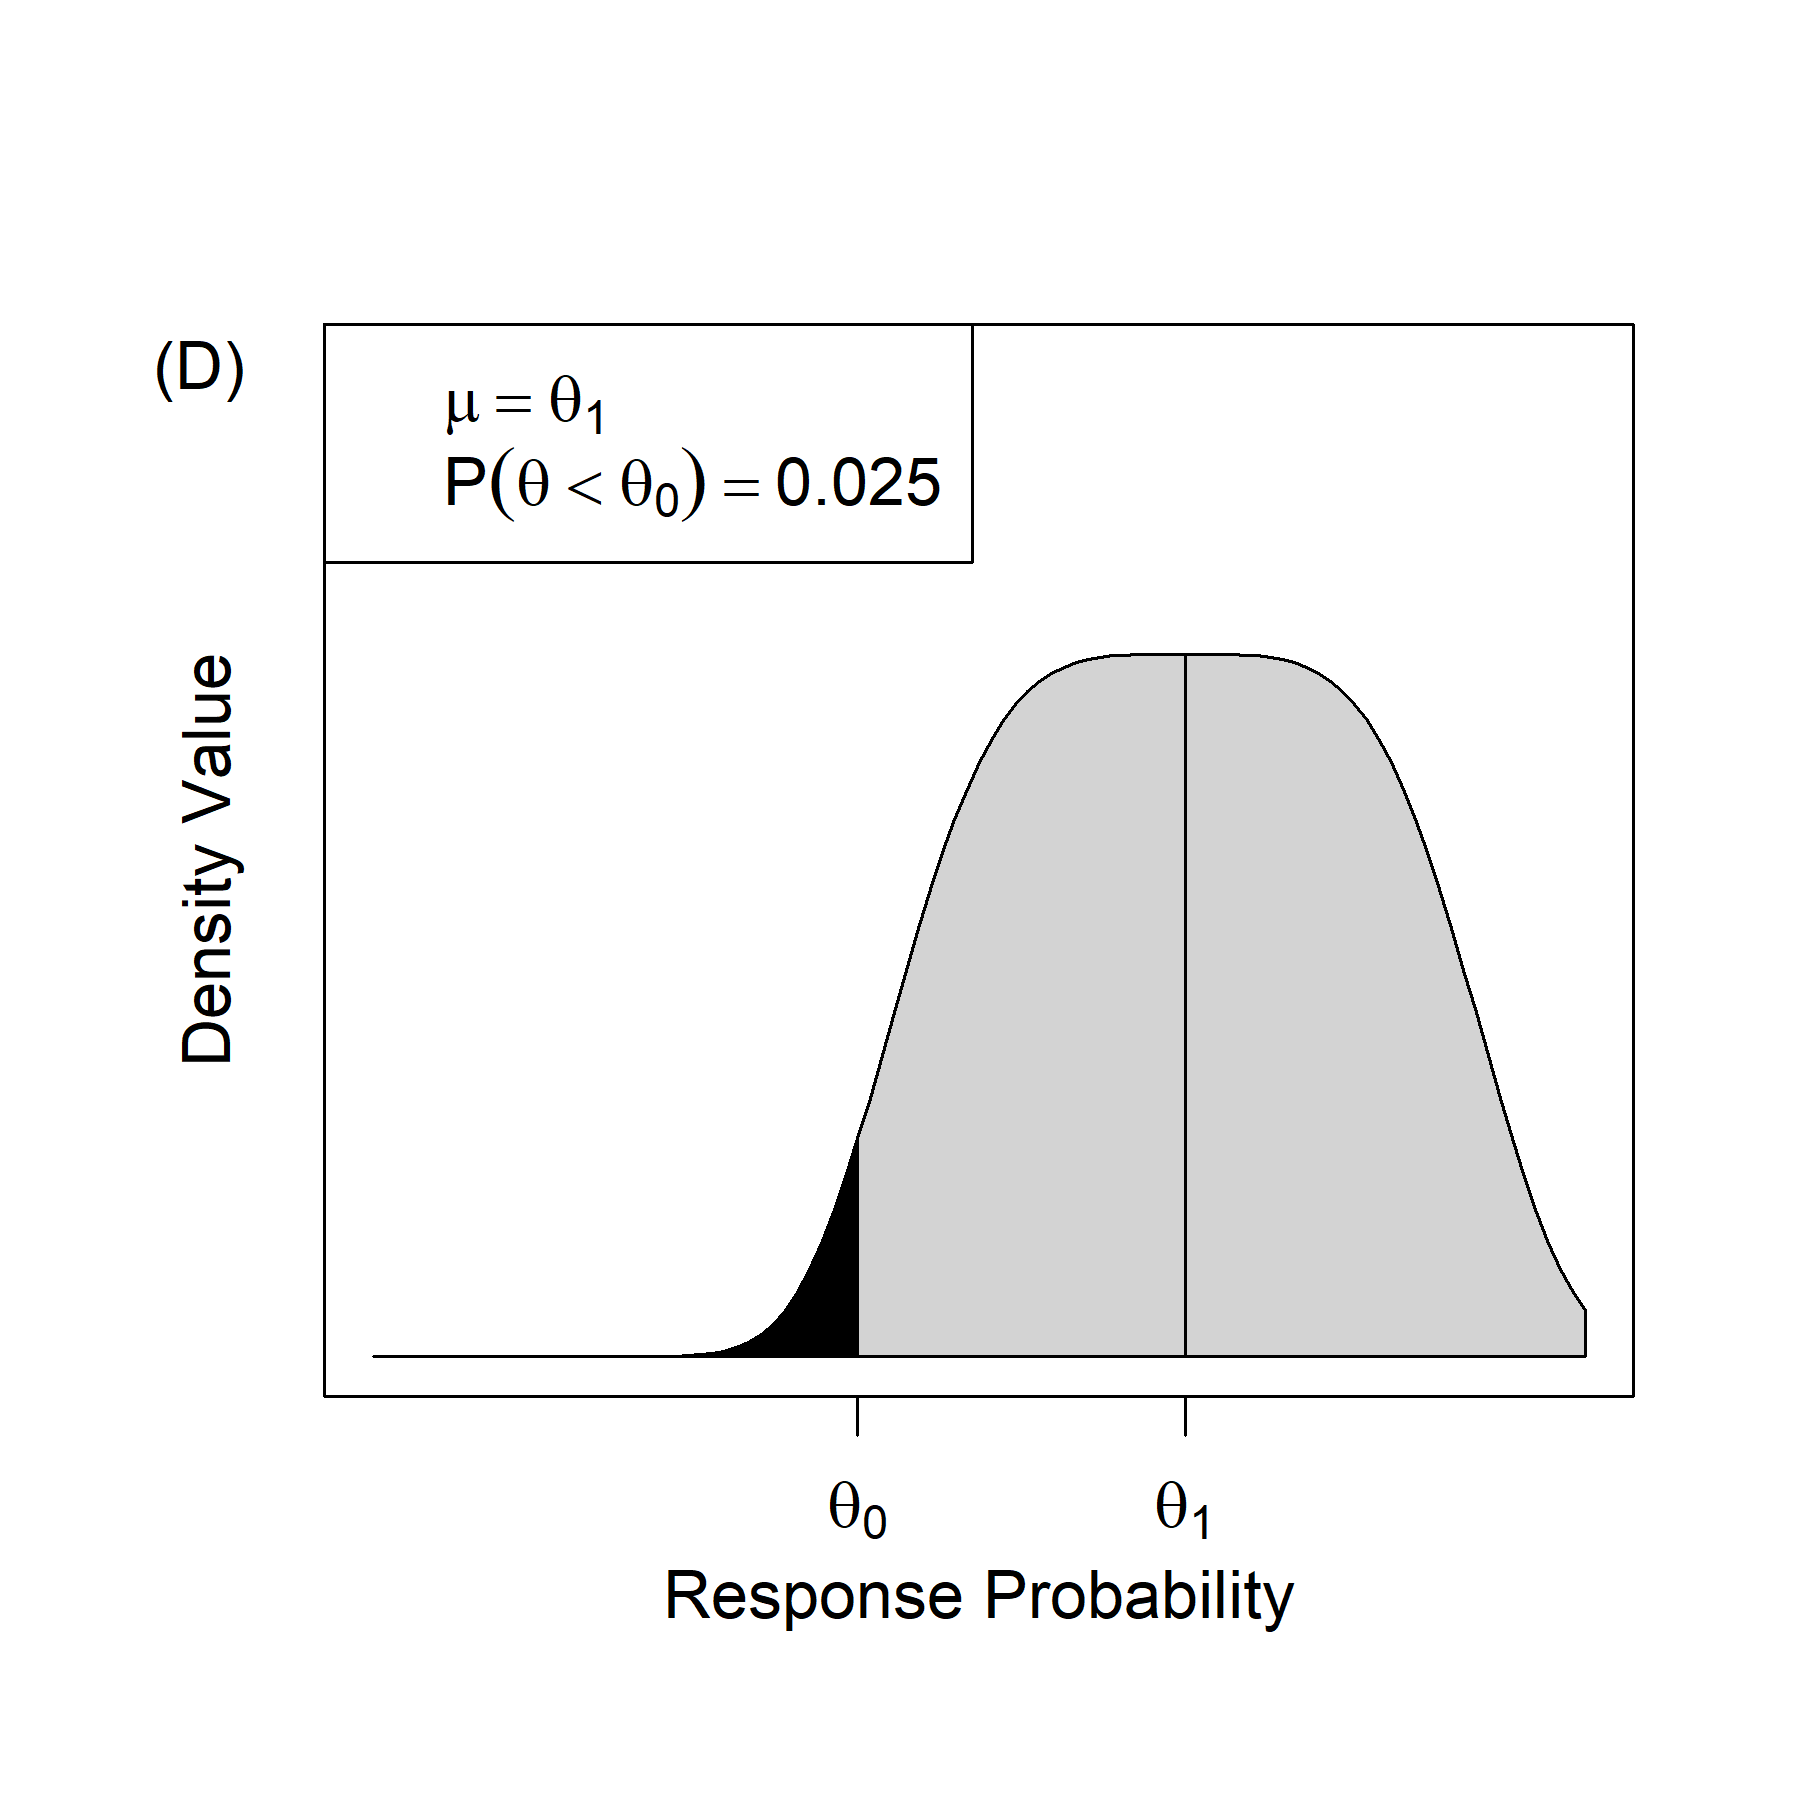
\includegraphics[width=3in]{./FIGURES/figure1d.png}

\caption{A, Skeptical prior, normal distribution. B, Skeptical prior, generalized normal distribution with added concentration around modal value. C, Enthusiastic prior, normal distribution. D, Enthusiastic prior, generalized normal distribution with added flattening around modal value.}
\label{fig:figure1}
\end{center}\end{figure}
\subsubsection{One Arm Example}
The default skeptical and enthusiastic priors will be of the form \eqref{eq:generalizednormalkernel} and are truncated to the unit interval. 
\begin{align}
\pi_S(\theta)&=c_S \exp\left\{-\frac{|\theta-\theta_0|}{\alpha_S}^{\beta_S}\right\}{I(\theta\in[0,1])} \label{eq:ex1skptprior}\\
\pi_E(\theta)&=c_E\exp\left\{-\frac{|\theta-\theta_1|}{\alpha_E}^{\beta_E}\right\}{I(\theta\in[0,1])}\label{eq:ex1enthprior}
\end{align}
where $c_S=\frac{\beta_S}{2\alpha_S \Gamma(1/\beta_S)({F_{\theta_0,\alpha_S,\beta_S}(1)-F_{\theta_0,\alpha_S,\beta_S}(0)})}$ and $c_E=\frac{\beta_E}{2\alpha_E \Gamma(1/\beta_E)({F_{\theta_1,\alpha_E,\beta_E}(1)-F_{\theta_1,\alpha_E,\beta_E}(0)})}$. The values $\beta_S$ and $\beta_E$ are pre-specified and $\alpha_S$ and $\alpha_E$ are chosen to satisfy the tail-probability conditions 
\eqref{eq:enthprior}-\eqref{eq:skptprior}.
%The normal and generalized normal family of distributions can be truncated to a restricted domain that reflects the research quantity of interest (e.g. a response probability on [0,1]).
\subsubsection{Application to higher dimensions}
%Suppose the trial from Section \ref{sec:preliminaries} has added a control arm, and let $\eta_0$ and $\eta_1$ be the response proportions for a control and treatment group respectively. Suppose that the risk difference $\theta=\eta_1-\eta_0$ is the parameter of interest, and let $\eta_0$ be a nuisance parameter. Let $\delta_0$ denote a null risk difference and $\delta_1$ denote a highly efficacious risk difference.

The generalized normal distribution can be used to parameterize skeptical and enthusiastic priors for trials with multiple unknown quantities of interest. Let $\theta$ be the parameter of interest and $\eta$ be the nuisance parameters. Consider the following representation of the joint prior for $\theta$ and $\eta$:
\begin{align}
\pi(\theta,\eta)=&\pi(\theta)\times\pi(\eta|\theta). \label{eq:generalized_normal_joint}
\end{align}

Each of these components can be represented in the form of \eqref{eq:generalizednormalkernel} by
\begin{align}
\pi(\theta)&\sim\mathcal{GN}(\mu_\theta,\alpha_\theta,\beta_\theta) \label{eq:genNormPlacebo}\\
\pi(\eta|\theta)&\sim\mathcal{GN}(\mu_\eta,\alpha_\eta,\beta_\eta) \label{eq:genNormRd}
\end{align}

\subsubsection{Example: 2 arm risk difference}

The priors will be chosen based on the generalized normal distribution \eqref{eq:generalizednormalkernel} based on the joint specification in \eqref{eq:generalized_normal_joint} and truncated to the domain of a difference in response proportion $(-1, 1)$.

\begin{align*}
\pi_S(\theta)&=c_S \exp\left\{-\frac{|\theta-\theta_0|}{\alpha_S}^{\beta_S}\right\}{I(\theta\in[-1,1])}\\
\pi_E(\theta)&=c_E\exp\left\{-\frac{|\theta-\theta_1|}{\alpha_E}^{\beta_E}\right\}{I(\theta\in[-1,1])}
\end{align*}
where $c_S=\frac{\beta_S}{2\alpha_S \Gamma(1/\beta_S)({F_{\theta_0,\alpha_S,\beta_S}(1)-F_{\theta_0,\alpha_S,\beta_S}(-1)})}$ and $c_E=\frac{\beta_E}{2\alpha_E \Gamma(1/\beta_E)({F_{\theta_1,\alpha_E,\beta_E}(1)-F_{\theta_1,\alpha_E,\beta_E}(-1)})}$. The values $\beta_S$ and $\beta_E$ are pre-specified and $\alpha_S$ and $\alpha_E$ are chosen to satisfy the tail-probability conditions 
\eqref{eq:enthprior}-\eqref{eq:skptprior}.

The skeptical and enthusiastic priors will have the same component for $\pi(\eta|\theta)$ which is truncated to $[0,1-\theta)$ if $\theta\geq 0$ and $(-\theta,1)$ if $\theta < 0$: 
\begin{align*}
\pi(\eta|\theta)=c_\eta\text{exp}\left\{\frac{|\eta-\mu_\eta|^{\beta_\eta}}{\alpha_\eta}\right\}\left(\frac{I(\text{max}(-\theta,0)\leq\eta\leq \text{min}(1,1+\theta))}{F_{\mu_\eta,\alpha_\eta,\beta_\eta}(\text{min}(1,1+\theta))-F_{\mu_\eta,\alpha_\eta,\beta_\eta}(\text{max}(0,-\theta))}\right)
\end{align*}
where $c_\eta=\frac{\beta_\eta}{2\alpha_\eta\Gamma(\beta_\eta)}$. Then the full joint priors are $\pi_S(\theta,\eta)=\pi_S(\theta)\pi(\eta|\theta)$ and $\pi_E(\theta,\eta)=\pi_E(\theta)\pi(\eta|\theta)$.
Section \ref{sec:example2model} uses this representation of the joint prior.
%The component $\pi(\theta_0)$ reflects prior opinion about the response rate in the placebo group, and the component $\pi(\theta_1|\theta_0)$ can be used to express pessimism or optimism in the difference in proportions $\theta_1 - \theta_0$. 
%
%The enthusiastic prior condition from \eqref{eq:enthprior} become
%\begin{align}\label{eq:ex2enthcondition}
%P(\theta_1-\theta_0>\delta_0)=1-\epsilon.
%\end{align}
%
%The skeptical prior condition from \eqref{eq:skptprior} become
%\begin{align}\label{eq:ex2skptcondition}
%P(\theta_1-\theta_0<\delta_1)=1-\epsilon.
%\end{align}

\begin{figure}\begin{center}
%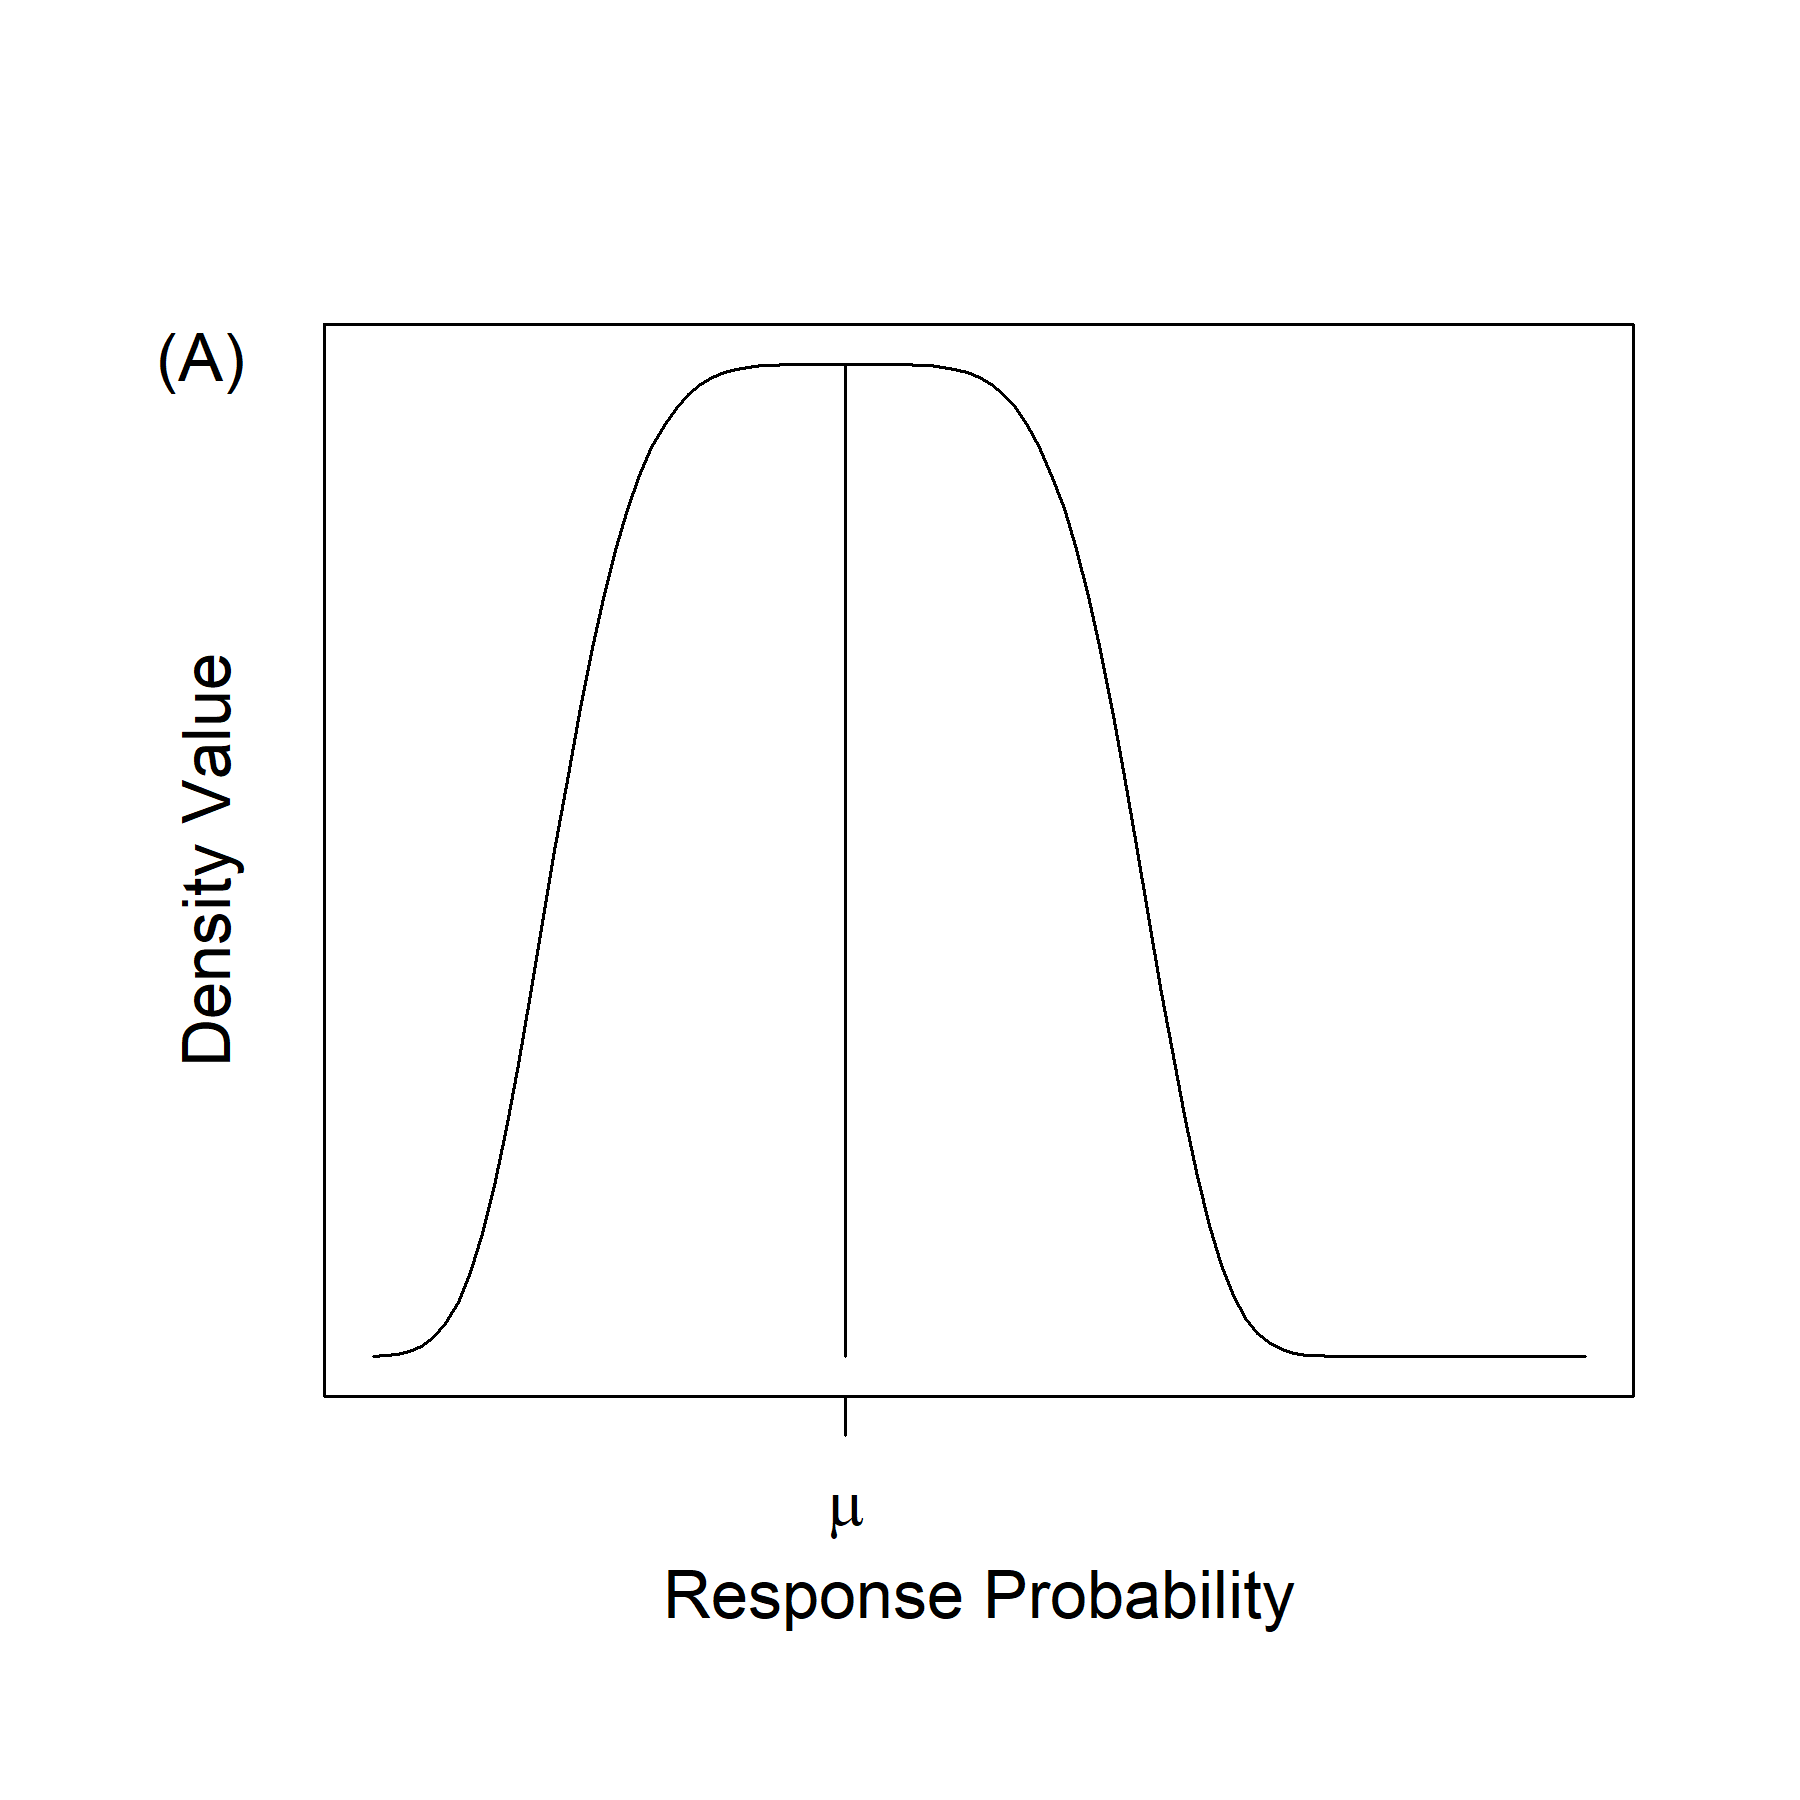
\includegraphics[width=3in]{./FIGURES/figure5c.png}

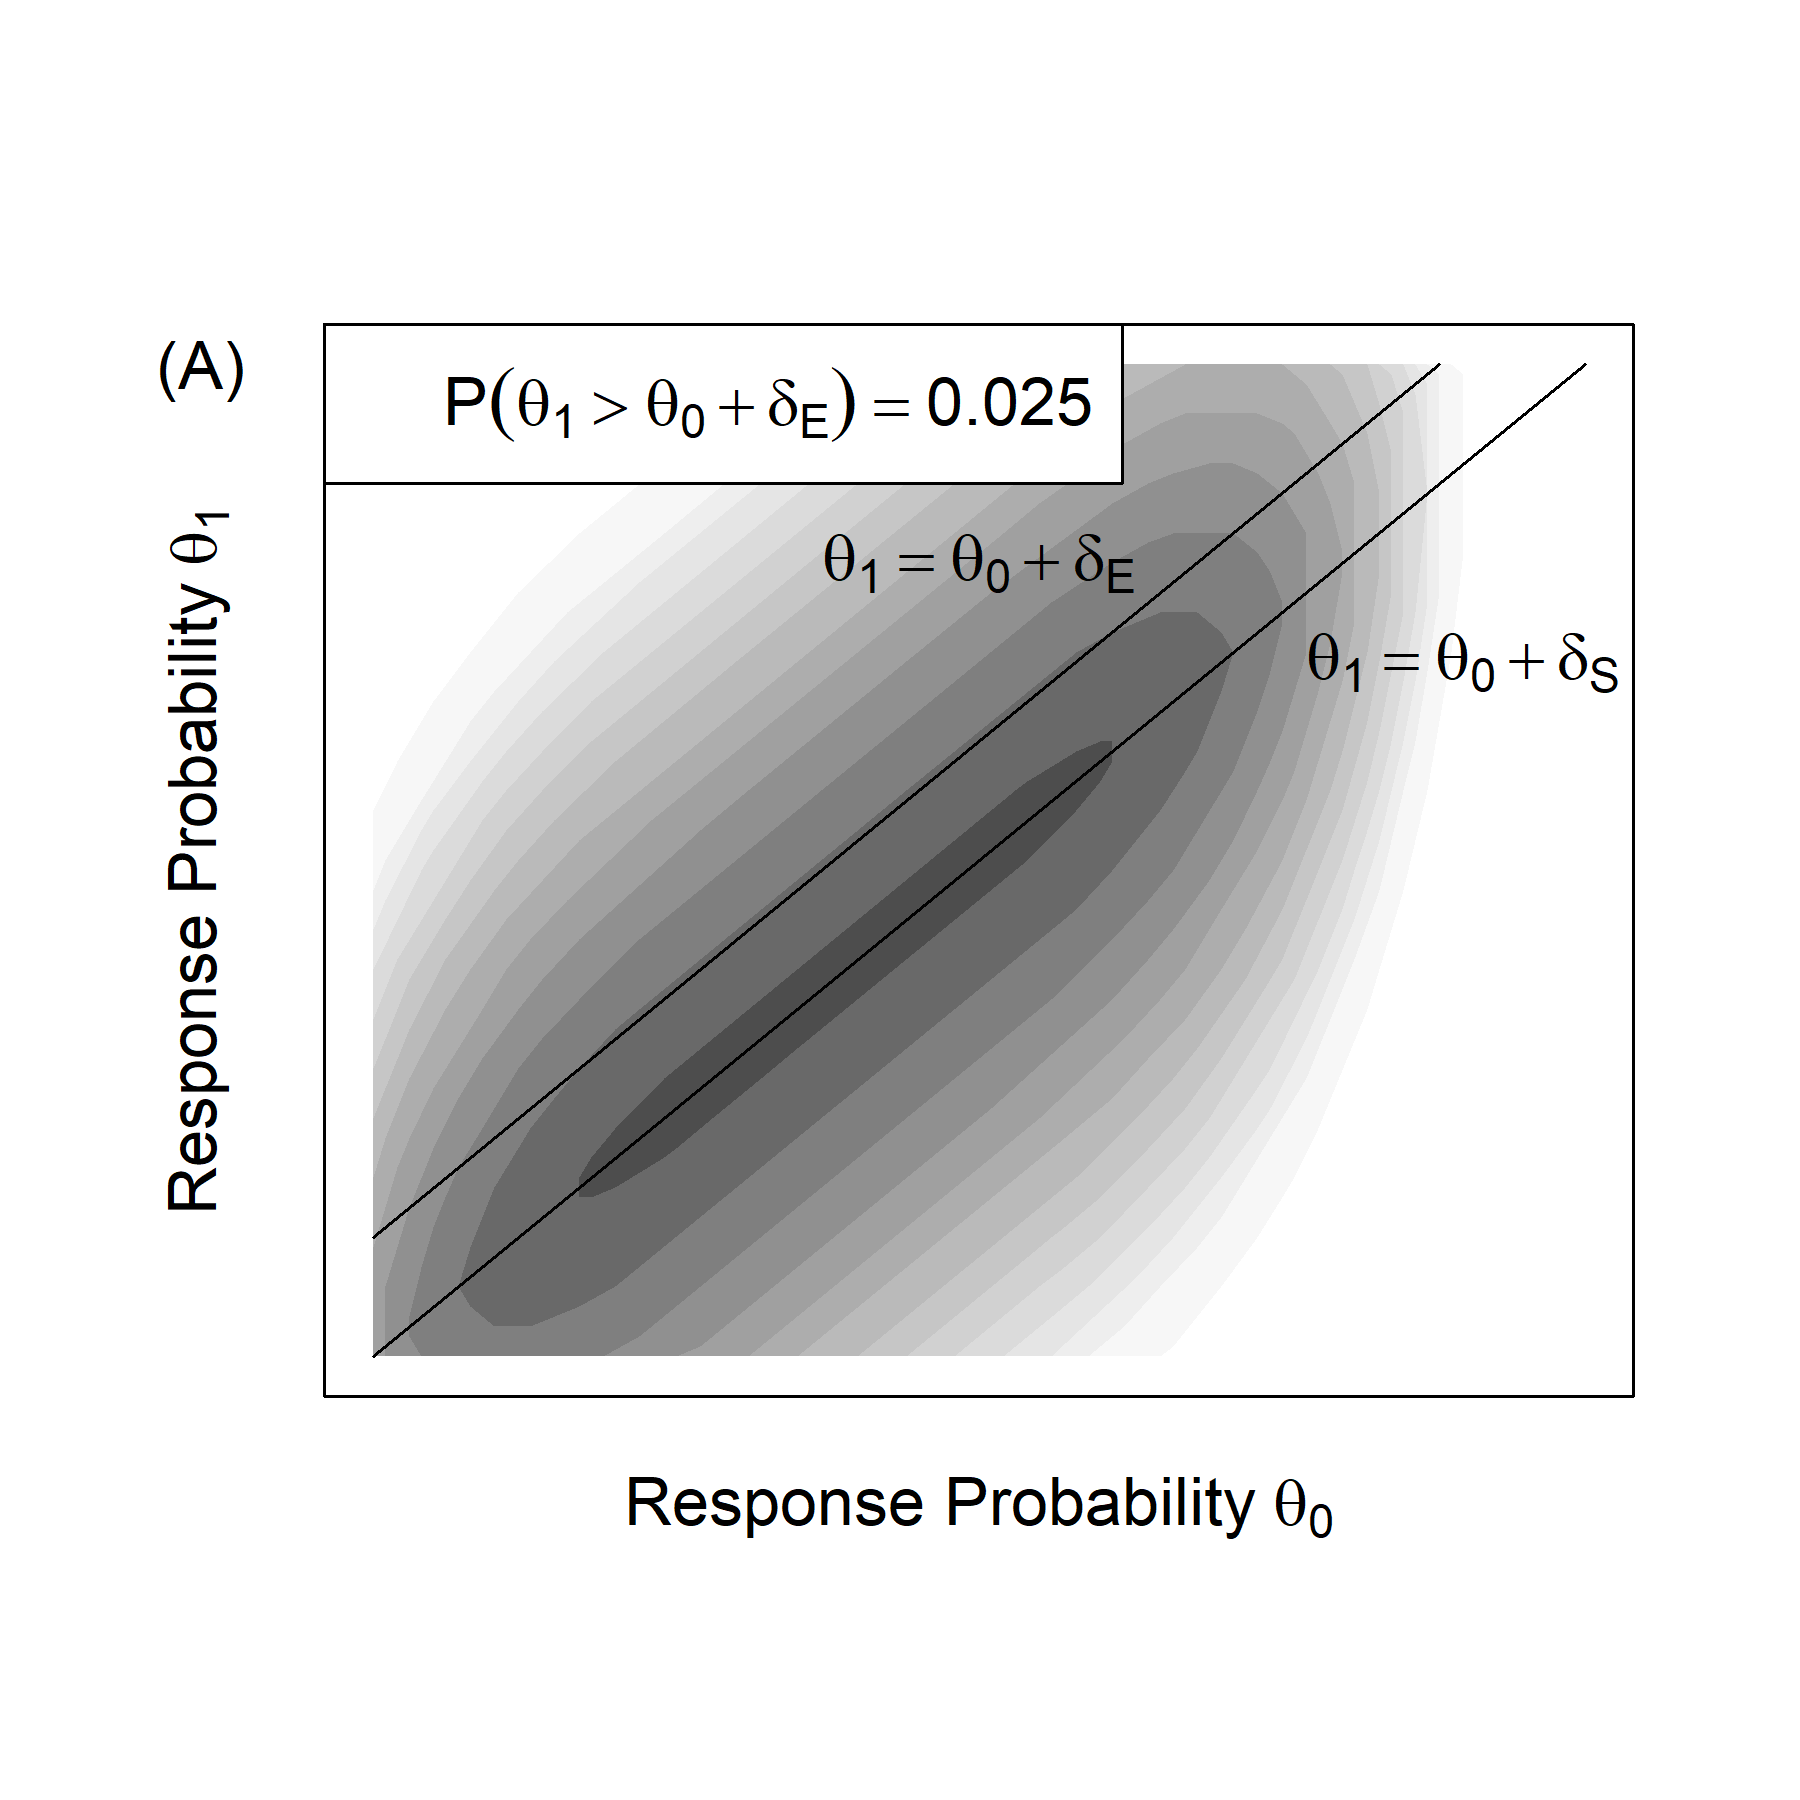
\includegraphics[width=3in]{./FIGURES/figure5a.png}
%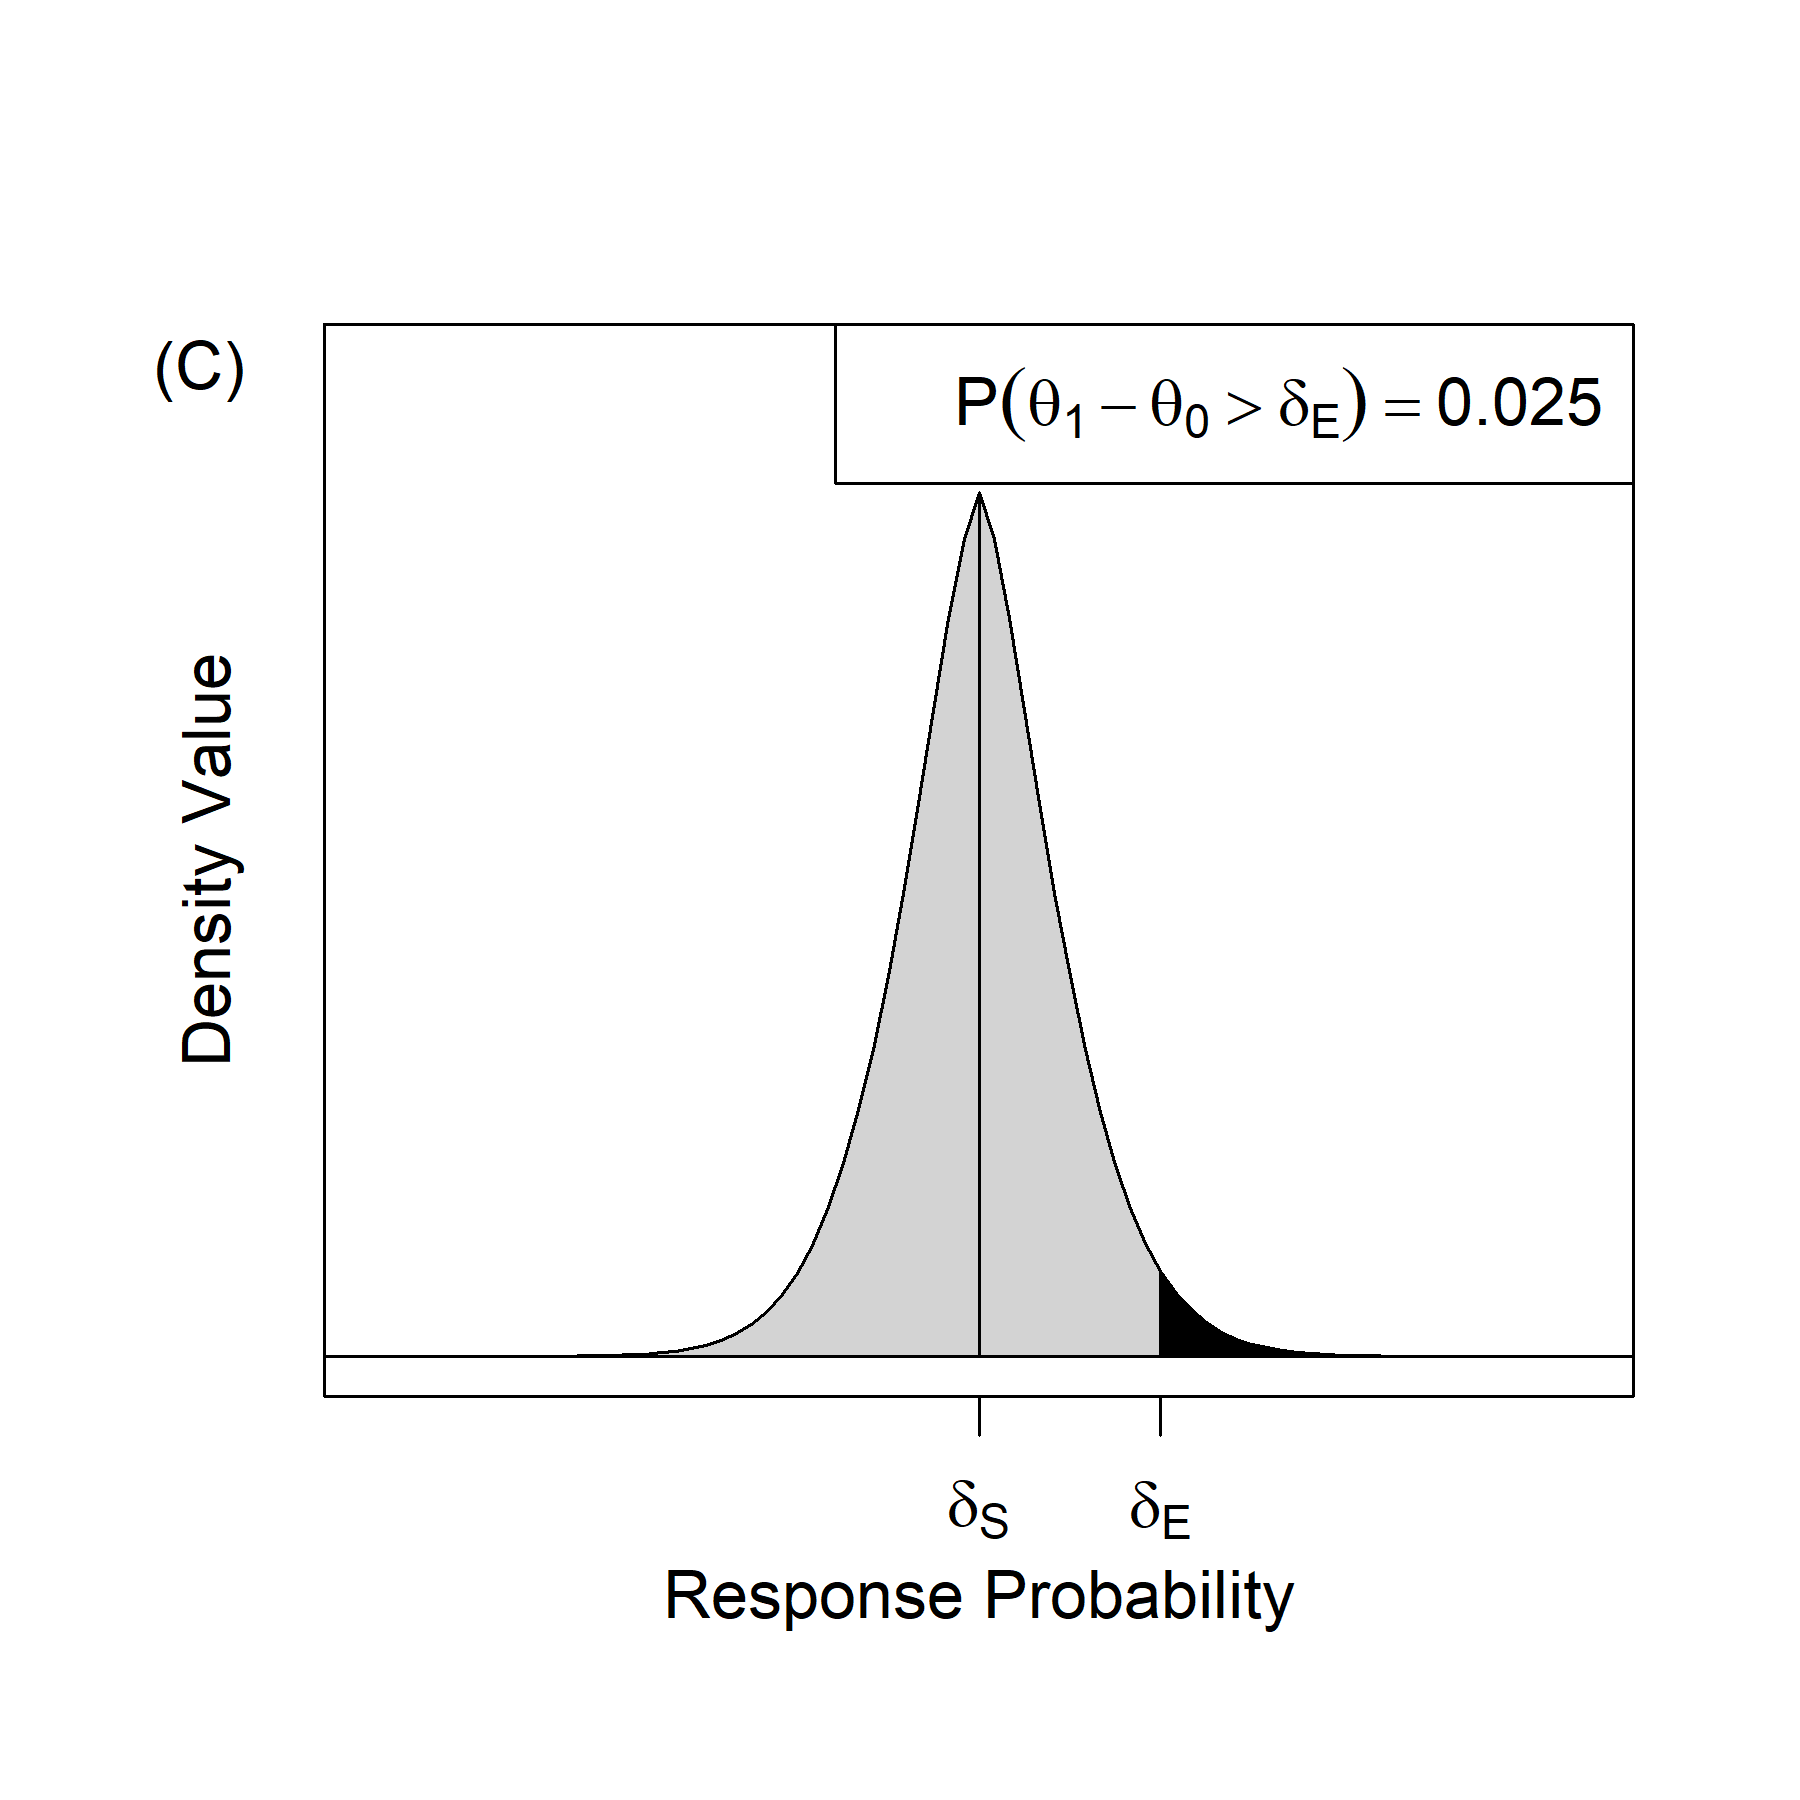
\includegraphics[width=3in]{./FIGURES/figure5d.png}

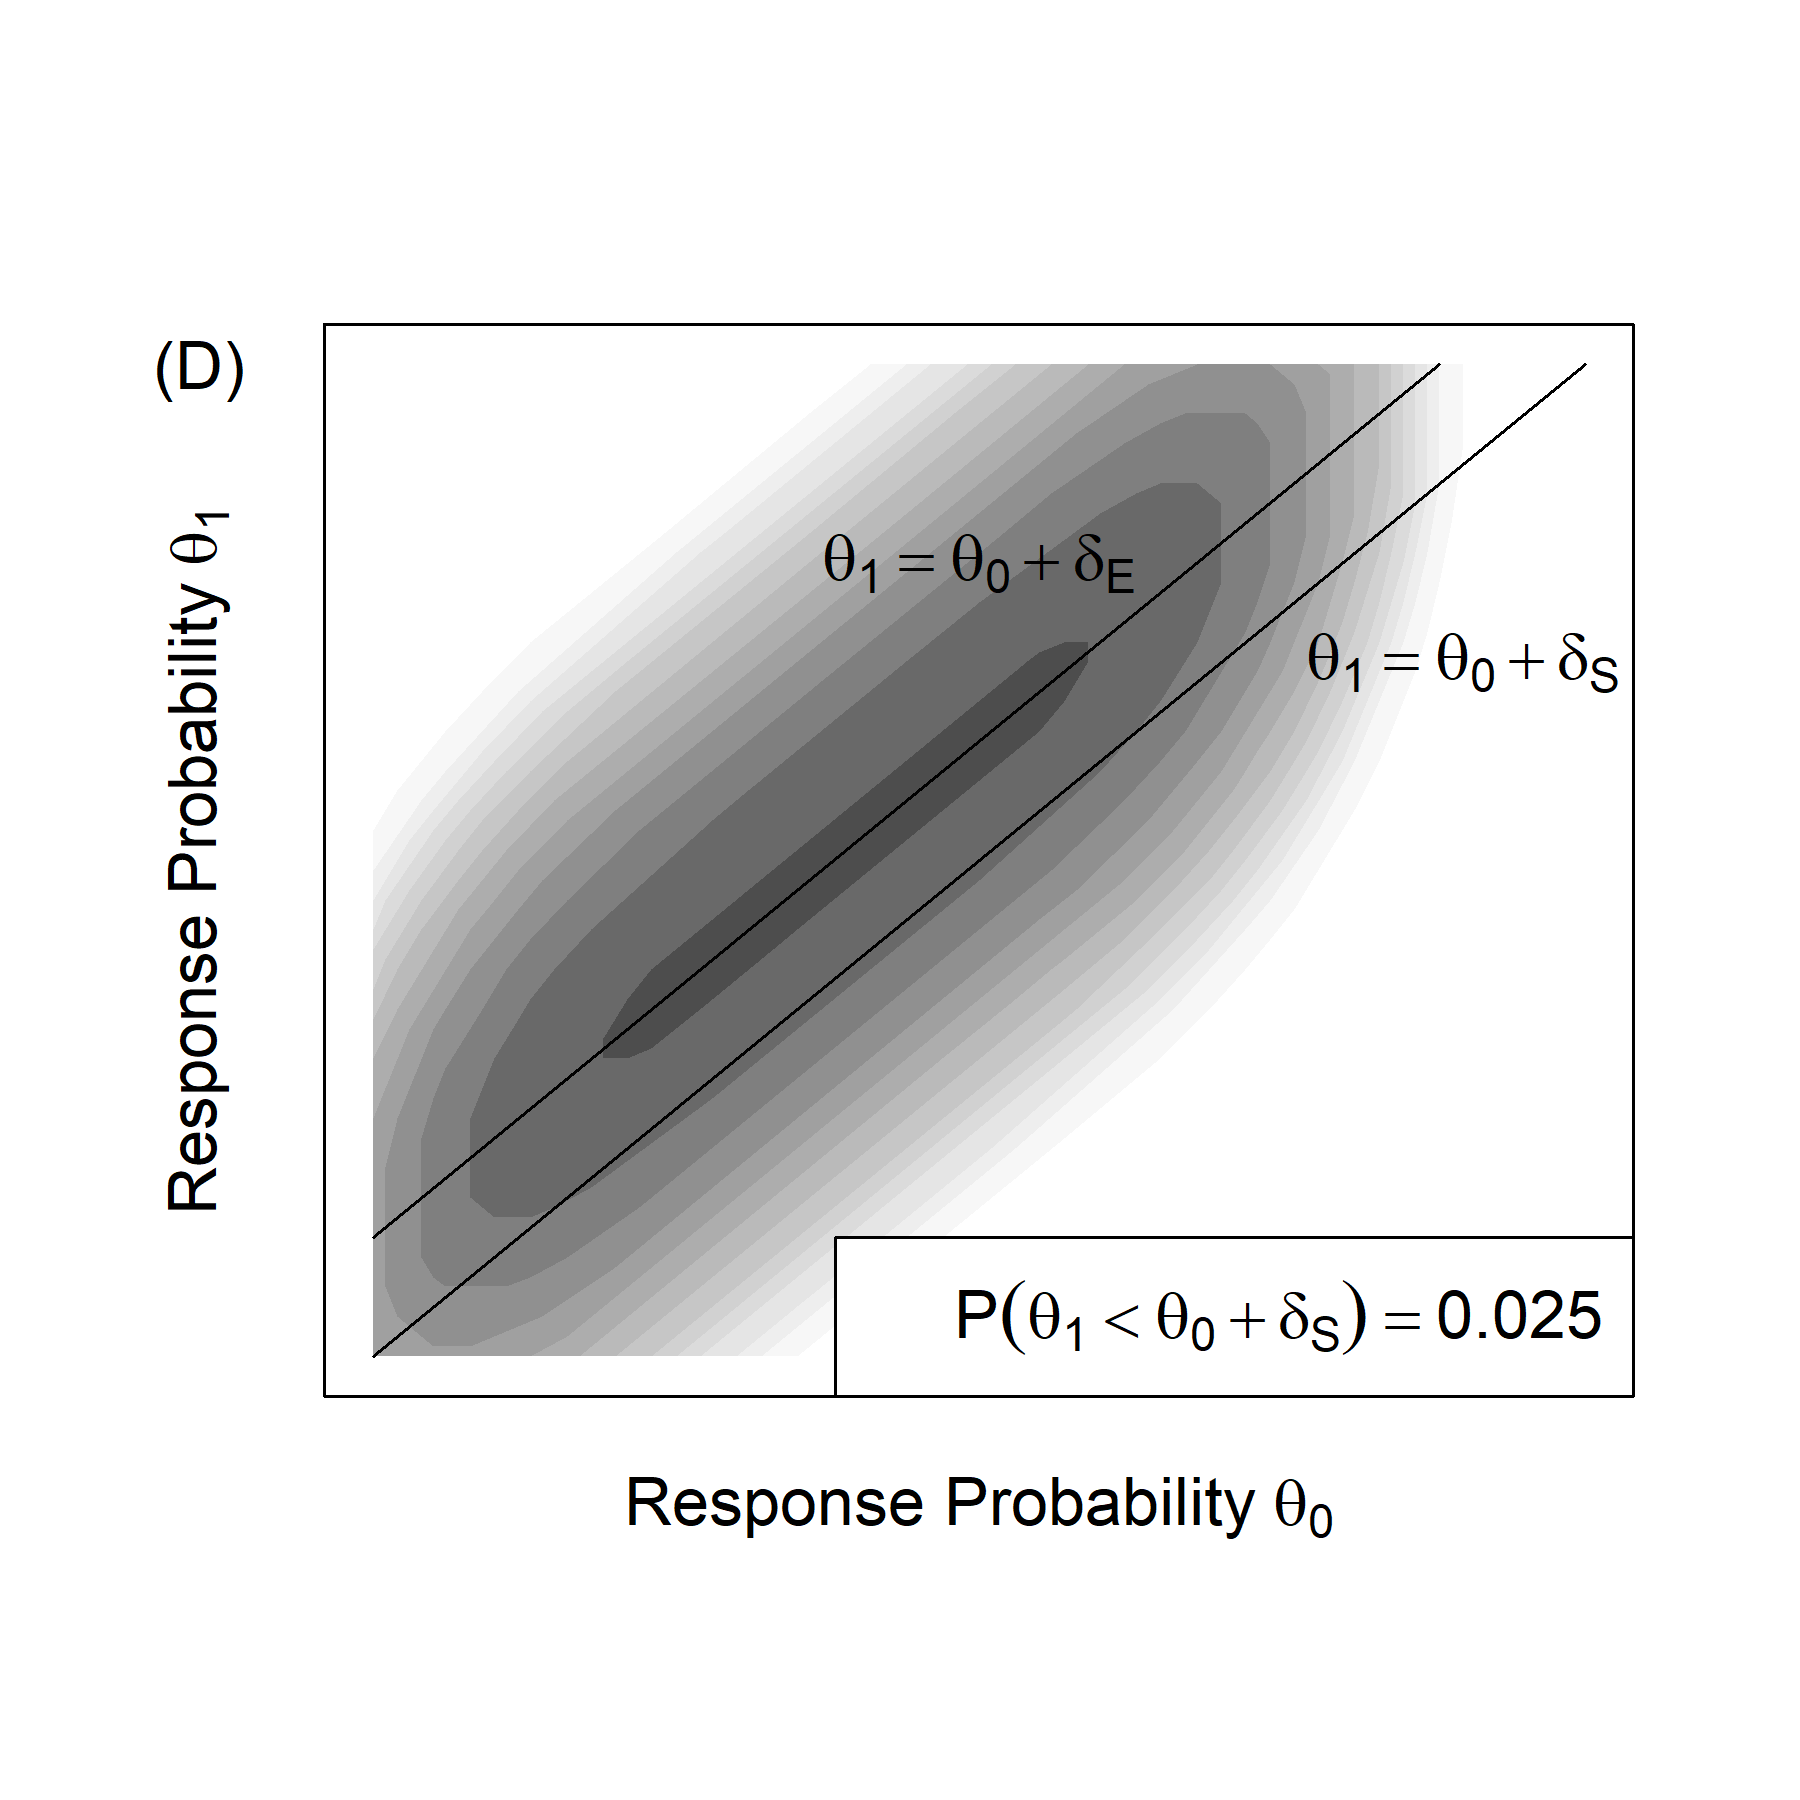
\includegraphics[width=3in]{./FIGURES/figure5b.png}
%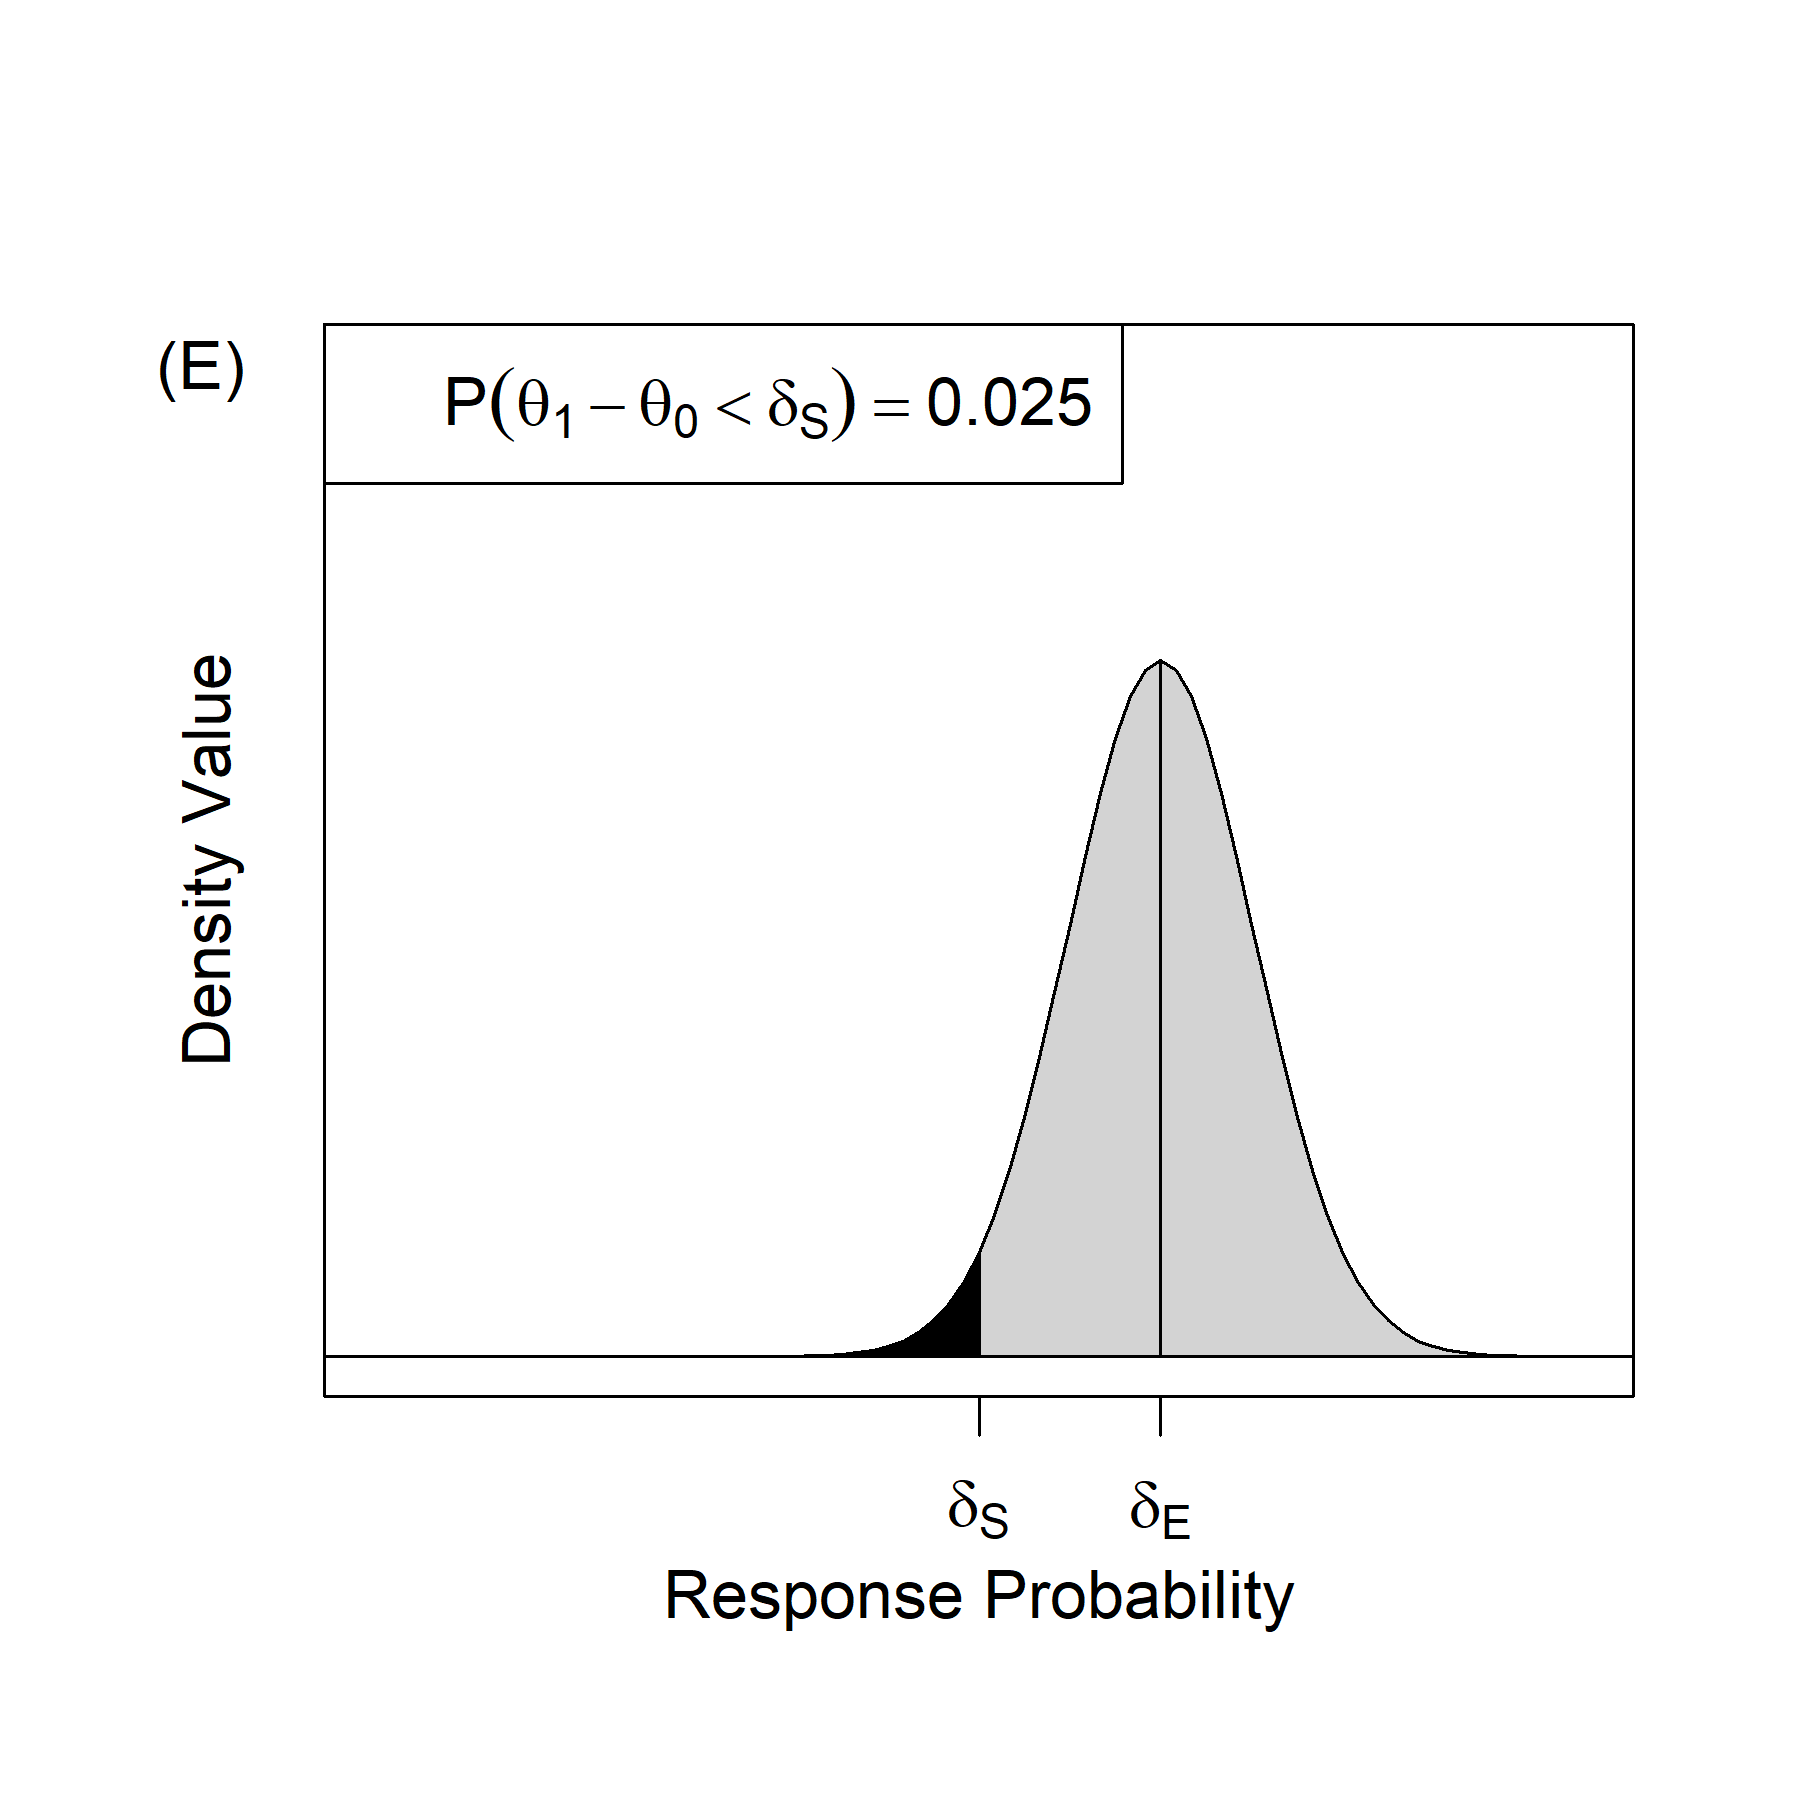
\includegraphics[width=3in]{./FIGURES/figure5e.png}
\caption{A, Univariate prior $\pi(\theta_0)$. B, Skeptical joint prior $\pi_S(\theta_0,\theta_1)$. C, Skeptical marginal prior $\pi_S(\theta_1-\theta_0)$. D, Enthusiastic joint prior $\pi_E(\theta_0,\theta_1)$. E, Enthusiastic marginal prior $\pi_E(\theta_1-\theta_0$).}
\label{fig:figure5}
 \end{center}\end{figure}
\subsection{Mixture Inference Priors}
\subsubsection{Definition}
The purpose of the inference prior is to synthesize the posterior inferences from the a priori diverse perspectives to facilitate interpretation of the data once it has been obtained. In this paper we propose using an inference prior that is a combination of the skeptical and enthusiastic priors that were used for monitoring.

The skeptical and enthusiastic monitoring priors defined in Section~\ref{sec:MP} represent extreme but plausible beliefs about $\theta$.
%
While analysis with these priors provides a rational perspective from which one can determine whether interim data are sufficient 
to cease enrolling patients, the a priori belief of most stakeholders will likely fall somewhere in between.
%
Thus, when it interpreting the final data once in hand, intermediate perspectives should be considered.
%
To that end, we define an inference prior as a mixture prior constructed by mixing the monitoring priors.
%
Formally, the inference prior associated with mixing weight $\omega$ is given by
\begin{align}\label{eq:inference_prior}
\pi_{I}\left(\theta\right)=\omega\cdot\pi_{S}\left(\theta\right)+(1-\omega) \cdot \pi_E\left(\theta\right),
\end{align}
where $\omega\in[0,1]$. 
%
The specification of $\omega$ is done a priori, and the value $\omega=1/2$ will be referred to as an agnostic inference prior since it gives equal weight to the skeptical and enthusiastic prior.
%
%\textcolor{green}{
%If I'm not mistaken $\omega_0$ might be a better label for the prior mixing weight and then you could use $\omega\left(\mathbf{D}\right)$ in the expression
%below to represent the posterior mixing weight (which will depend on marginal likelihoods under the two priors). 
%%
%The notation $p(\pi_S|\mathbf{D})$ is not well-defined and will be confusing to reviewers. In my proposal you would use $\omega_0$.
%}
%%
%In particular,
%\begin{align}\label{eq:omega_formula}
%\omega=p(\pi_S|\mathbf{D})=\frac{p(\mathbf{D}|\pi_S)p(\pi_S)}{p(\mathbf{D}|\pi_S)p(\pi_S)+p(\mathbf{D}|\pi_E)p(\pi_E)}
%\end{align}
%where $p(\pi_S)+p(\pi_E)=1$. 
%%
%The quantities $p(\pi_E)$ and $p(\pi_S)$ reflect prior belief in the distribution of $\theta$. 
%%
%A default option is $p(\pi_S)=p(\pi_E)=\frac{1}{2}$. 

The distribution of $\theta$ using the inference 
prior, $p(\theta|\mathbf{D},\pi_I)$, will be used to compute summaries of $\theta$ such as the posterior mean and quantiles. The posterior distribution for $\theta$ using \eqref{eq:inference_prior} is
\begin{align}
p(\theta|\mathbf{D},\pi_I)&=\hat{\omega}\cdot p(\theta|\mathbf{D},\pi_S)+(1-\hat{\omega})\cdot p(\theta|\mathbf{D},\pi_E)
\end{align}
where the updated mixing weight is
\begin{align}
\hat{\omega}&=\frac{\omega\cdot p(\mathbf{D}|\pi_S)}{\omega\cdot p(\mathbf{D}|\pi_S)+(1-\omega)\cdot p(\mathbf{D}|\pi_E)}
\end{align}
where $p(\mathbf{D}|\pi_S)=\int p(\mathbf{D}|\theta)\pi_S(\theta)d\theta$ and $p(\mathbf{D}|\pi_E)=\int p(\mathbf{D}|\theta)\pi_S(\theta)d\theta$. 

%
%Choosing $\omega=1/2$ for an equal mixture of $\pi_S$ and $\pi_E$ corresponds to an inference prior that equally weights the skeptical and enthusiastic opinions. Define $p(\mathbf{D}|\pi(\theta))=\int p(\mathbf{D}|\theta)\pi(\theta)d\theta$ to be the marginal likelihood for the data given the prior $\pi(\theta)$. Choosing $\omega$ based on posterior model probabilities of the null and alternative hypotheses yields 
%\begin{align}
%\omega=\frac{p(\mathbf{D}| \pi_{S})}{p(\mathbf{D}| \pi_{S})+p(\mathbf{D}| \pi_{E})}. 
%\end{align}
%The determination of a significant trial result is given by
%\begin{align*}
%P(\theta\in\Theta_1|\mathbf{D},\pi_I)\geq\delta.
%\end{align*} 

%All relevant information about $\theta$ can be derived from the marginal posterior distribution with an inference prior (e.g. posterior mean, credible intervals). For example, the posterior mean using the inference prior will be a two-part mixture of the posterior means using the skeptical and enthusiastic priors: $E(\theta|\mathbf{D},\pi_I)=\omega E(\theta|\mathbf{D}, \pi_{S})+(1-\omega) E(\theta|\mathbf{D}, \pi_{E}).$
\subsubsection{Incorporating Prior Information in the Monitoring Priors}
The skeptical and enthusiastic monitoring priors can be viewed as a weighted combination such as in the inference prior \eqref{eq:inference_prior} with weights $\omega=1$ and $\omega=0$ respectively. This weighted combination can be used as a replacement for the monitoring prior for any fixed weight $\omega$. For example, a ``not-as-skeptical" prior can be defined as $\tilde{\pi_S}(\theta)=0.75\cdot\pi_S(\theta)+0.25\cdot\pi_E(\theta)$. 

Alternatively, $\omega$ can be informed by the data. Let $\hat{\theta}=\text{argmax} \{p(\mathbf{D}|\theta)\}$ be the maximum likelihood estimator of $\theta$ given the data. Define
\begin{align}
\omega=\frac{\pi_S(\hat{\theta})}{\pi_S(\hat{\theta})+\pi_E(\hat{\theta})}
\end{align}
as a mixing weight that dynamically gives preference to the prior that has the higher density evaluated at $\hat{\theta}$.
%\textcolor{green}{We don't have anything in the paper about using a mixture of the skeptical and enthusiastic prior to 
%define a ``less'' skeptical monitor prior that incorporates information from another source using the 
%notion of applicability (i.e., a fixed value of $\omega_0$ that is not 1.). 
%%
%This is fundamental to the novelty of the paper. 
%%
%I think it would be good to show how the GN can be used to inform a prior for the control group with flexibility here (e.g., flattening the prior over an interval)
%AND talking about the mixture skeptical monitoring prior.
%%
%In the case of using ``no prior information'' the enthusiastic prior is simply used for monitoring. But it can be incorporated directly into the 
%skeptical prior when it is informed by data using the concept of applicability.
%%
%Isn't that what was done for the second example? Lets talk if we need to. This is a big part of the novelty.
%}

%\\
%\int_\Theta \theta p(\theta|\mathbf{D},\pi_{I})d\theta&=\omega\cdot \int_\Theta \theta p(\theta|\mathbf{D},\pi_{S})d\theta+(1-\omega)\cdot\int_\Theta \theta %p(\theta|\mathbf{D},\pi_{E})d\theta
%\begin{align*}
%\pi_{Inference}=\frac{p(\mathbf{D}| \pi_{S}) \pi_{S}+p(\mathbf{D}| \pi_{E}) \pi_{E}}{p(\mathbf{D}| \pi_{S})+p(\mathbf{D}| \pi_{E})}
%\end{align*}
%\begin{align*}
%E(\theta|\mathbf{D},\pi_{Inference})=\omega\times E(\theta|\mathbf{D}, \pi_{S})+(1-\omega)\times E(\theta|\mathbf{D}, \pi_{E})
%\end{align*}
%Need to describe relation to Type I and Type II error.
%\subsubsection{Default parameterization of monitoring priors for common designs}\label{monitoring_prior_specification}
%Define prior distribution as $\pi(\theta|\lambda)$ where $\lambda$ is a vector of hyperparameters.

%Reference prior attempts to express no particular opinion about the treatment's merit. 

\section{Examples}\label{sec:examples}

\subsection{Single-Arm Proof-of-Activity Trial with Binary Endpoint}\label{sec:example1}
\subsubsection{Motivating example}
Consider the T72 pediatric trial ``A Study of the Safety and Efficacy of Infliximab (REMICADE) in Pediatric Patients With Moderately to Severely Active Ulcerative Colitis" (NCT00336492) ~\citep{Hyams2012}. Infliximab was given to all subjects at the 5mg/kg dose at weeks 0, 2, and 6, and the primary end point was response at week 8. Response was measured by improvement in disease severity scores.

The initial enrollment occurred on August 25, 2006, and the last assessment was June 24, 2010. If the patient showed improvement at week 8 then they continued treatment and would have their last assessment at week 54. The response rate at 8 weeks was $73.3\%$ $(N=60)$, so it is likely that the last assessment was at week 54, and we can infer enrollment took place over approximately 33.5 months (approximately 1 enrollment per 17 days). 

The sample size of $60$ patients was chosen to ensure $12\%$ precision in estimating the true response proportion with at $95\%$ CI, assuming a response rate of $67\%$ as was observed among adults from the ACT 1 and ACT 2 trials ~\citep{Rutgeerts2005} at the same 5mg/kg dose $(N=242)$. A $95\%$ confidence interval that excluded $0.40$ was determined to be a clinically significant result.

\subsubsection{Model formulation \& prior elicitation}\label{sec:example1model}
The data $\mathbf{D}$ are assumed to be independent Bernoulli random variables with common response probability $\theta$. The null response value is $\theta_0=0.40$ and a highly efficacious response probability is $\theta_1=0.67$. The hypothesis for this trial is $H_0:\leq \theta_0$ vs $H_1:\theta > \theta_0$.

The skeptical prior is shown in Figure \ref{fig:figure1}(B), which has added concentration around the null response value $\theta_0$ by pre-specifying $\beta_S>2$. The enthusiastic prior is shown in Figure \ref{fig:figure1}(C) with a default choice of $\beta_E=2$. The level of residual uncertainty is given by $\epsilon=0.025$. The skeptical prior was chosen to have additional Type 1 error control. A comparison of the various combinations of the monitoring priors in Figure~\ref{fig:figure1} is provided in Appendix \ref{sec:priorRobustness}.

Enrollment will proceed until one of the following three conditions are satisfied:
\begin{align}
\text{Efficacy criteria (EFF): }&P(\theta>\theta_0|\mathbf{D},\pi_S)\geq 1-\epsilon \label{eq:ex1efficacy}\\
\text{Futility criteria (FUT): }&P\left(\theta\leq\frac{\theta_0+\theta_1}{2} \Big|\mathbf{D},\pi_E\right)\geq 1-\epsilon \label{eq:ex1futility}\\
\text{Maximum sample size: }&N=112 \text{ patient outcomes obtained}\label{eq:ex1maxss}
\end{align}

where the maximum sample size was chosen based on a frequentist design to have $80\%$ power at a true response proportion of $\frac{\theta_0+\theta_1}{2}=0.535$.

If enrollment is terminated due to the efficacy or futility criteria being satisfied, those subjects who are still undergoing follow-up will still have their outcomes considered in the final analysis.

\subsubsection{Example paths}
Violin plots are used to show the results of a simulated trials with the initial prior specification (first panel), three interim analyses (middle panels), and a final analysis (last panel), where interim analyses are conducted after every 10 completed outcomes. The first panel shows the skeptical and enthusiastic prior distributions from \eqref{eq:ex1skptprior}, \eqref{eq:ex1enthprior}, which are the same as introduced in Figure \ref{fig:figure1}(b) and (c). The other panels show the posterior distributions using the skeptical and enthusiastic priors respectively. An inference prior is defined as the mixture \eqref{eq:inference_prior} with $\omega=0.5$, and its mean and $95\%$ credible intervals are shown.

Figure \ref{fig:figure2}(a) shows the results of a trial where at the third interim analysis the efficacy condition \eqref{eq:ex1efficacy} is satisfied and enrollment is terminated. Note that in the final analysis the efficacy condition is no longer at the $1-\epsilon$ threshold. A discussion of this type of ``evidence decrease" is given in Section \ref{sec:ex1.1}.

Figure \ref{fig:figure2}(b) shows the results of a trial where at the third interim analysis the futility condition \eqref{eq:ex1futility} is satisfied and enrollment is terminated. 

\begin{figure}\begin{center}
    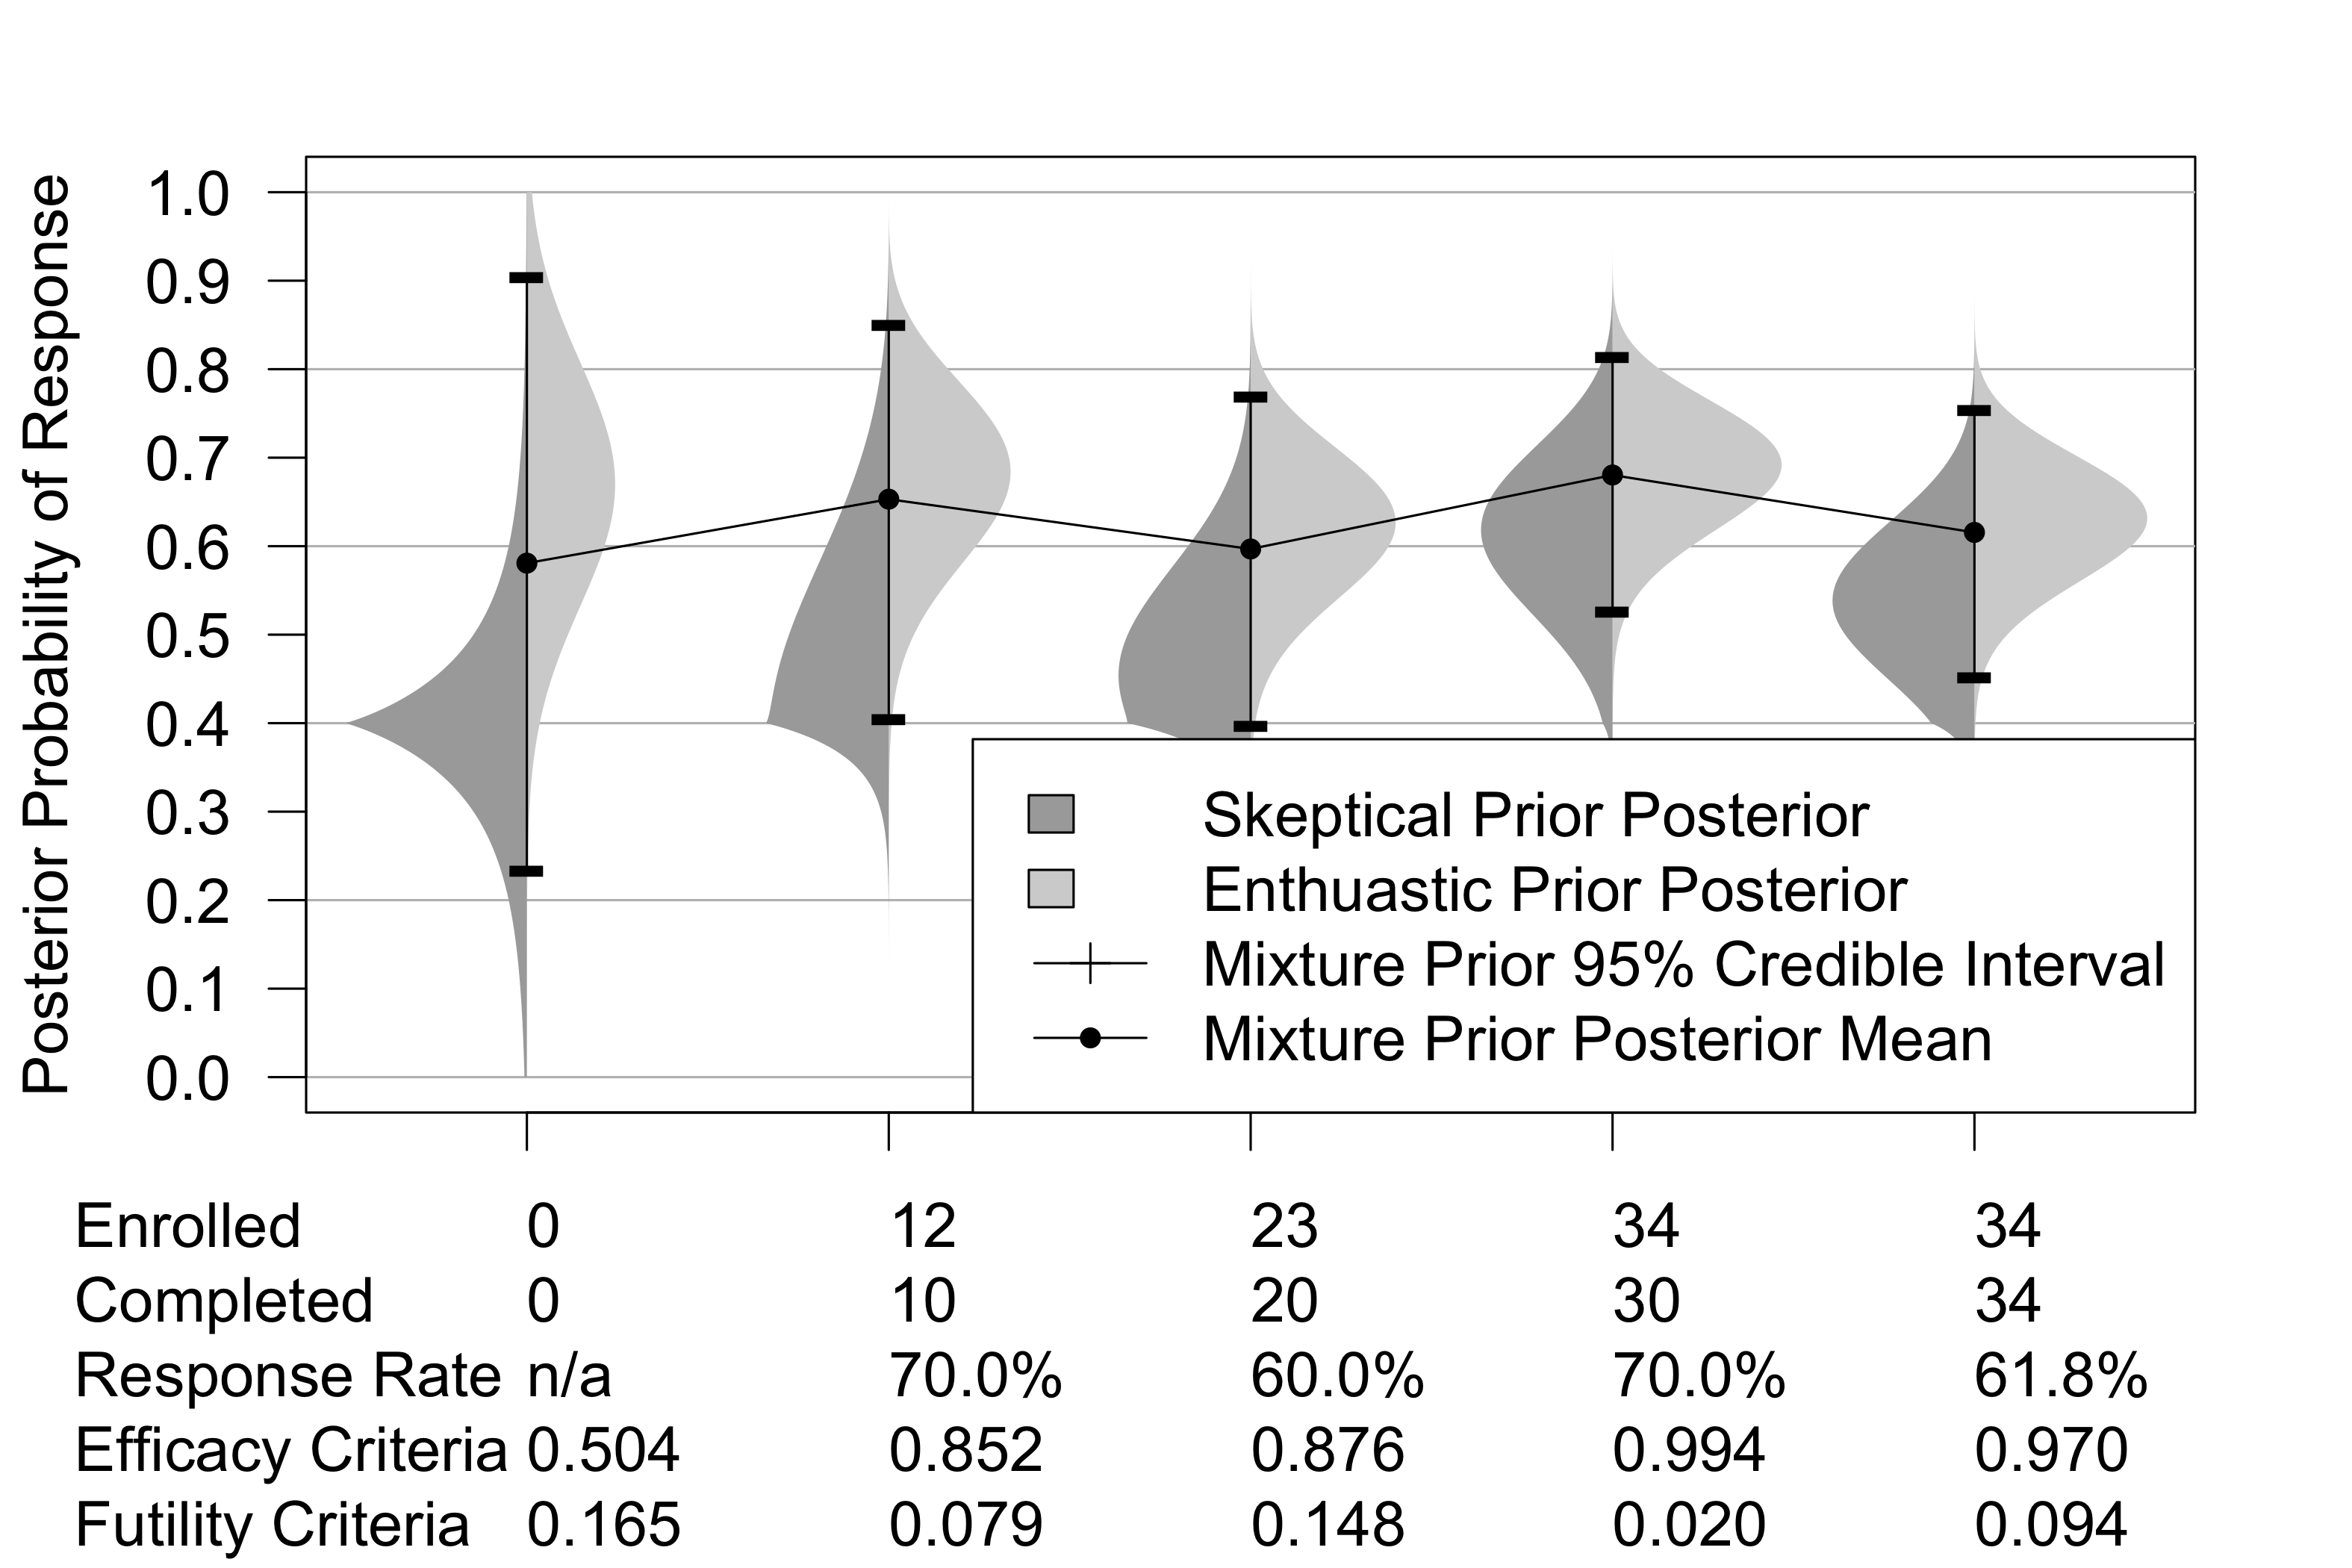
\includegraphics[width=7in]{./FIGURES/figure2a.png}
    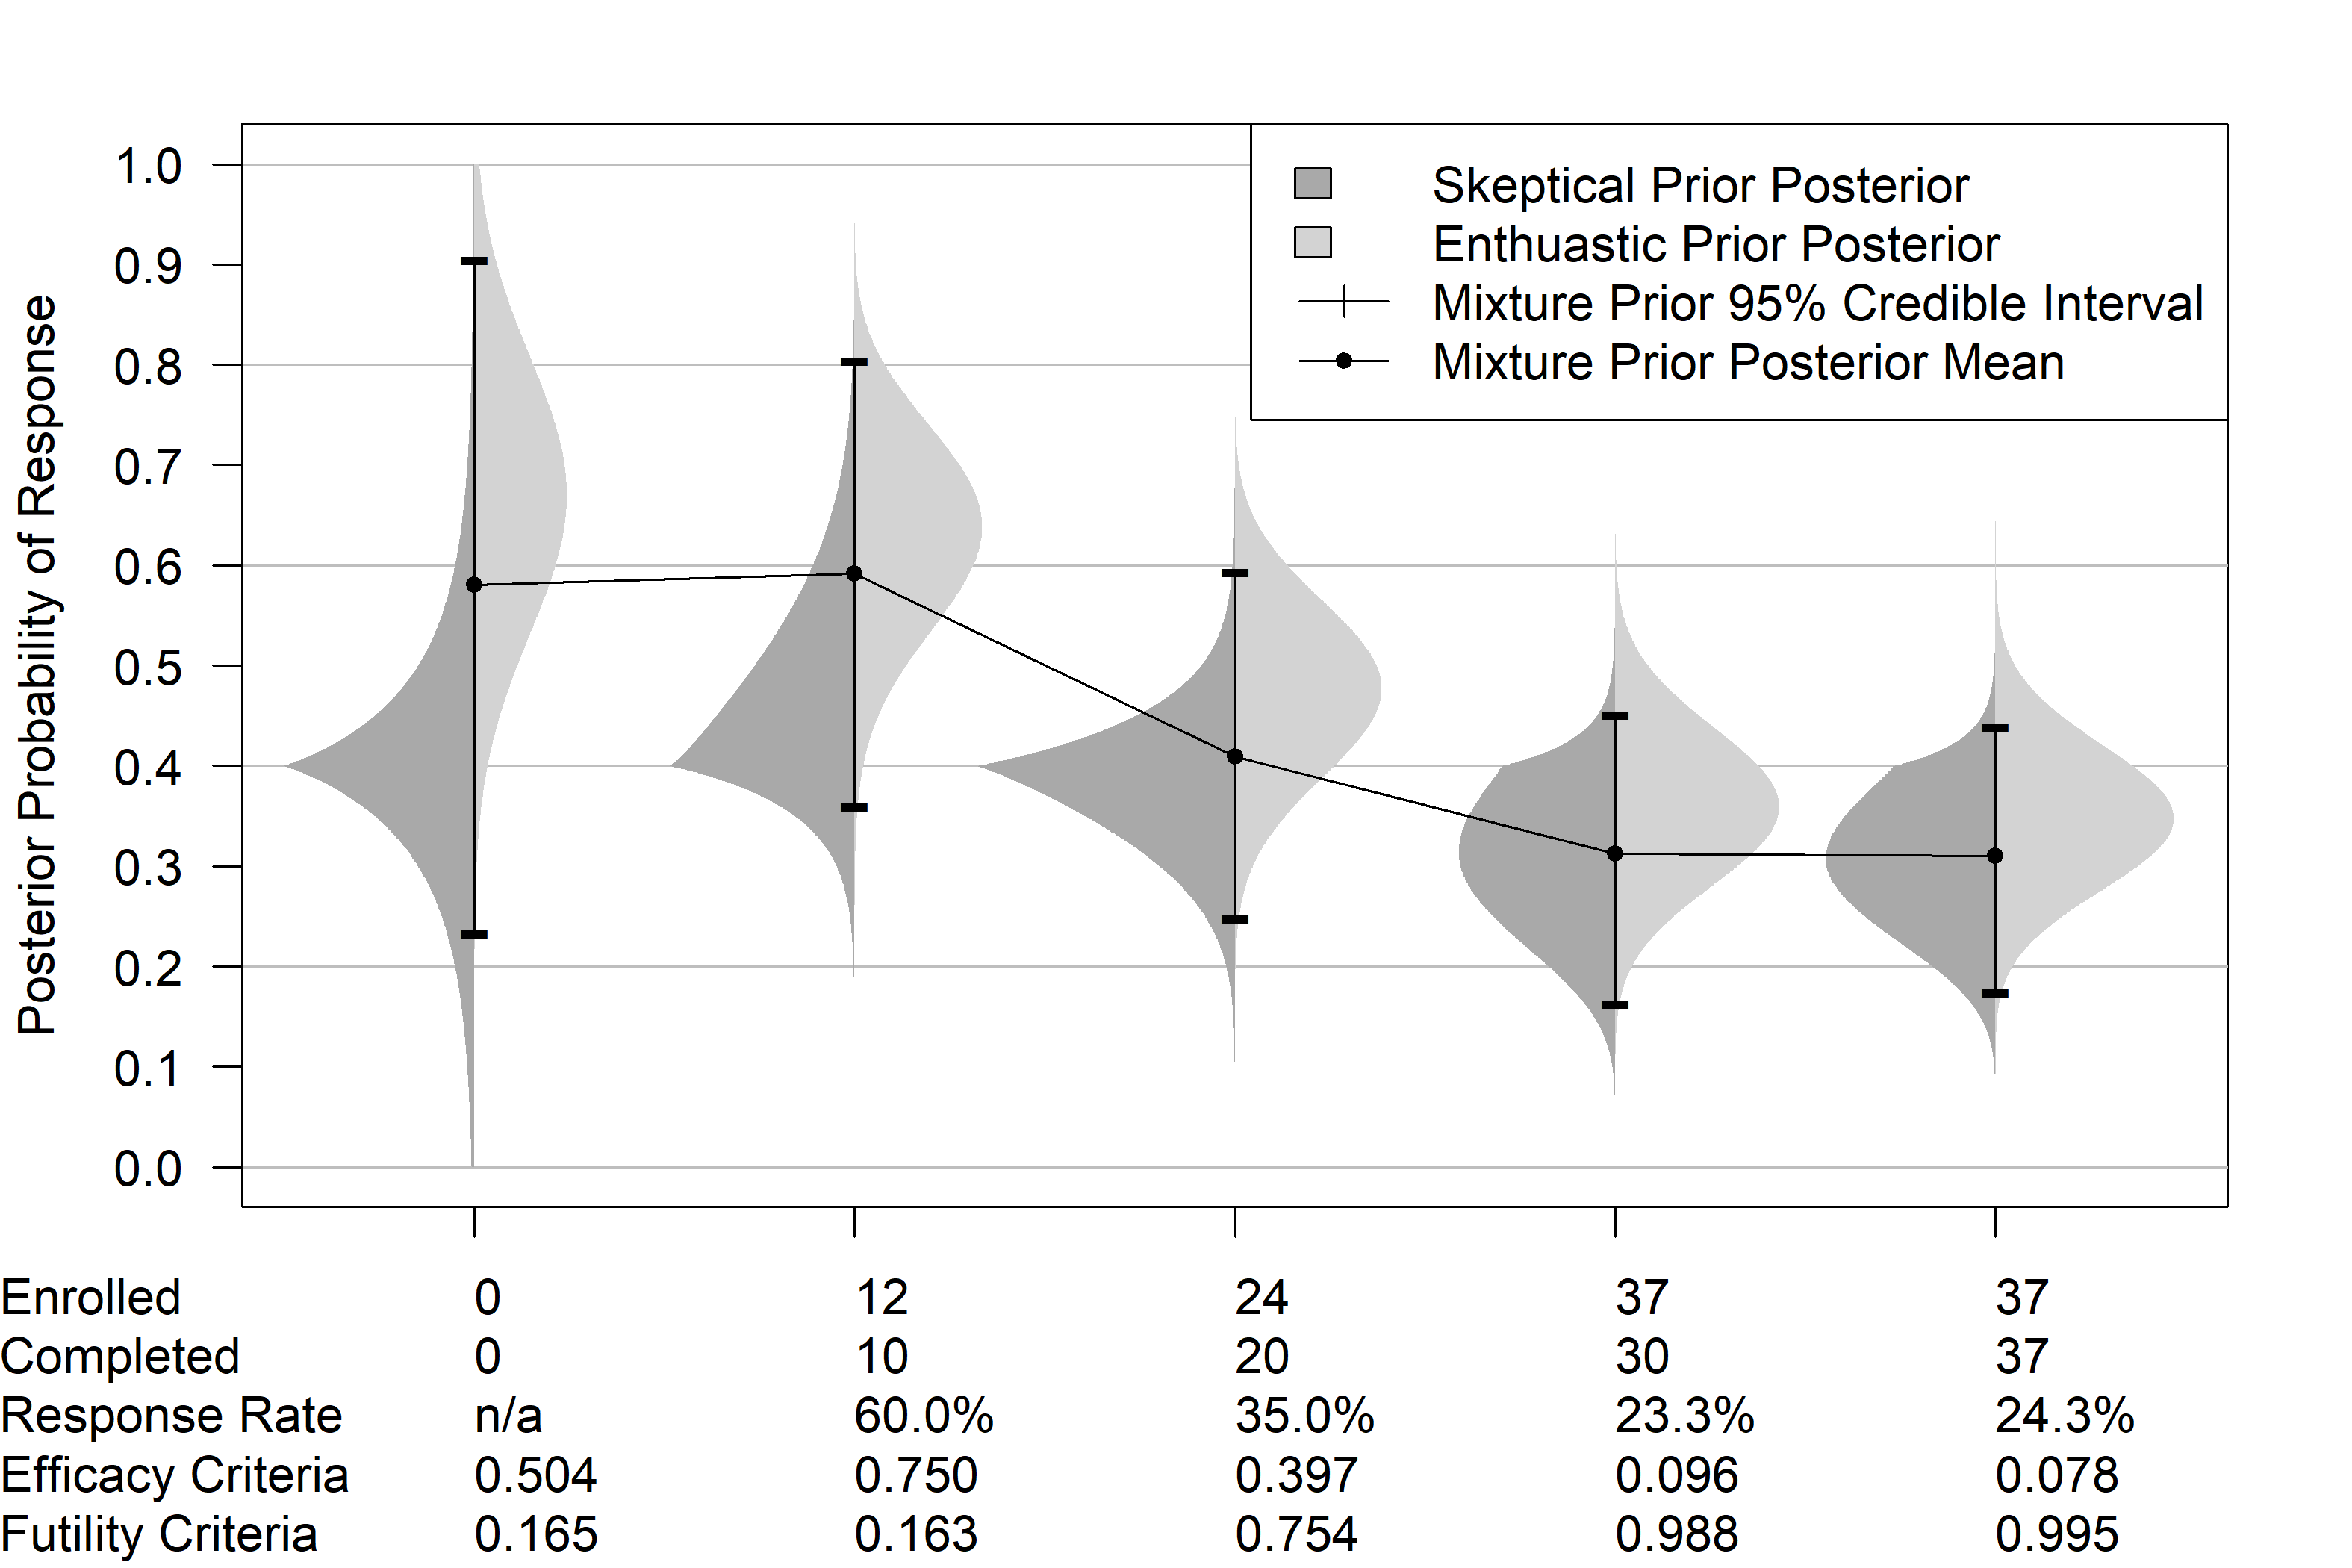
\includegraphics[width=7in]{./FIGURES/figure2b.png}
    \caption{A, Early stoppage for efficacy. B, early stoppage for futility.}
	\label{fig:figure2}

 
\end{center}\end{figure}
\subsubsection{Preposterior Analysis of Operating Characteristics}\label{sec:ex1.1}
An interim analysis will be completed after every 2 subjects complete follow-up. The inference prior is defined as the mixture \eqref{eq:inference_prior} with $\omega=0.5$ is used in evaluating the posterior mean and coverage probability.

Figure \ref{fig:ex1.1} shows the operating characters of this particular trial design. Stopping early for efficacy refers to satisfying \eqref{eq:ex1efficacy}, stopping early for futility refers to satisfying \eqref{eq:ex1futility}, and inconclusive findings refers to \eqref{eq:ex1maxss}. 

When the true response probability is $\theta=\theta_0$, there is a $3.9\%$ probability of stopping the trial early for efficacy. The posterior mean shows a slight bias towards the alternative hypothesis.

Figure \ref{fig:ex1.1} addresses the particular situation of when the efficacy criteria \eqref{eq:ex1efficacy} is satisfied at an interim analysis triggering termination of enrollment of additional subjects, but once the outcomes of subjects undergoing follow-up are ascertained the criteria is no longer satisfied. The distribution of the efficacy criteria given the final data for these cases are shown. The probability of these cases occurring is reflected by the percent agreement between interim and final results, and it is shown that as $\theta$ increases there is a higher probability of agreement and therefore a lower probability of evidence decrease.

The median efficacy criteria is very close to $1-\epsilon$ and in the vast majority of cases (greater than 10th percentile) the efficacy criteria is still very high. Therefore, for this trial design, the interim and final results are not highly discrepant with respect to the efficacy criteria in these cases.
\begin{figure}\begin{center}

    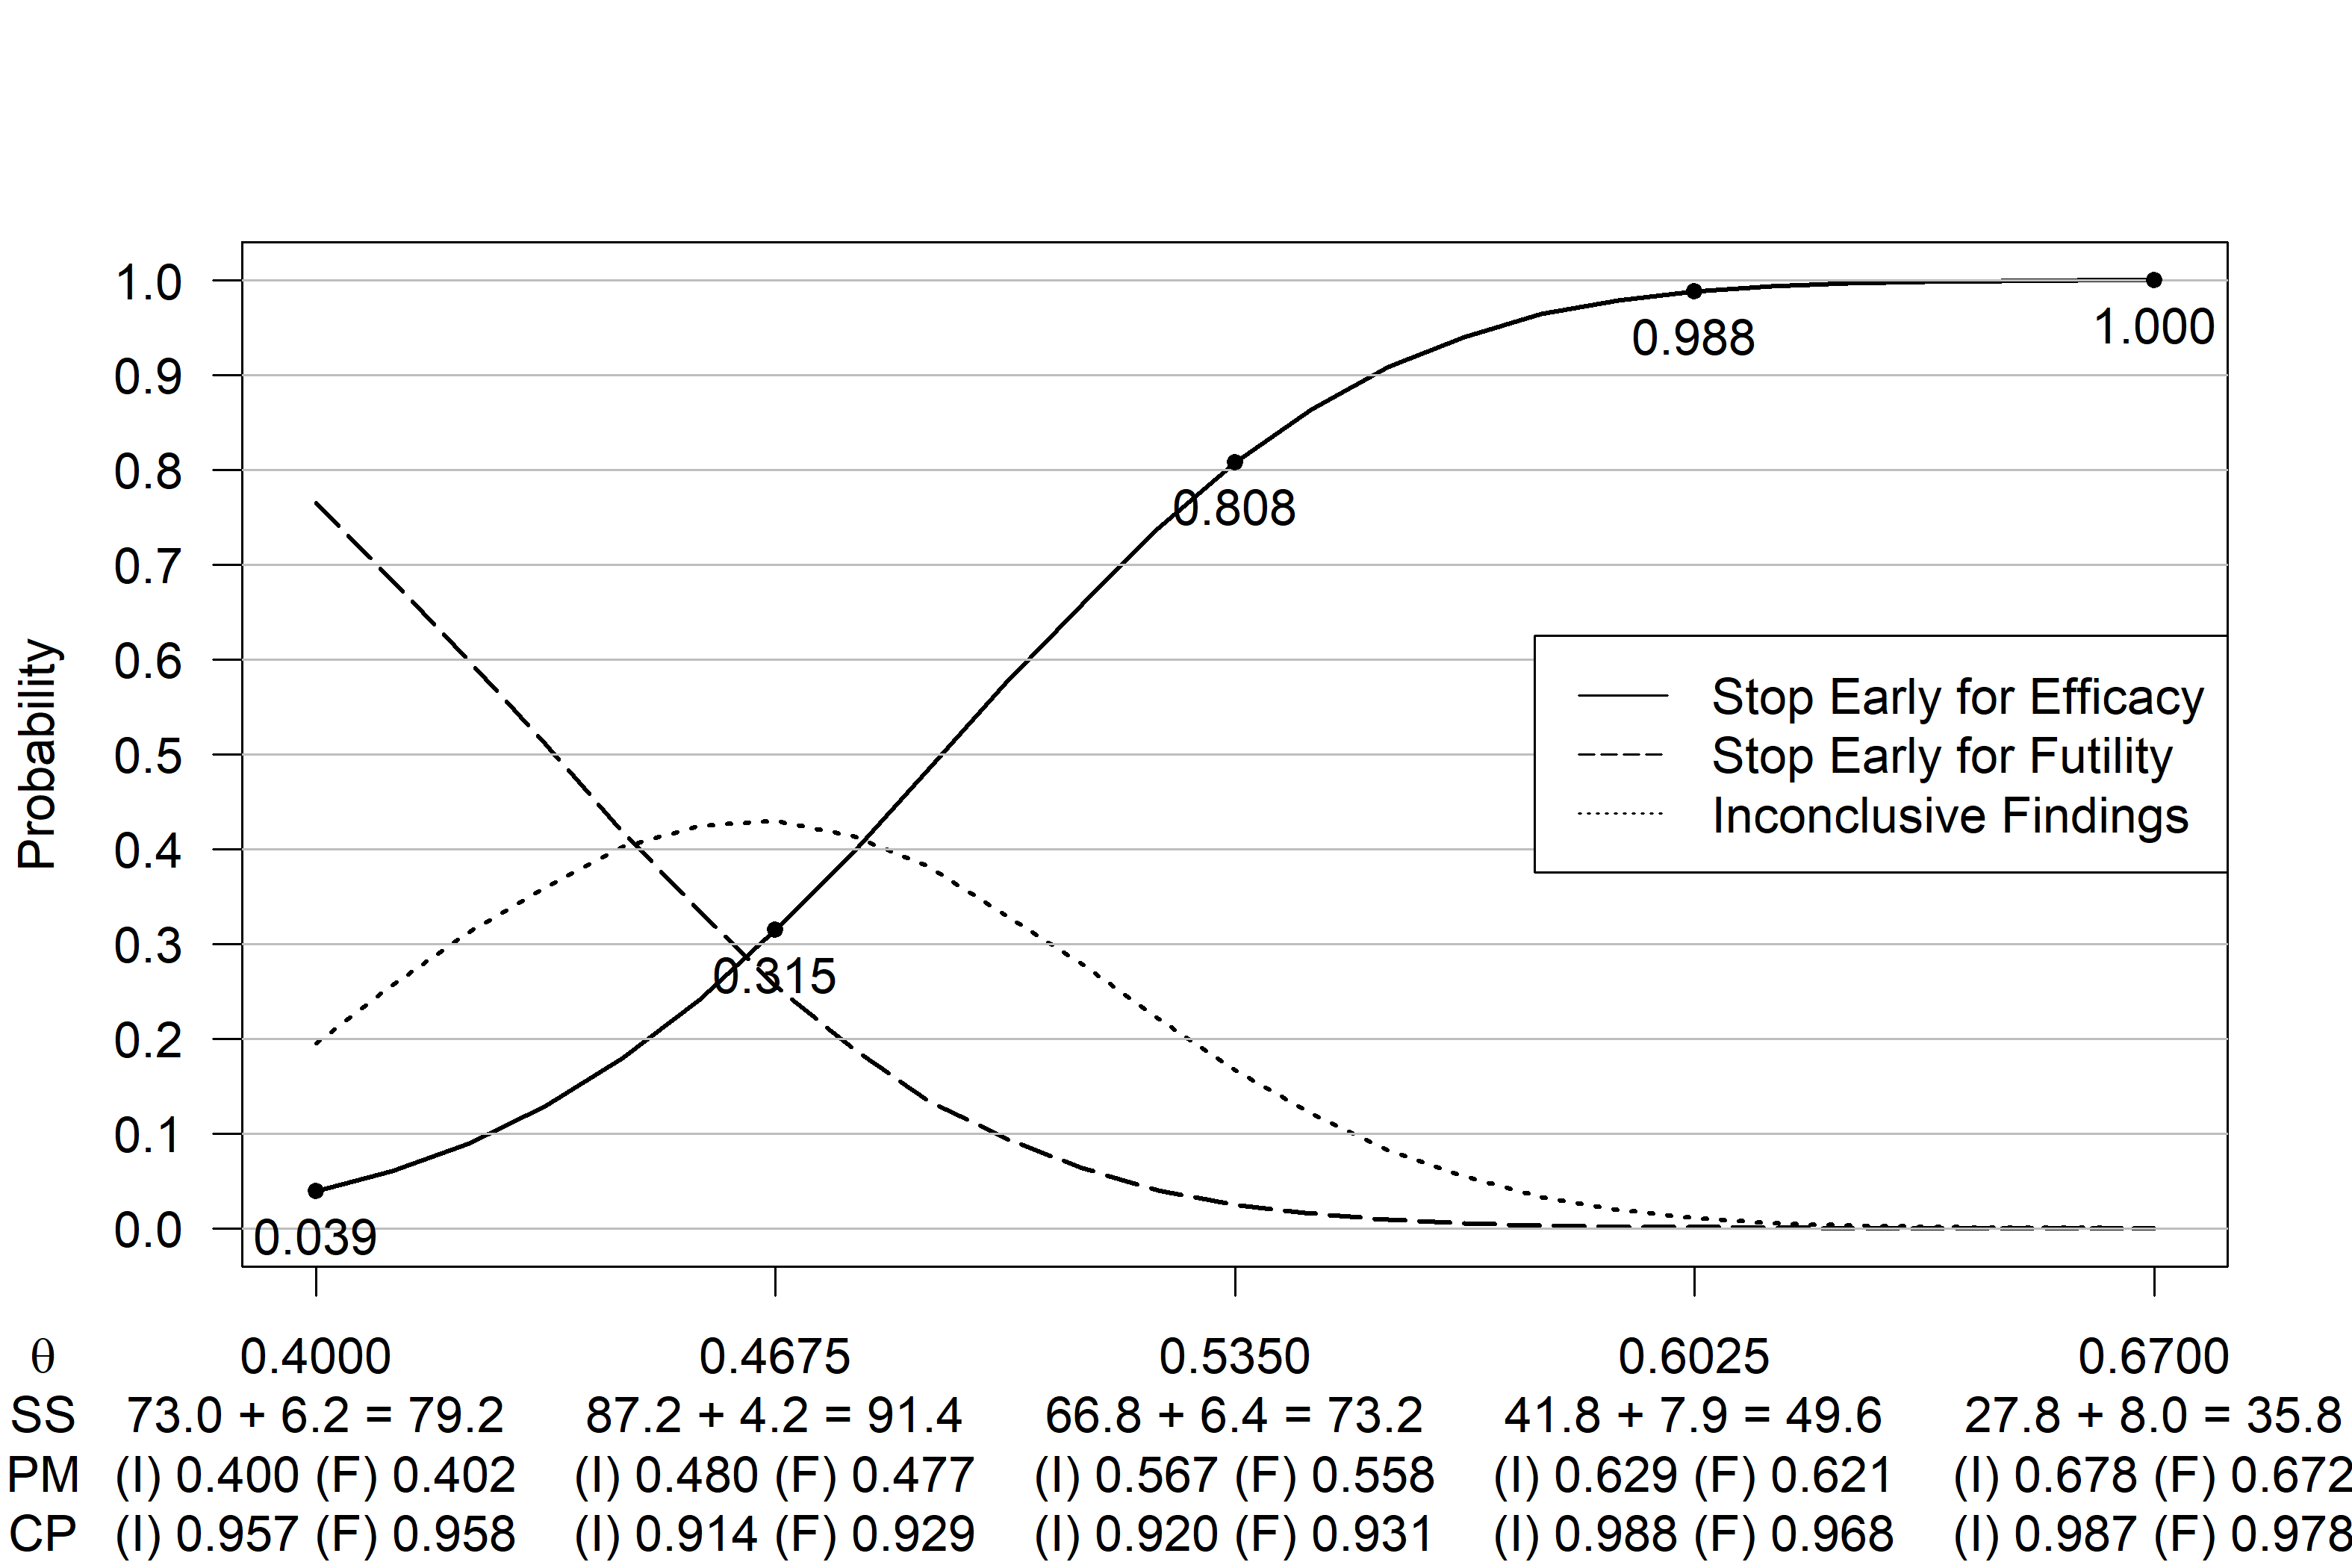
\includegraphics[width=6in]{./FIGURES/figure3a.png}
    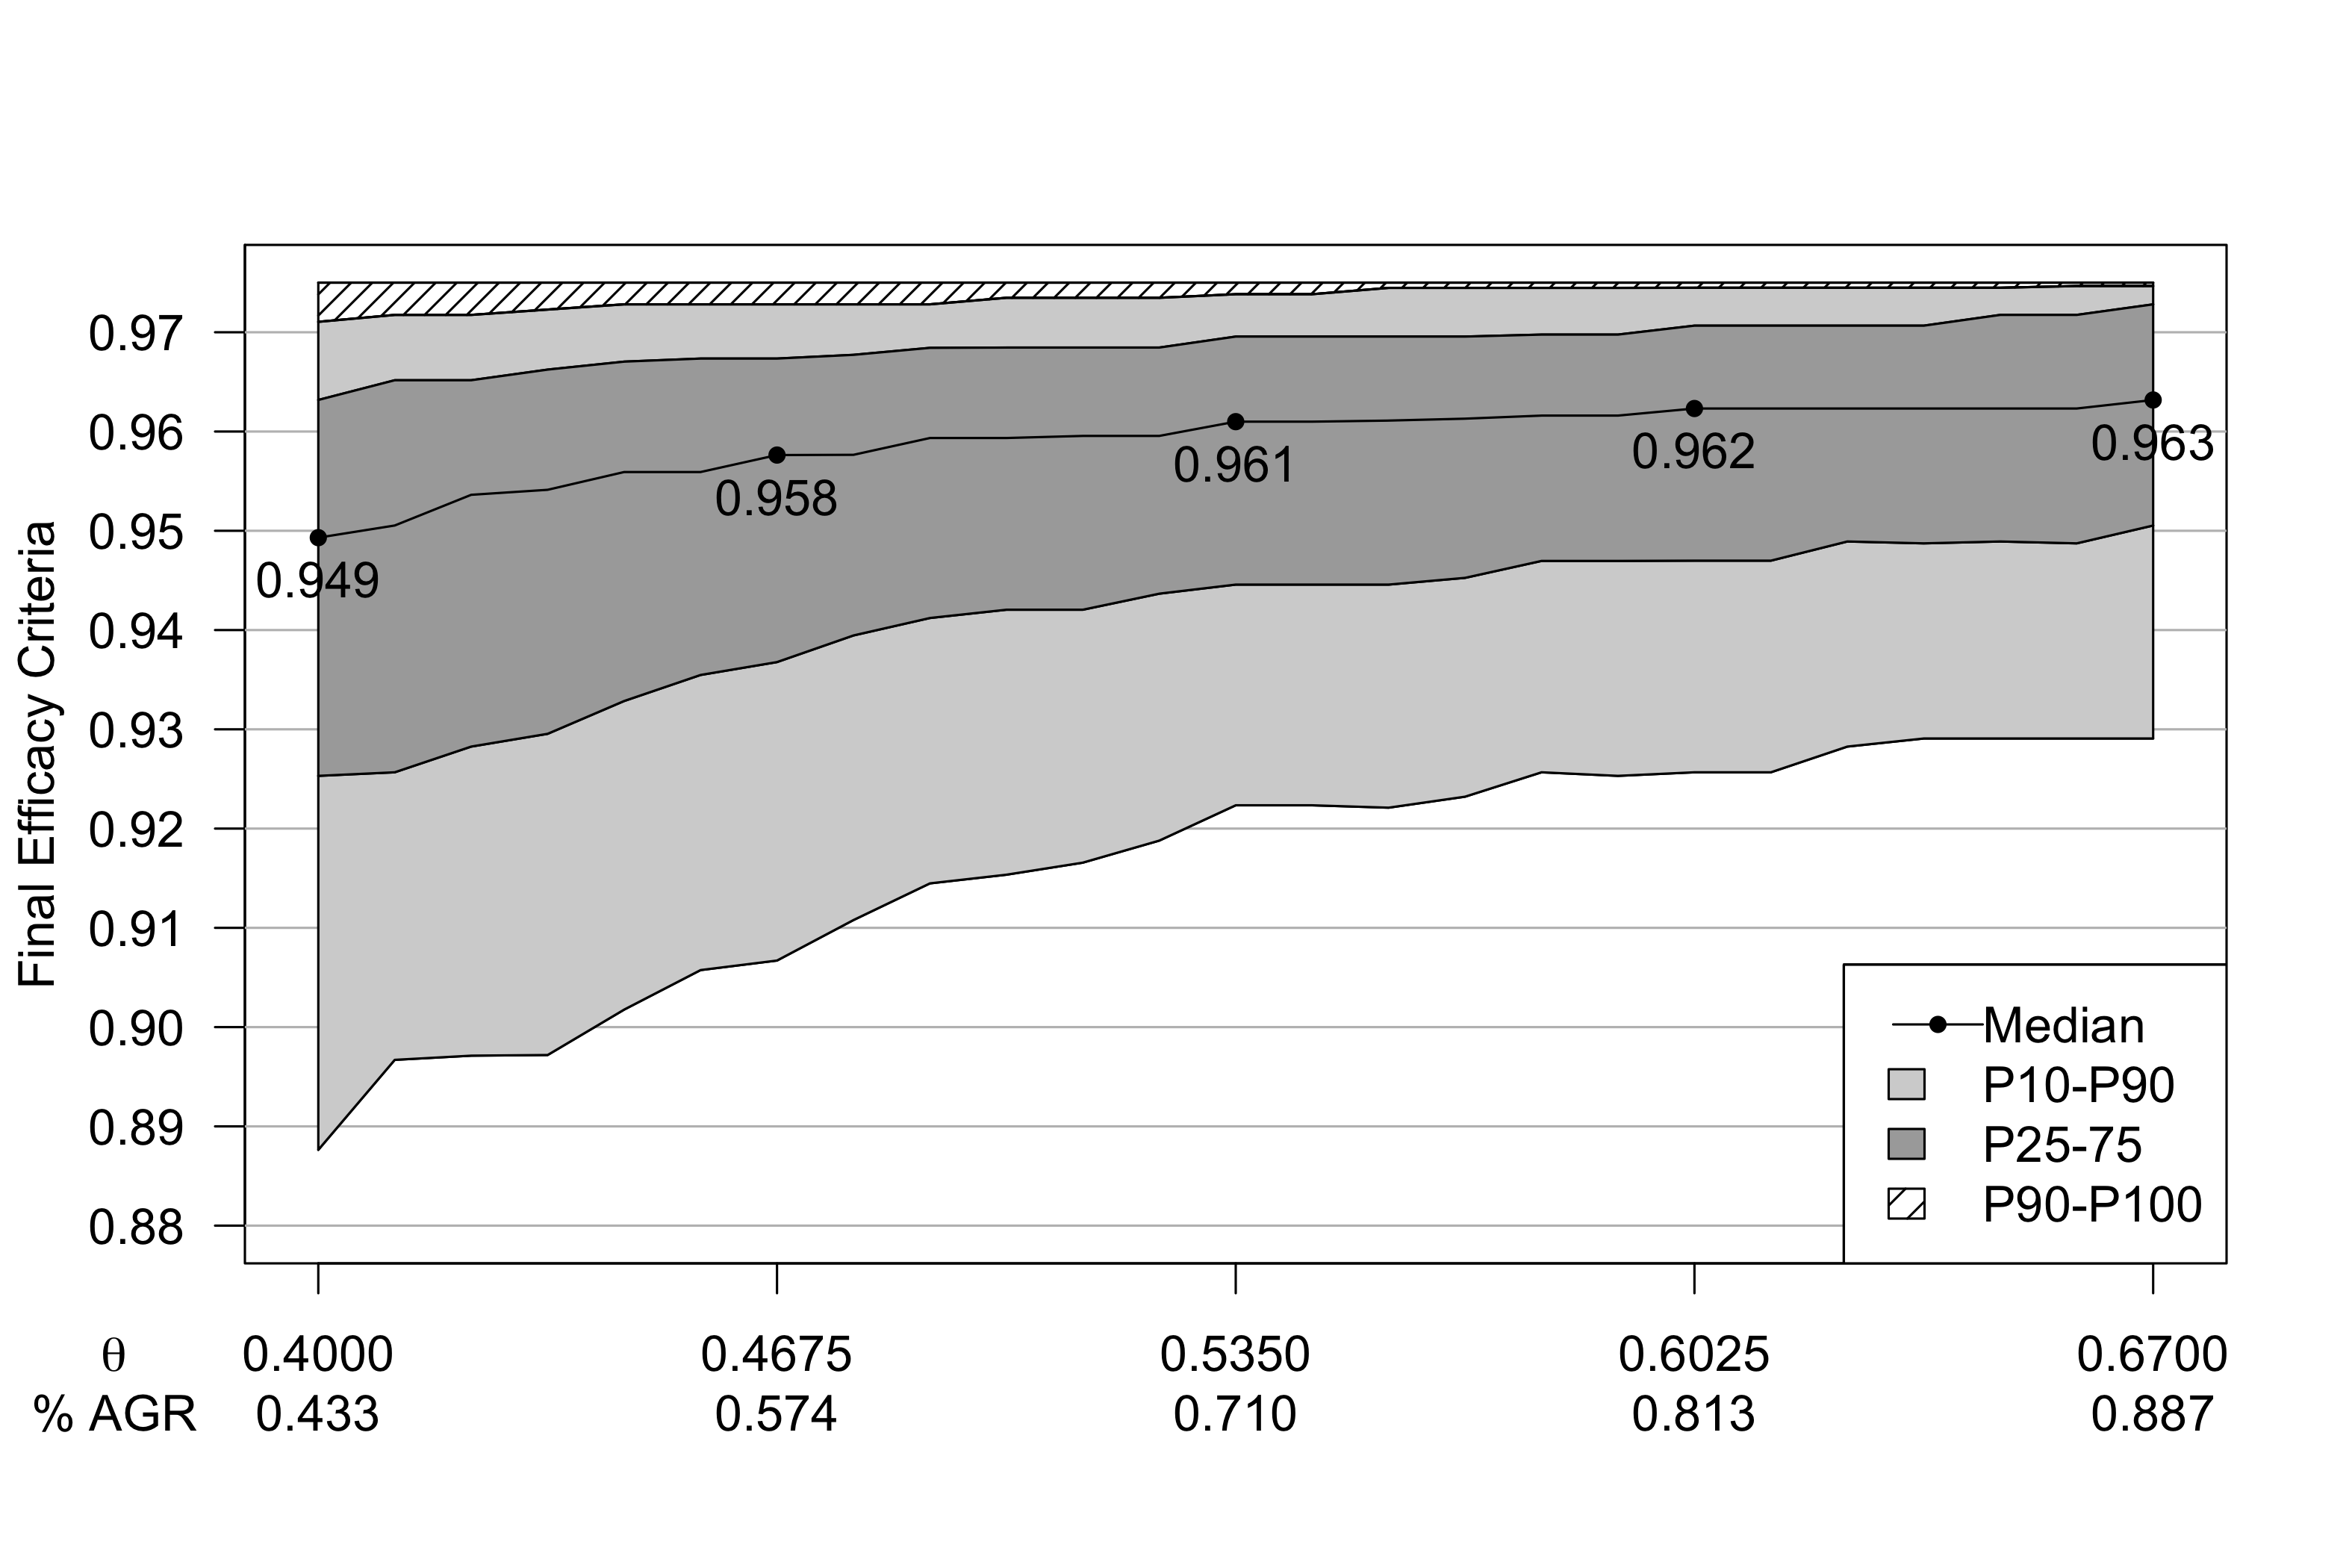
\includegraphics[width=6in]{./FIGURES/figure3b.png}
    \caption{A, Sequential design properties. (SS; sample size, PM; posterior mean, CP; coverage probability, (I); interim analysis, (F); final analysis) B, Distribution of final posterior probability given interim stoppage and evidence decrease ($\%$ AGR; Percent of agreement between final and interim posterior probabilities relative to $1-\epsilon$ threshold)}
	\label{fig:ex1.1}

\end{center}\end{figure}

%\subsubsection*{Vemurafenib Trial }
%``In this study, a response rate of 15\% at week
%8 was considered to be low, a response rate of
%45\% was considered to be high, and a response
%rate of 35\% was considered to be low but still
%desirable and indicative of efficacy. Assuming
%response rates as specified in the hypothesis testing, a power of 80\% for a high response rate and
%70\% for the low but still desirable response rate,
%and a two-sided alpha level of 0.1, we calculated
%that the number of patients required in each
%cohort would be 7, 13, or 19, depending on the
%results obtained."

\subsubsection{Type 1 error rate by the frequency of data monitoring}
Figure \ref{fig:ex1t1e} shows the probability of the efficacy criteria \eqref{eq:ex1efficacy} being satisfied at an interim or final analysis when $\theta=\theta_0$. The monitoring frequency is 1 when an interim analysis is made after every completed outcome (i.e. fully sequential), and is 112 (the maximum sample size) if the only analysis is done at the maximum sample size. 

The probability of the efficacy criteria being (errantly) satisfied is the highest for a fully sequential design, and decreases as the monitoring frequency decreases. However, the probability of the efficacy criteria being satisfied with the final data is very low for any type of sequential monitoring (under 0.02 in all cases).
\begin{figure}\begin{center}

    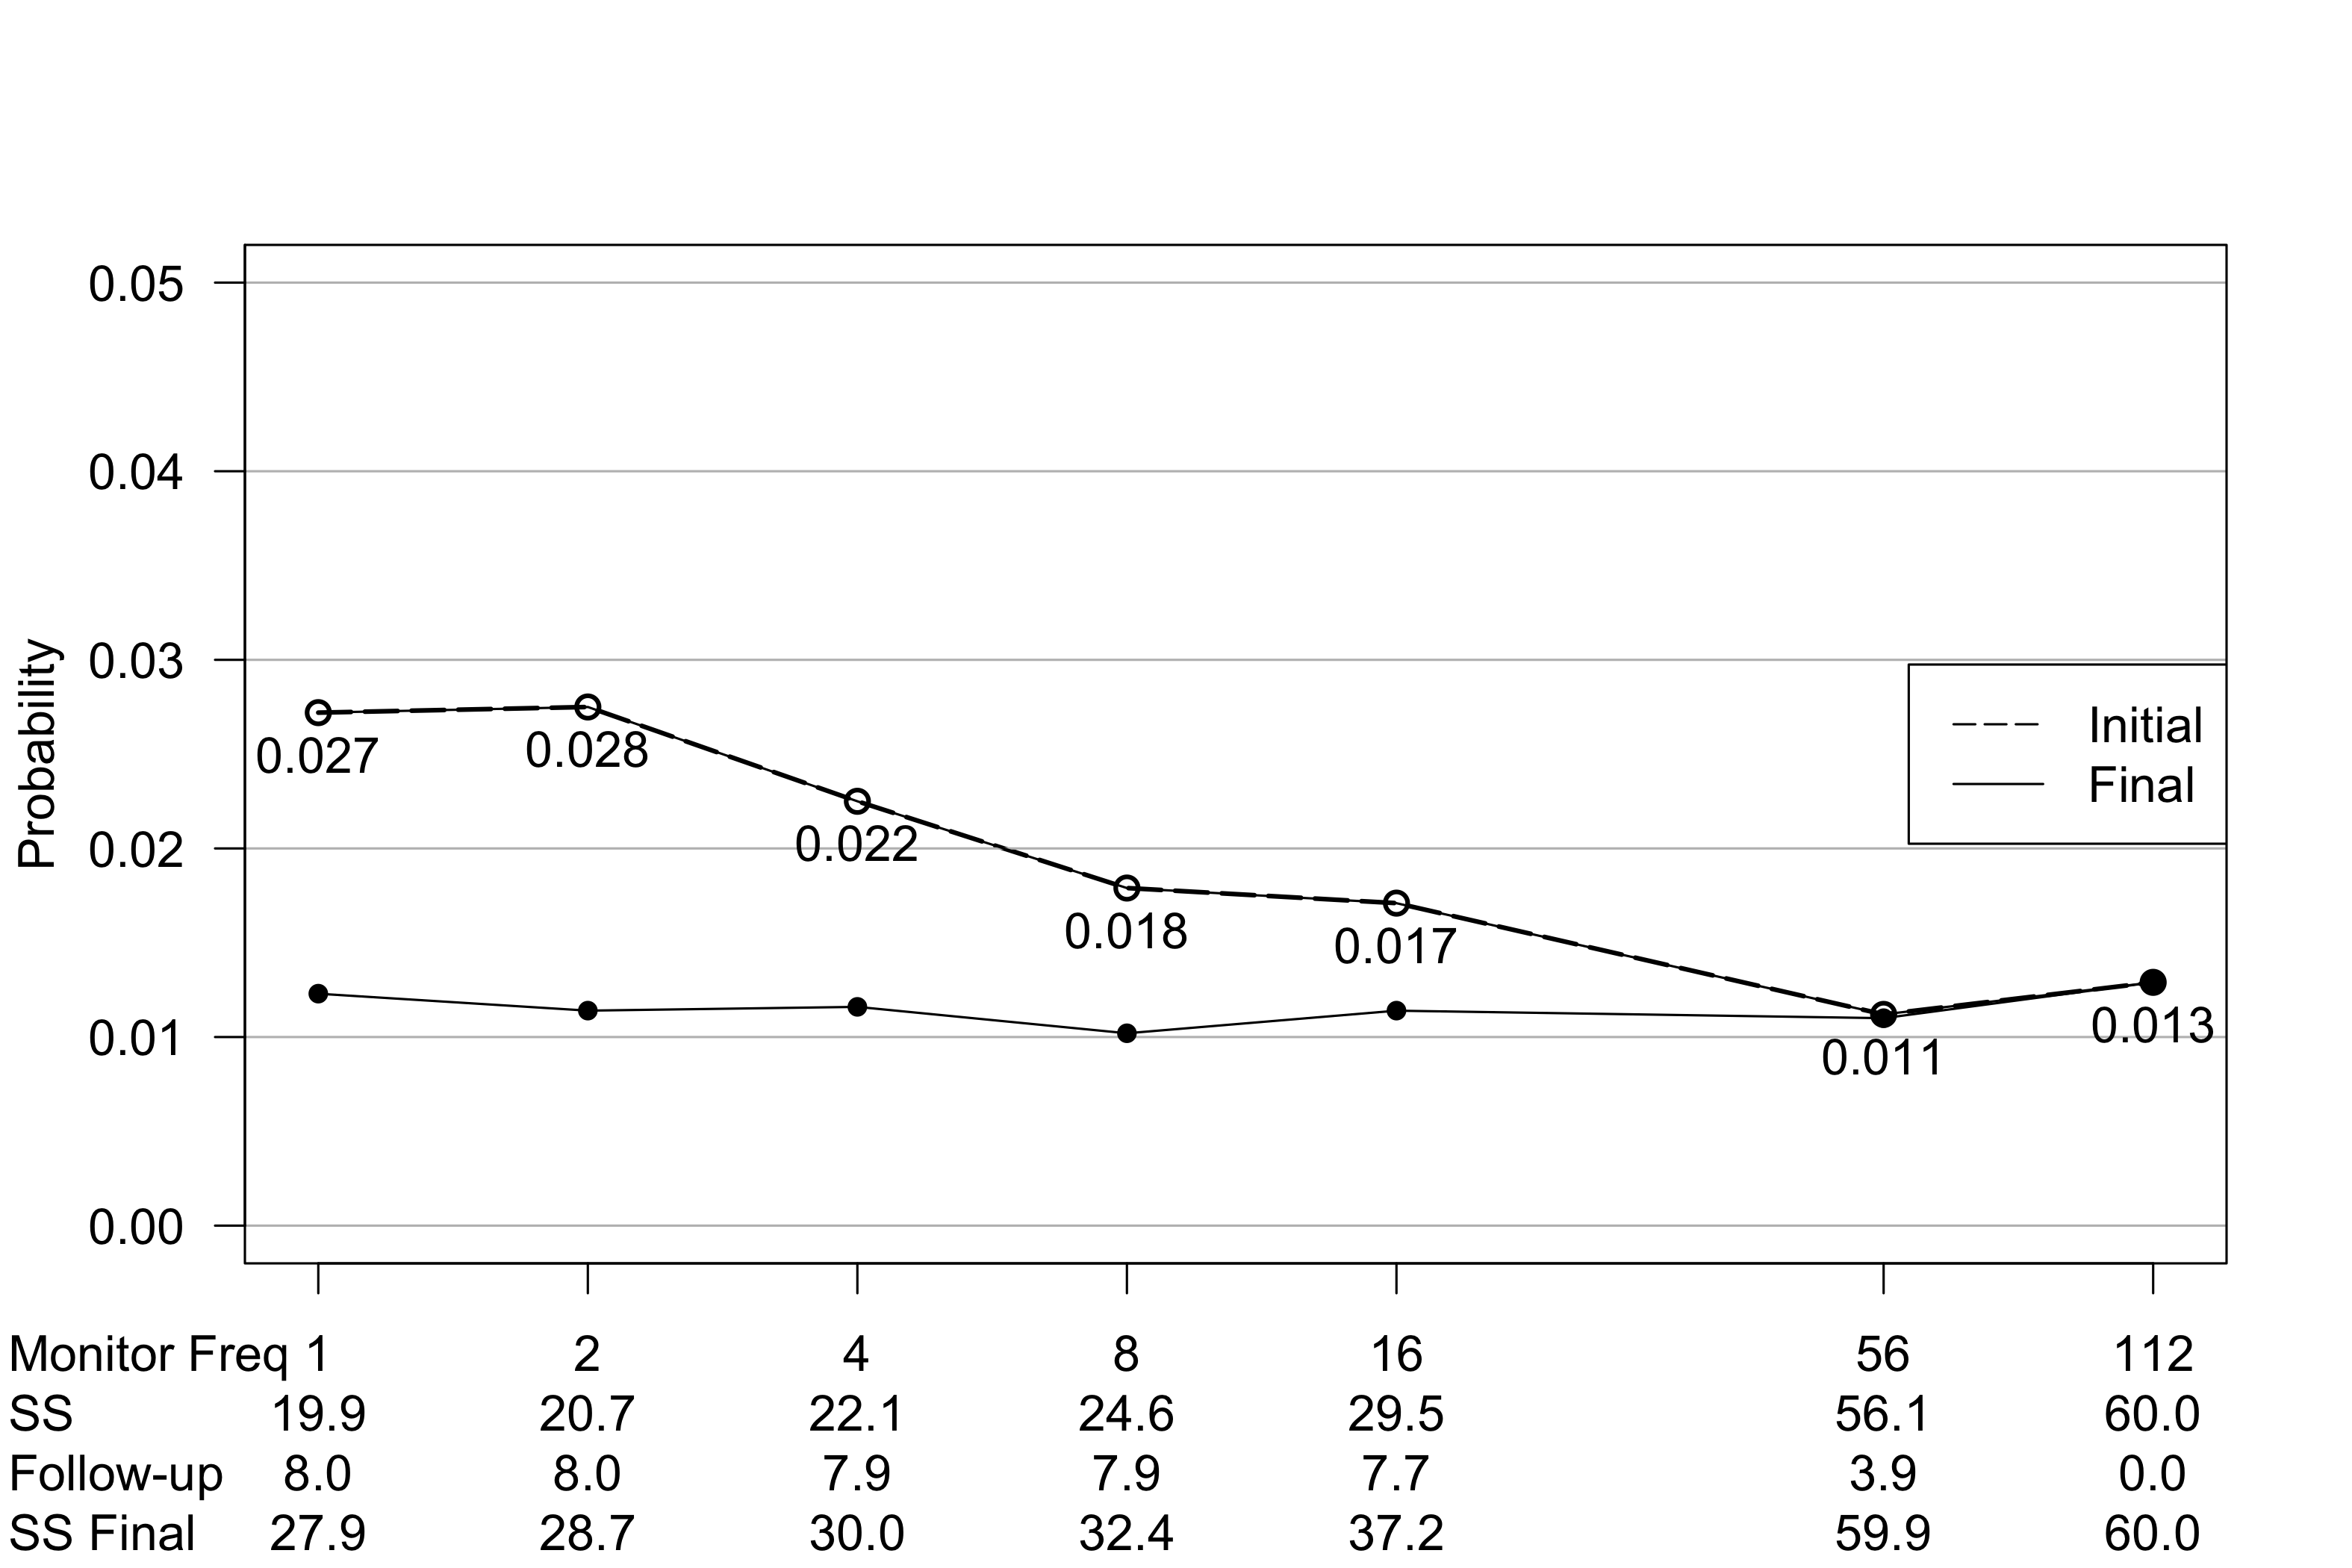
\includegraphics[width=6in]{./FIGURES/figure4.png}
    \caption{Probability of efficacy criteria being satisfied when $\theta=\theta_0$. SS; sample size. Monitor Freq; monitoring frequency.}
	\label{fig:ex1t1e}

%  \begin{subfigure}{7in}
%    \centering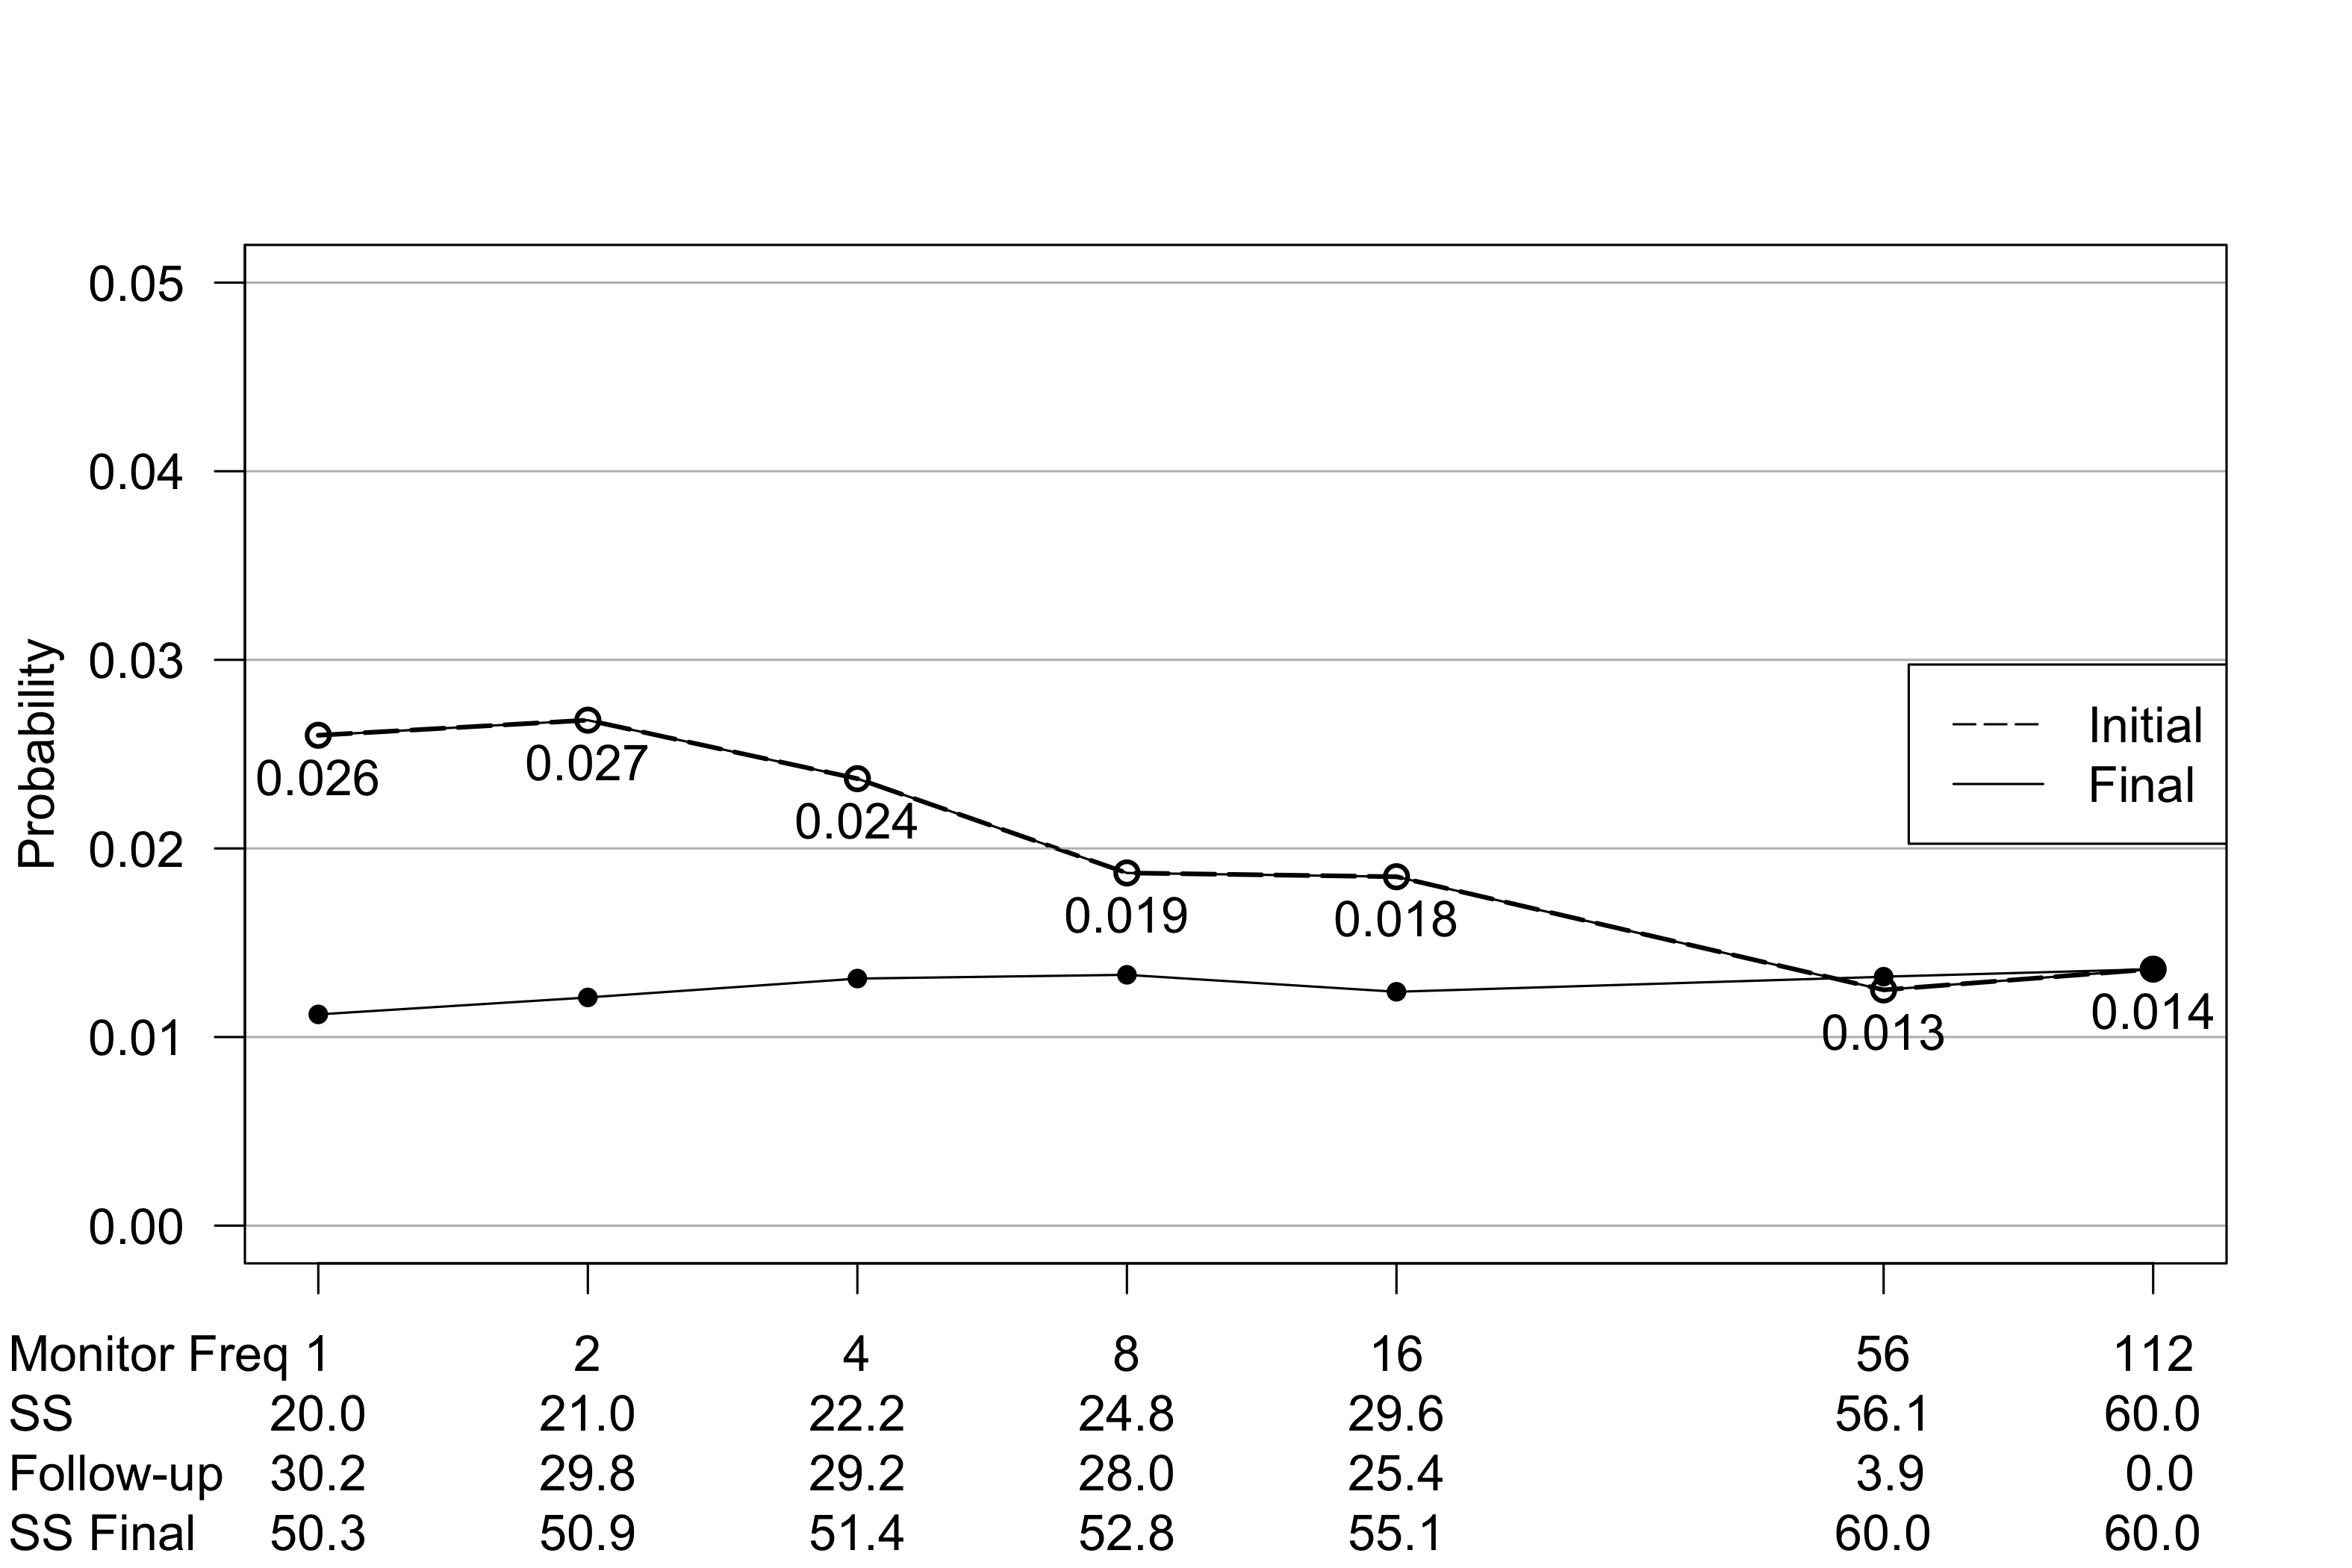
\includegraphics[width=7in]{./FIGURES/figureS1.png}
%    \caption{Caption text 2}
%  \end{subfigure}
 
\end{center}\end{figure}

%Even at the extreme case where an interim analysis is conducted after every outcome, the probability of stopping at the interim due to a promising result when the true response is at the null level is only $0.108$ (about double the nominal rate), and even in this situation the Type 1 error rate once follow-up is complete does not exceed $0.05$. Thus Bayesian sequential monitoring has good frequentist properties even with frequent interim analyses.
%\begin{itemize}
%\item The two sides of the discussion: first is what happens during the trial regarding sequential monitoring, such as \% of time stopping early vs. trial done to completion and expected sample size. Second is the final determination of efficacy or futility and how that relates to Type 1 Error and power. 
%\item  Remember the best case for sequential monitoring is slow enrollment relative to outcome ascertainment. Slow enrollment means there is a benefit to ending trial early and reach a conclusion faster. Outcome ascertainment needs to be somewhat fast to ensure a good \# of outcomes are generated.
%\end{itemize}
%\begin{itemize}
%\item Want to highlight that the ultimate inference will have no Type 1 error inflation. At this point the ultimate inference for efficacy is still made with skeptical prior.
%\item Label lines nicely.
%\item ``Only bad thing to do is to stop learning"
%\item Enrollment rate and \% of ongoing data as operating characteristics are interesting ideas, but focus on the plots already created.
%\item Mat: Scaling on \# of subjects in each interim analysis rather than \# of interim analyses (e.g. flip X axis). Make labels go vertical or diagonal.
%\end{itemize}

\subsection{Parallel Two-Group Design with Binary Endpoint}\label{sec:example2}
\subsubsection{Motivating example}
Consider the trial ``The Pediatric Lupus Trial of Belimumab Plus Background Standard Therapy (PLUTO)" (NCT01649765). Subjects were randomized to Belimumab 10mg/kg or placebo, and the primary endpoint was response at week 52. Response was measured by improvement in disease severity scores. The goal was to test for superiority of Belimumab to placebo. 

The study start date was September 7, 2012, and the primary completion date was January 24, 2018. Since the follow-up period is 52 weeks the last enrollment is estimated to be a year prior to the primary competition date yielding an average enrollment rate of one enrollment per $17.2$ days.

The study design included enrollment of 100 subjects, the first 24 subjects randomized in a 5:1 ratio (Belimumab:placebo) and the remaining 76 subjects would be randomized in a 1:1 allocation ratio. Therefore, 58 subjects would be randomized to Belimumab and 42 to placebo. The sample size was based on feasibility constraints rather than a power calculation, and the study was terminated after 93 subjects enrolled.

\subsubsection{Model formulation \& prior elicitation}\label{sec:example2model}
The data $\mathbf{D}$ are assumed to be independent Bernoulli random variables with response probability $\eta_0$ for the placebo group and $\eta_1$ for the treatment (IP for investigational product) group. The null response value for the difference $\theta_0=0$ and a highly efficacious difference is $\theta_1=0.12$. Consider the hypothesis testing of IP superiority to control $H_0:\theta\leq 0\text{ vs. }H_1: \theta>0$. An estimate for the treatment probability from adult trials is $\eta_1=0.51$.

%The location parameter is chosen to be $\mu=\theta_1-\delta_E=0.39$. The shape and scale parameters $\alpha$ and $\beta$ are chosen so that the prior is flat in the region $\mu\pm 0.10$ and is shown in Figure \ref{fig:figure5}(E). 

%The skeptical and enthusiastic priors are differentiated by their parameterizations for 
%\begin{align}
%\pi_S(\theta_1|\theta_0)\propto&\exp\left\{-\left(\frac{|\theta_1-\theta_0-\delta_0|}{\alpha_S}\right)^{\beta_S}\right\}\times f_S(\theta_0) \times I((\theta_0,\theta_1)\in [0,1]\times[0,1])\\
%\pi_E(\theta_1|\theta_0)\propto&\exp\left\{-\left(\frac{|\theta_1-\theta_0-\delta_1|}{\alpha_E}\right)^{\beta_E}\right\}\times f_E(\theta_0) \times I((\theta_0,\theta_1)\in [0,1]\times[0,1])
%\end{align}

%The values $\beta_S$ and $\beta_E$ are pre-specified and $\alpha_S$ and $\alpha_E$ are chosen to satisfy the tail-probability conditions.

%The complete skeptical and enthusiastic priors are then given by 
%\begin{align}
%\pi_S(\theta_0,\theta_1)\propto&\exp\left\{-\left(\frac{|\theta_0-\mu|}{\alpha}\right)^{\beta}\right\}\times \exp\left\{-\left(\frac{|\theta_1-\theta_0-\delta_0|}{\alpha_S}\right)^{\beta_S}\right\}\times I((\theta_0,\theta_1)\in [0,1]\times[0,1])\label{eq:ex2skpt}\\
%\pi_E(\theta_0,\theta_1)\propto&\exp\left\{-\left(\frac{|\theta_0-\mu|}{\alpha}\right)^{\beta}\right\}\times \exp\left\{-\left(\frac{|\theta_1-\theta_0-\delta_1|}{\alpha_E}\right)^{\beta_E}\right\}\times I((\theta_0,\theta_1)\in [0,1]\times[0,1])\label{eq:ex2enth}.
%\end{align}
%
%The joint priors $\pi_S(\theta_0,\theta_1)$ $\pi_E(\theta_0,\theta_1)$ as well as the marginal priors $\pi_S(\theta_1-\theta_0)$, $\pi_E(\theta_1-\theta_0)$ are shown in Figure \ref{fig:figure5}.
%
%where $c_S$ and $c_E$ are normalizing constants. The values of $\alpha_S$ and $\alpha_{S1}$ are chosen such that $P(\theta_1-\theta_0>0.1|\pi_S)=0.05$. Similarly, $\alpha_E$ and $\alpha_{E1}$ are chosen such that $P(\theta_1-\theta_0\leq0|\pi_E)=0.05$.

%\begin{align*}
%\pi(\theta_0,\theta_1)\propto& \hspace{0.05in}exp \left\{-\frac{1}{2}\left|\frac{(\theta_1-\theta_0)-\delta}{\alpha}\right|^\alpha\right\}
%\end{align*}


%Here we wish to elicit pessimistic and enthusiastic priors consistent with the following:
% \begin{enumerate}
%  \item The control group response probability is expected to be approximately $0.20$ and investigators are relatively sure
%		    that the it will be between 0.5 and 0.35.
%				
%	\item The IP group response probability is likely to provide an improvement of approximately 0.20.
%\end{enumerate}

Enrollment will proceed until one of the following three conditions are satisfied:
\begin{align*}
\text{Efficacy criteria (EFF): }&P(\theta>\delta_0|\mathbf{D},\pi_S)\geq 1-\epsilon %\label{eq:ex2efficacy}
\\
\text{Futility criteria (FUT): }&P\left(\theta \leq \frac{\delta_0+\delta_1}{2}\Big|\mathbf{D},\pi_E\right)\geq 1-\epsilon
%\label{eq:ex2futility}
\\
\text{Maximum sample size: }&N=100 \text{ patient outcomes}%\label{eq:ex2maxss}
\end{align*}

An interim analysis is competed after every 2 subjects have completed outcomes.

\subsubsection{Preposterior Analysis of Operating Characteristics}\label{sec:ex2operatingcharacteristics}
A mixture prior $\pi_I$ of the form \eqref{eq:inference_prior} is used for efficency monitoring where the choice of $\omega$ is chosen at the outset to be in the set $\{0.25,0.5,0.75,1\}$. Note that $\omega=1$ corresponds to the traditional skeptical prior and $\omega=0.5$ gives equal weight to the skeptical and enthusiastic components. When $\omega=0.25$ most of the weight to the enthusiastic component.

Figure \ref{fig:ex2varyomega} shows the probability of stopping early for efficacy (satisfying \eqref{eq:ex2efficacy}) based on the choice of $\omega$ used in the mixture prior for efficiency monitoring, and the associated sample sizes. Note that only in the case of $\omega=0.25$ is the probability of stopping the trial early for efficacy near 50\% when $\delta=\delta_1$. Also, only in the case of $\omega=0.25$ is the expected sample size less than 90. Therefore, for this design, the monitoring prior for efficacy has to be mostly enthusiastic in order for reasonable efficacy conditions.

\begin{figure}\begin{center}
    \centering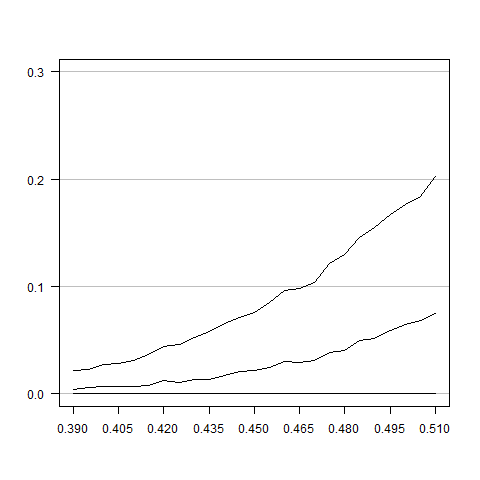
\includegraphics[width=7in]{./FIGURES/figure6.png}
    \caption{Probability of stopping for efficacy and associated sample sizes by choice of $\omega$ used in a mixture inference prior for efficacy monitoring.}
\label{fig:varyomega}
 \end{center}\end{figure}


\section{Discussion}

\section{Supplementary material}


\subsection{Type 1 error rate depending on enrollment schemes}
Recall Figure \ref{fig:ex1t1e} from Section \ref{sec:example1} which showed Type 1 error properties for the single-arm design. Figure \ref{fig:ex1t1e_longer} shows results from a design that has a longer follow-up period. The interim sample sizes are the same for each monitoring frequency, however, the final sample sizes under the longer follow-up designs are much larger (over 20 subjects in follow-up for monitoring frequencies of 8 or fewer, compared to approximately 6 subjects in the shorter follow-up designs). The final probability of efficacy criteria being satisfied is generally slightly lower in the longer follow-up design, which is what we would expect since the larger final sample size contains more data consistent with a null result.
\begin{figure}\begin{center}

   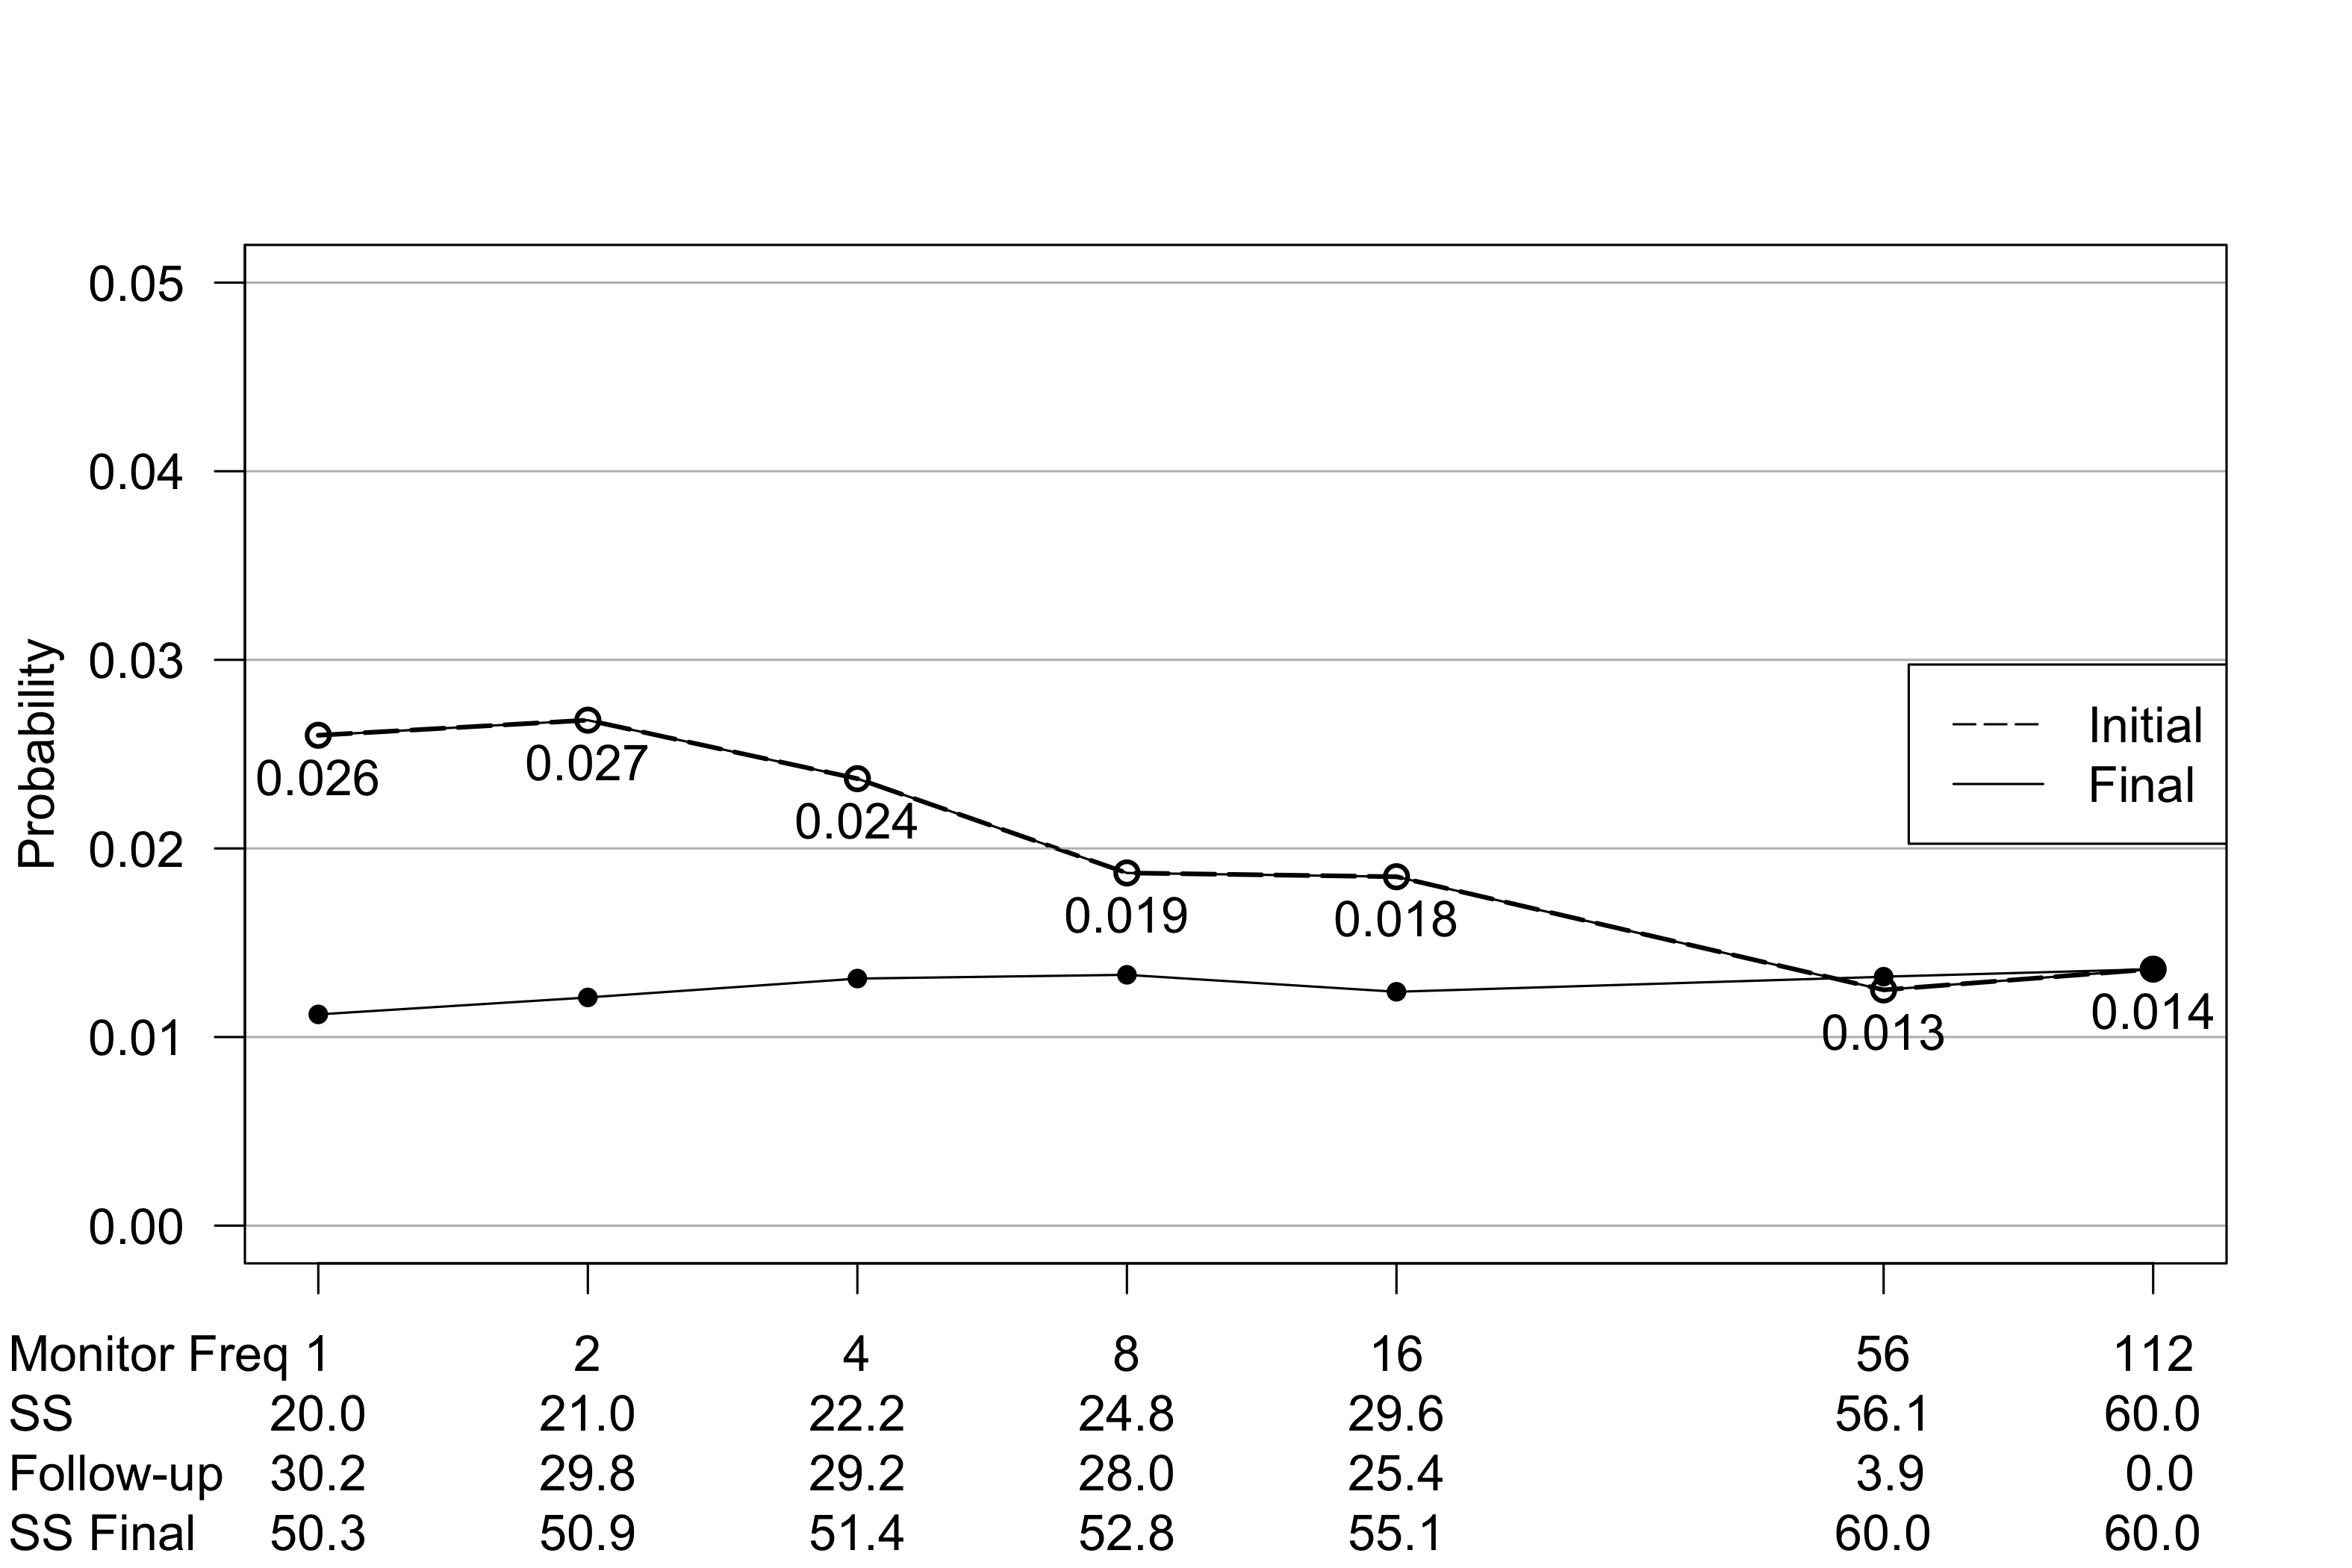
\includegraphics[width=6in]{./FIGURES/figureS1.png}
    \caption{Single arm design from Example \ref{sec:example1} with a longer follow-up period. Probability of efficacy criteria being satisfied when $\theta=\theta_0$. SS; sample size. Monitor Freq; monitoring frequency.}
	\label{fig:ex1t1e_longer}

\end{center}\end{figure}


\subsection{Robustness of parameterizations of monitoring priors}\label{sec:priorRobustness}
The analyses done in Section \ref{sec:example1} used a concentrate skeptical prior and default enthusiastic prior. In this section we show the four possible designs using the combinations of skeptical and enthusiastic prior given in Figure \ref{fig:figure1}.

Figures \ref{fig:robustness1}-\ref{fig:robustness2} shows what happens when the enthusiastic prior shifts from default to flattened, with the skeptical prior remaining fixed. Note that in the region between $\theta_0$ and $\frac{\theta_0+\theta_1}{2}$ as the enthusiastic prior shifts from default to flattened, (a) the probability of stopping early for futility increases (b) the probability of inconclusive findings decreases and (c) the intermediate and final sample sizes decrease. This is because the enthusiastic prior gives more mass in for this region of $\theta$. The flattened enthusiastic prior was used in Section \ref{sec:example1} to enhance the ability of futility monitoring to reduce the sample size.

Contrasting \ref{fig:robustness1} and \ref{fig:robustness2}, we see that the probability of stopping early for efficacy is much higher at $\theta_0$ when the default skeptical prior is used rather than the concentrated skeptical prior. This is because the default skeptical prior has less mass around $\theta=\theta_0$, therefore it is easier to convince the skeptic that $\theta>\theta_0$ under the null result $\theta=\theta_0$. The concentrated skeptical prior was used in Section \ref{sec:example1} to limit this probability and provide better Type 1 error control.

The choice of skeptical and enthusiastic prior affects the analysis, and their specification (e.g. default, skeptical, enthusiastic) should be made with these properties in mind.

\begin{figure}\begin{center}

 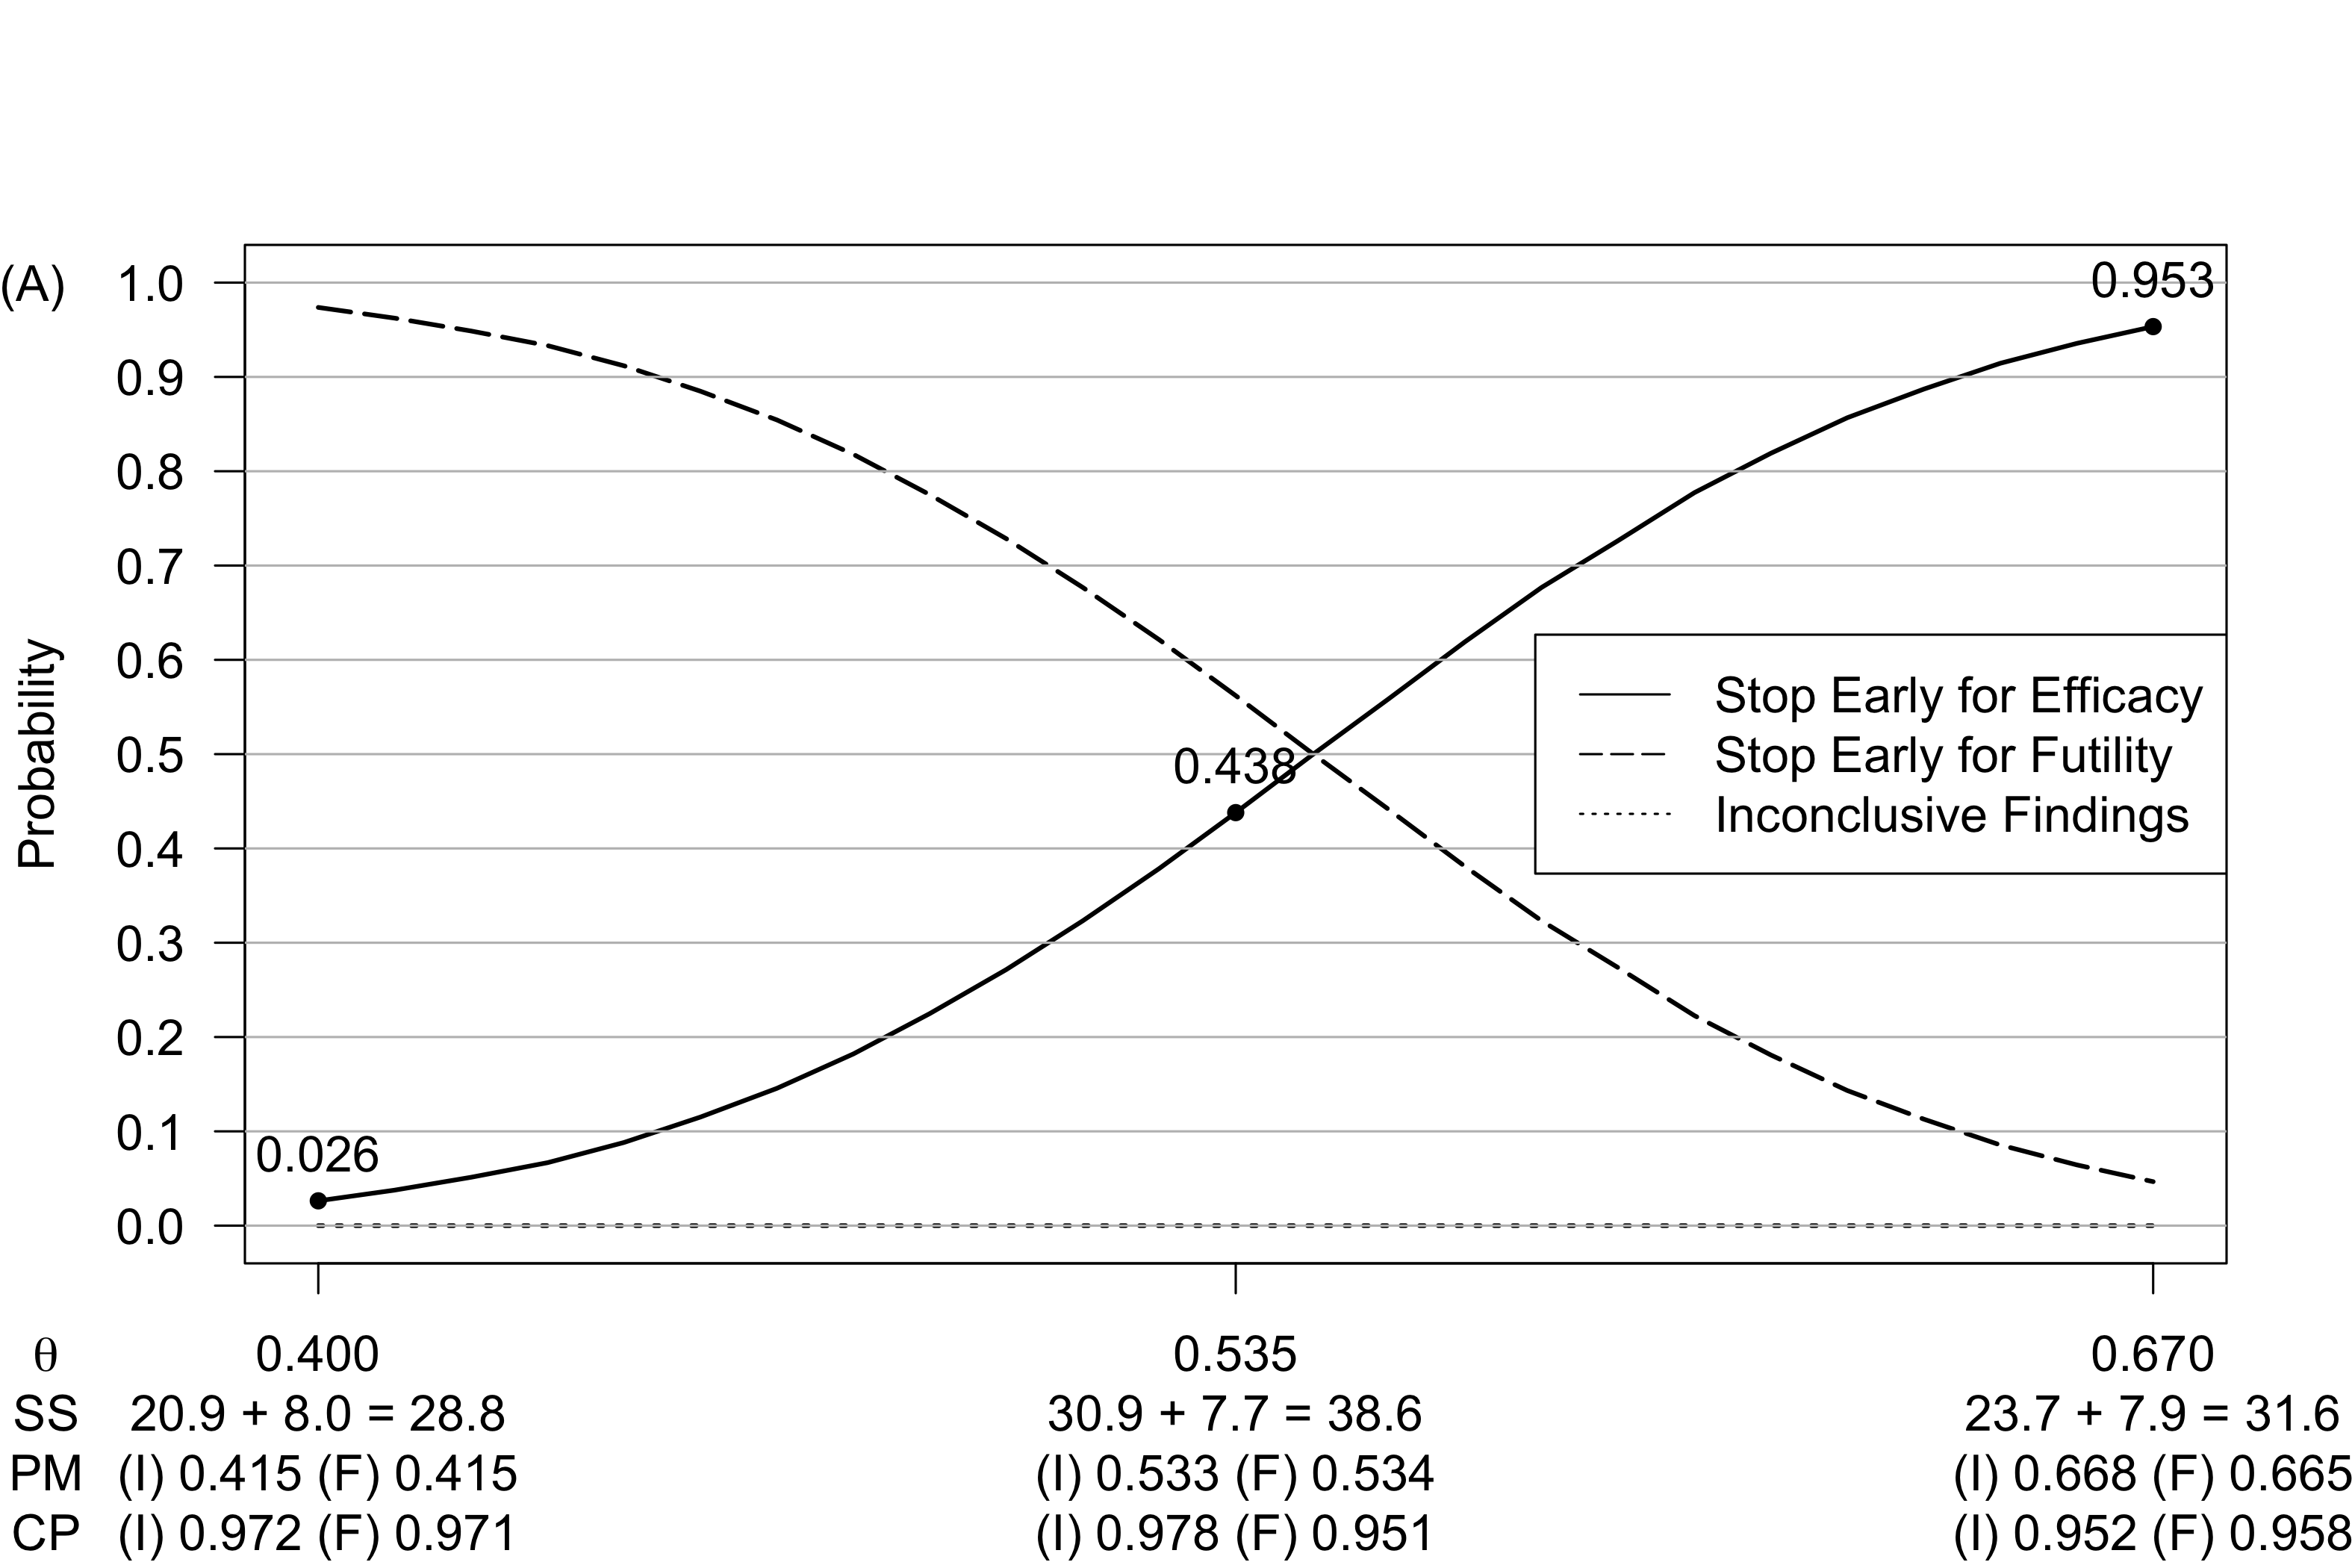
\includegraphics[width=7in]{./FIGURES/figureS2a.png}
 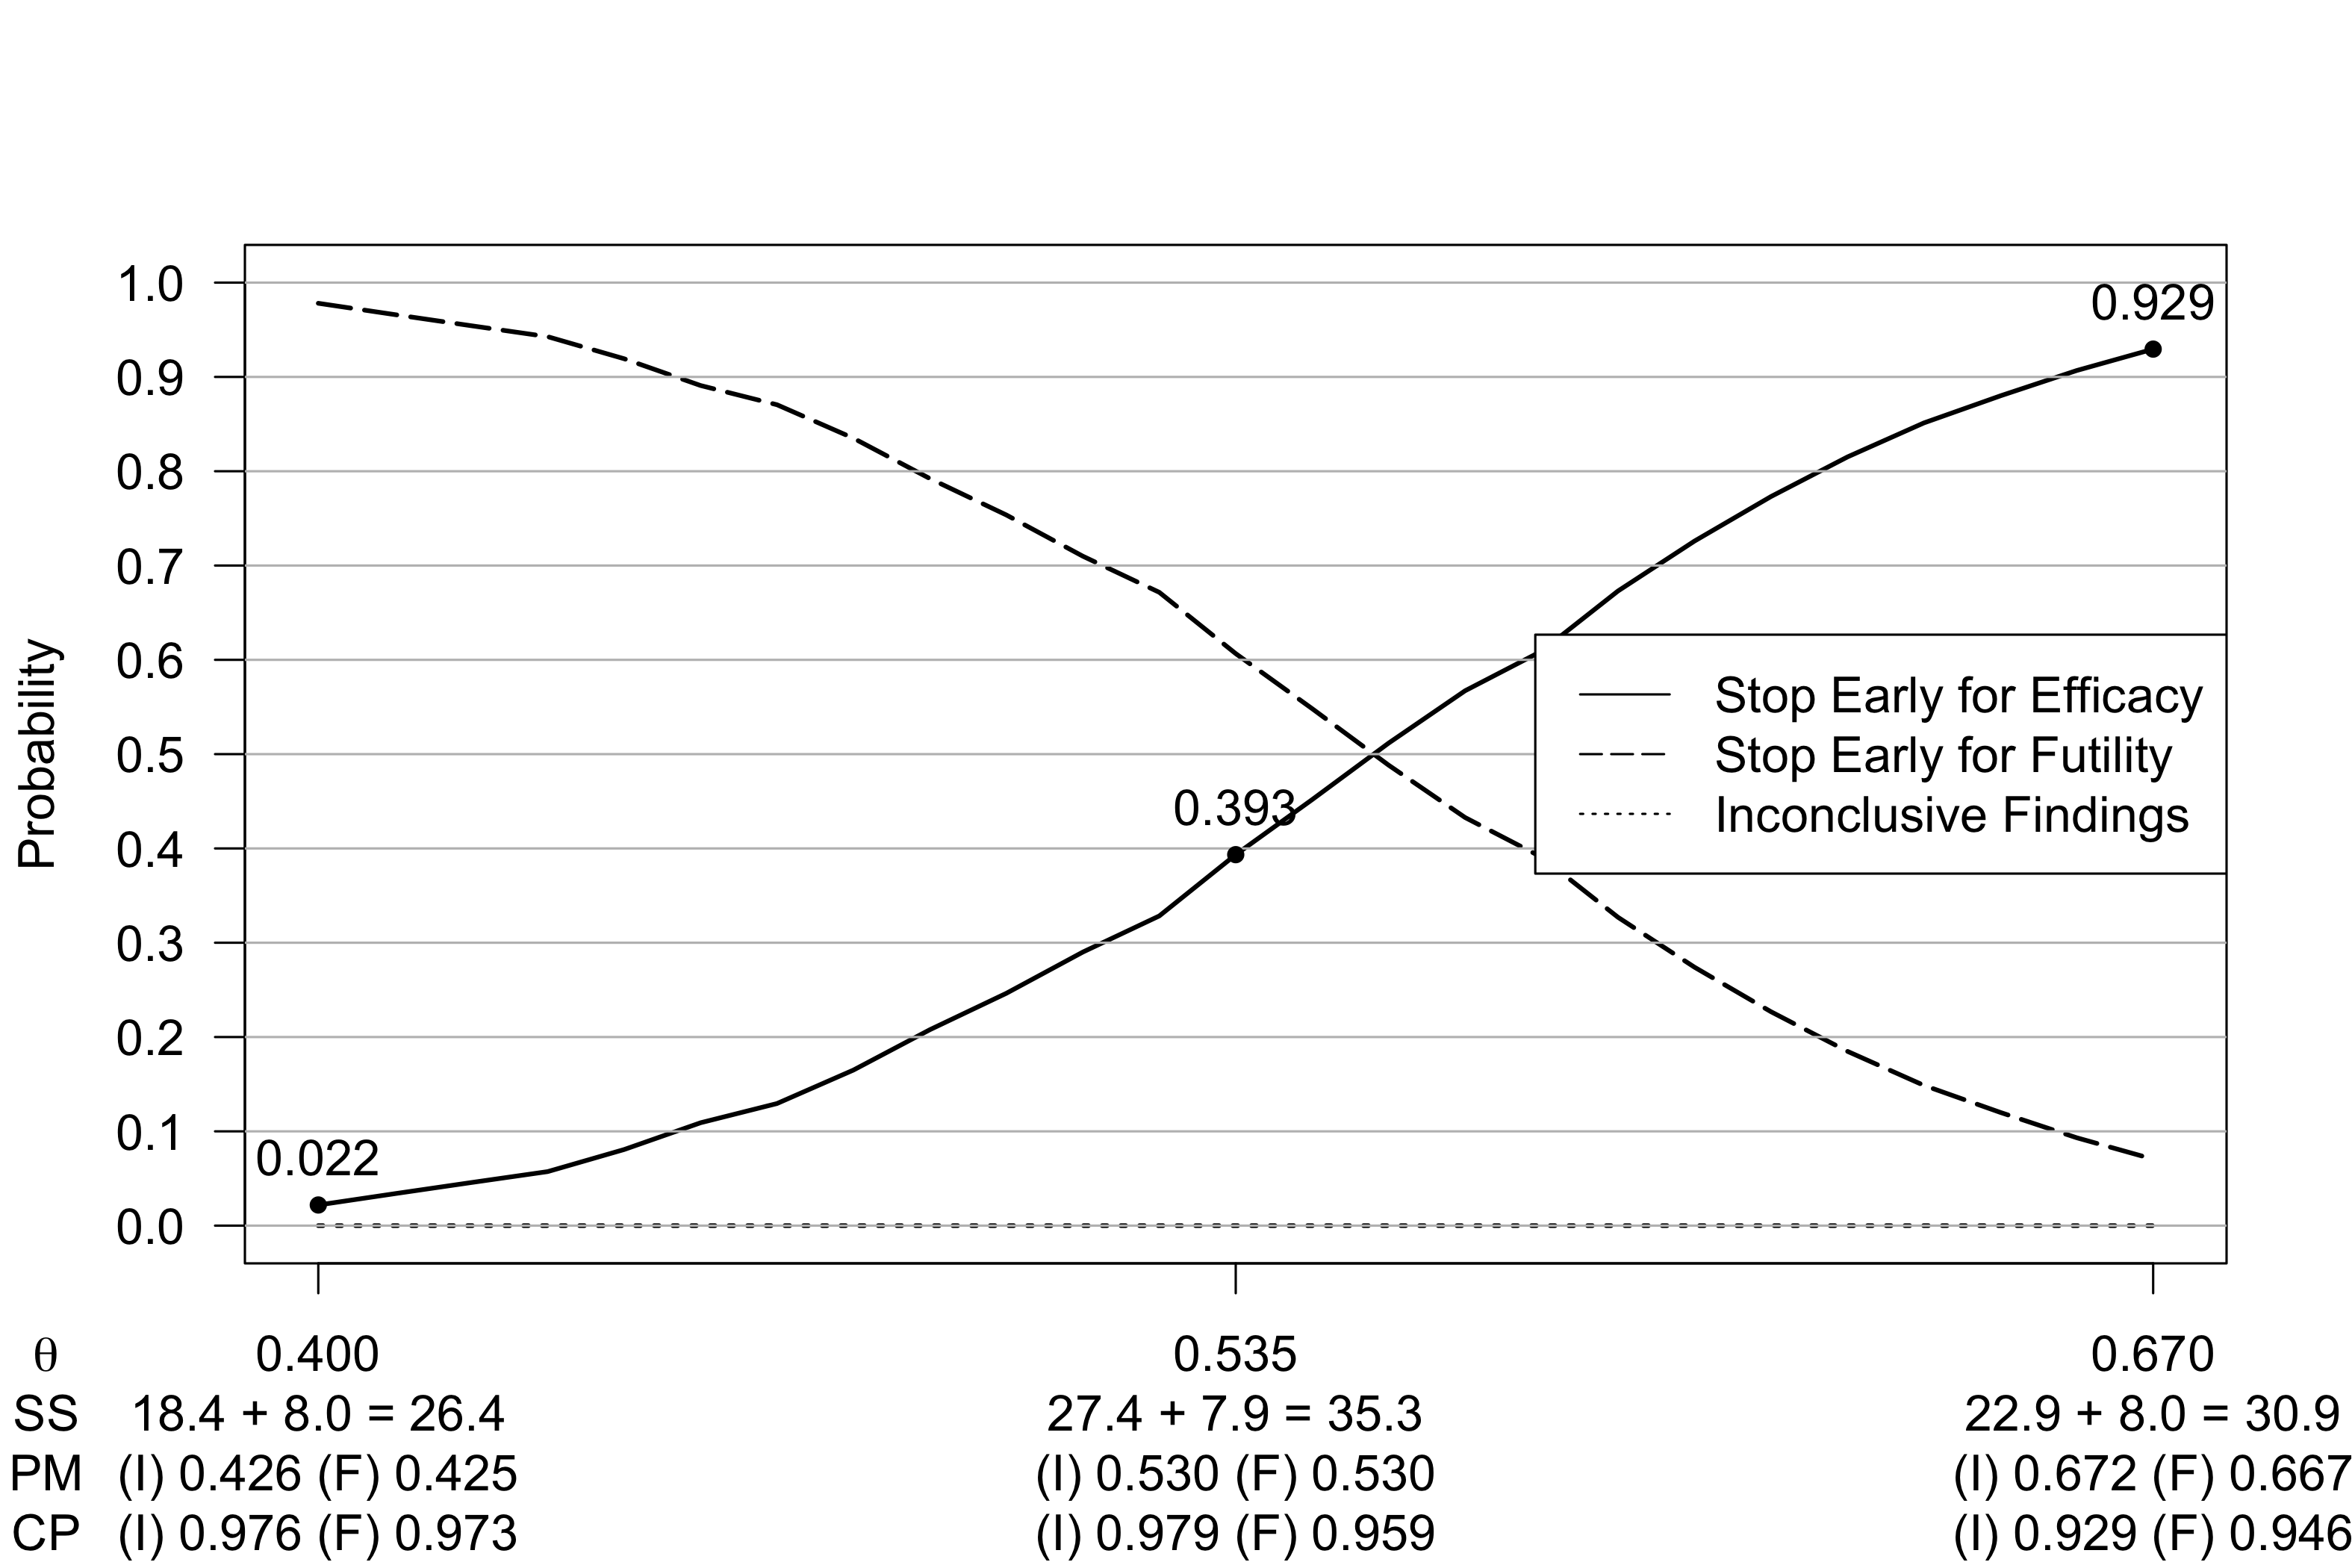
\includegraphics[width=7in]{./FIGURES/figureS2b.png}
 \caption{Modification of enthusiastic prior parameterization in Example \ref{sec:example1}. A, default enthusiastic prior (Figure \ref{fig:figure1}(c)). B, flattened enthusiastic prior (Figure \ref{fig:figure1}(d)). Both designs use concentrated skeptical prior (Figure \ref{fig:figure1}(b)).}
\label{fig:robustness1}
\end{center}\end{figure}

\begin{figure}\begin{center}

 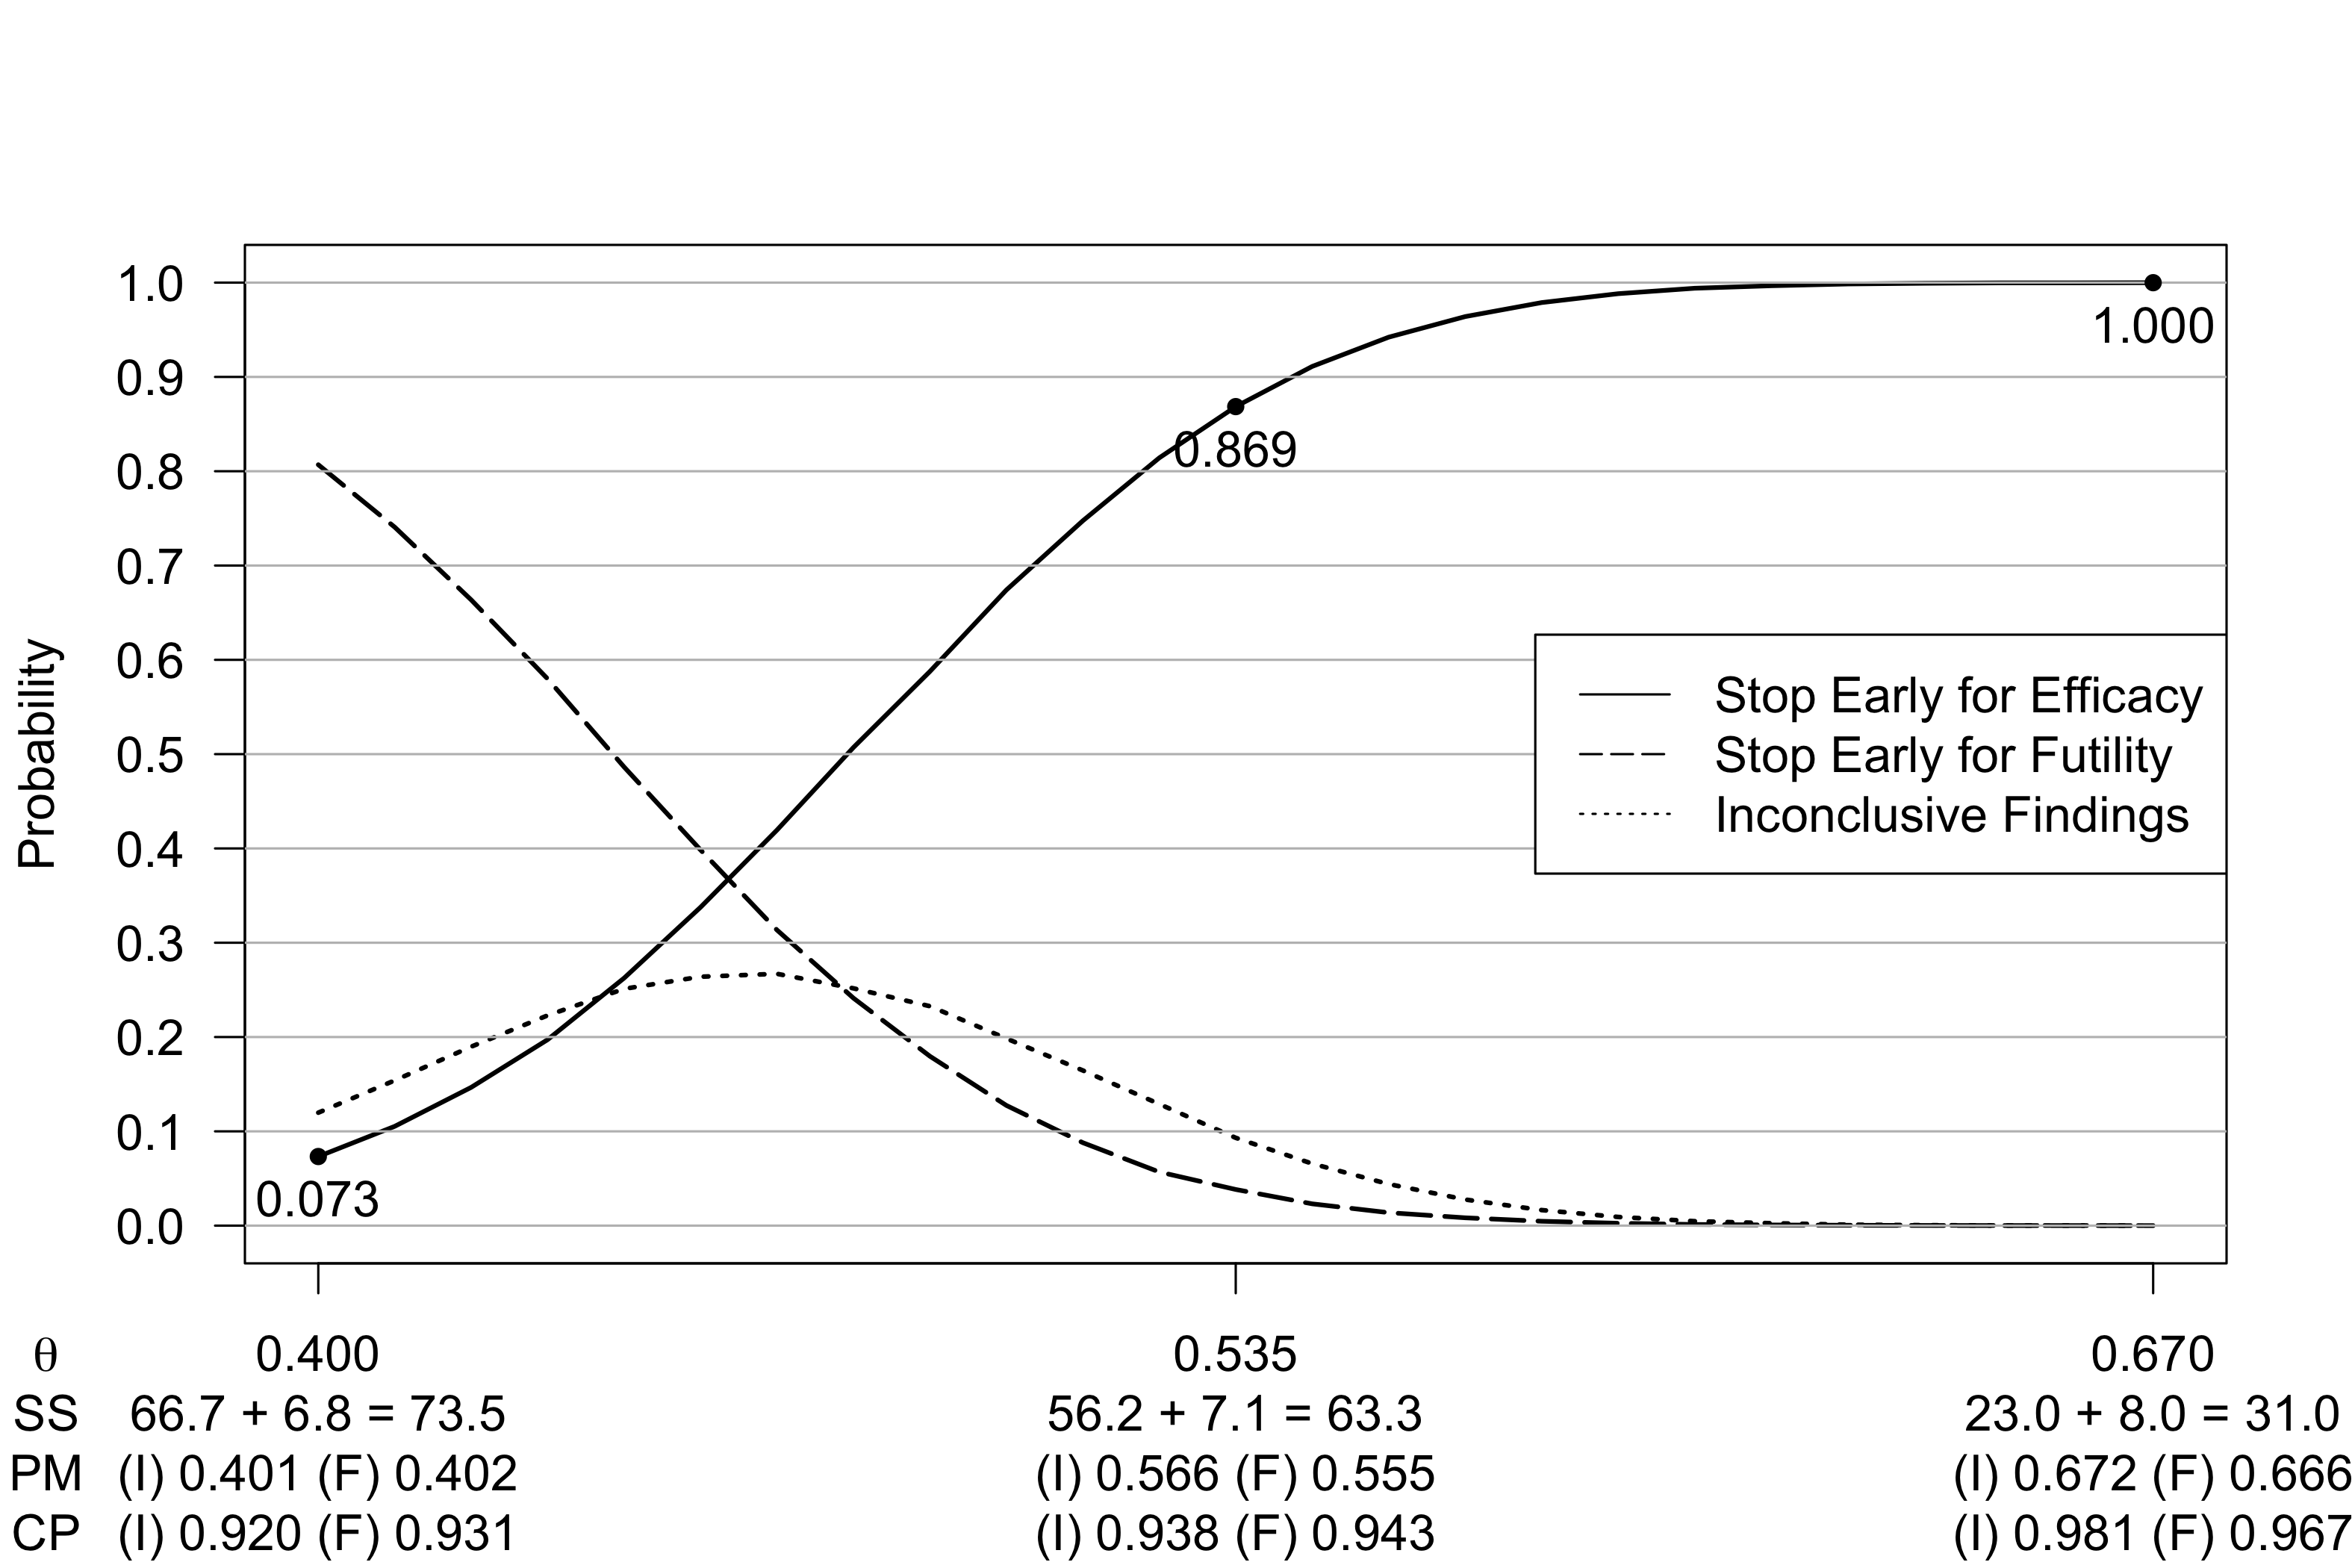
\includegraphics[width=7in]{./FIGURES/figureS2c.png}
 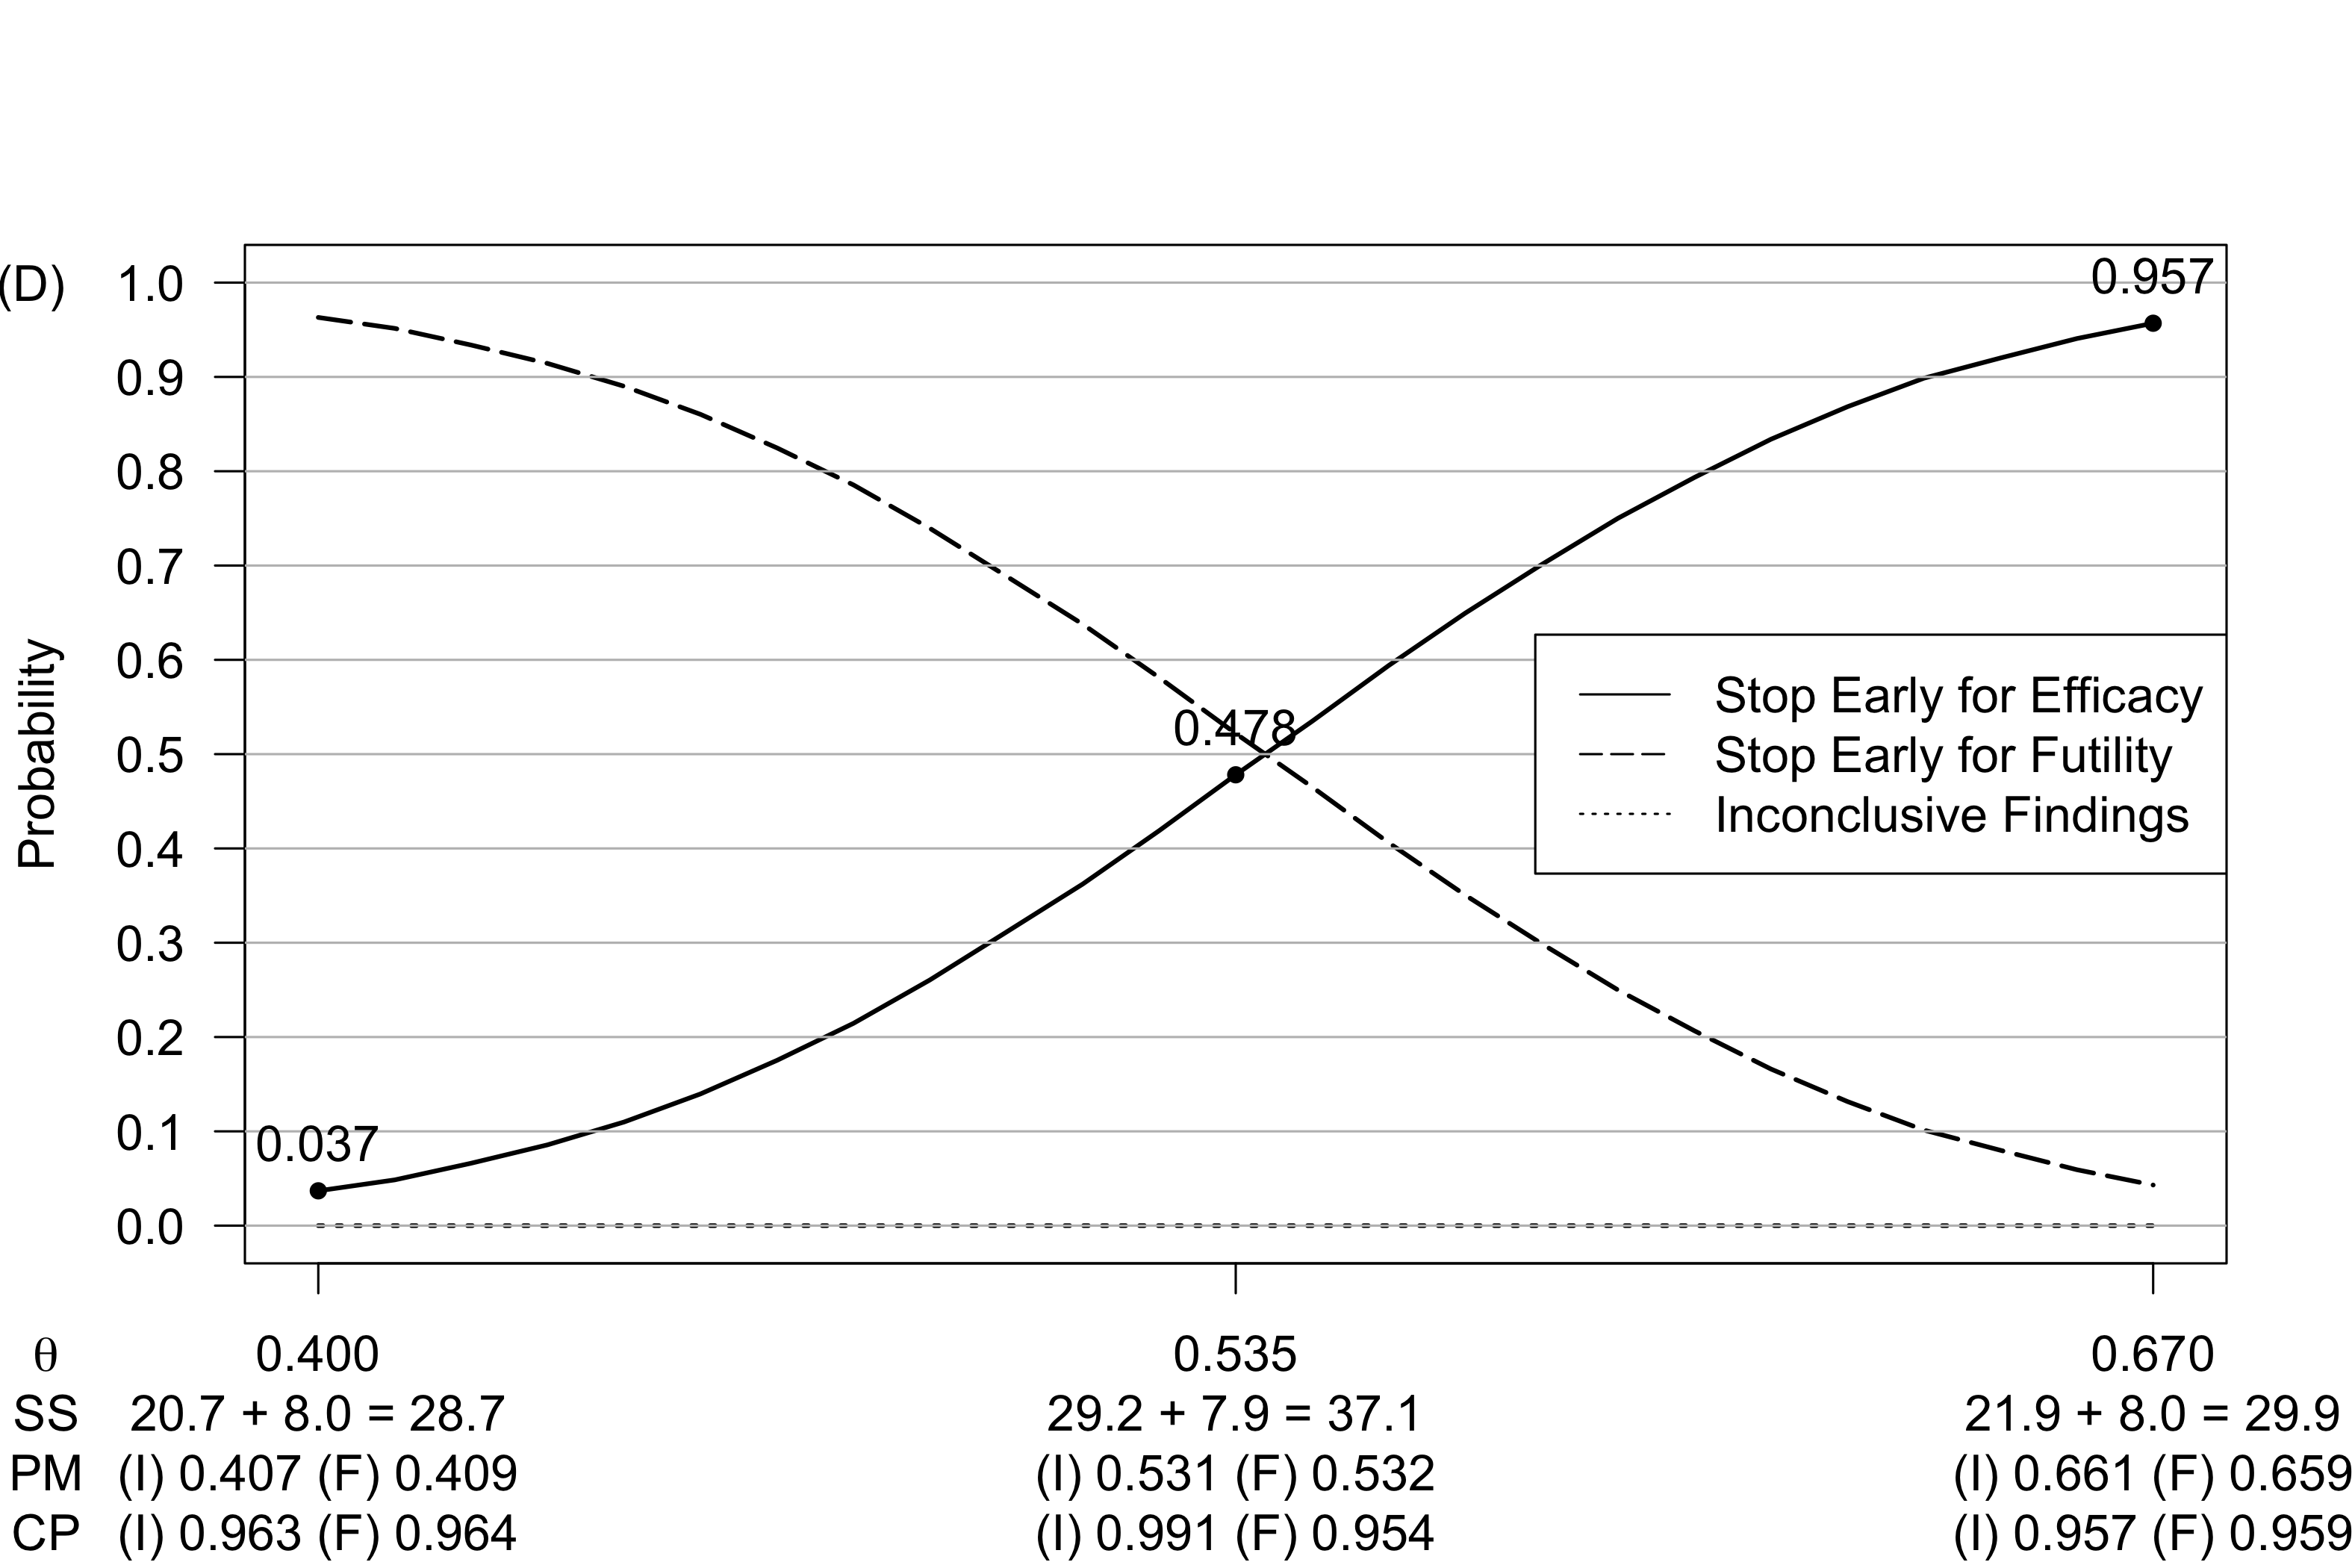
\includegraphics[width=7in]{./FIGURES/figureS2d.png}
 \caption{Modification of enthusiastic prior parameterization in Example \ref{sec:example1}. A, default enthusiastic prior (Figure \ref{fig:figure1}(c)). B, flattened enthusiastic prior (Figure \ref{fig:figure1}(d)). Both designs use default skeptical prior (Figure \ref{fig:figure1}(a)).}
\label{fig:robustness2}
\end{center}\end{figure}

%\section{BibTeX}
\newpage
\newpage
 \bibliographystyle{agsm}
 \bibliography{./References}	

\end{document}
